\documentclass{article}
\usepackage{iclr2027_conference,times}

\usepackage{amsmath,amssymb,amsthm,mathtools,bm}
\usepackage{booktabs,array,tabularx,multirow}
\usepackage{algorithm}
\usepackage[noend]{algpseudocode}
\usepackage{graphicx}
\usepackage{thmtools}
\usepackage{thm-restate}
\usepackage{xcolor}
\usepackage{colortbl}
\usepackage{microtype}
\usepackage{hyperref}
\usepackage[nameinlink,capitalise,noabbrev]{cleveref}
\usepackage{url}
\usepackage{wrapfig}
\usepackage{float}
\usepackage{enumitem}
\usepackage{titletoc}


% -----------------------------------------------------------------------------
% Theorem environments
% -----------------------------------------------------------------------------
\declaretheorem[numberwithin=section,name=Theorem]{theorem}
\declaretheorem[sibling=theorem,name=Proposition]{proposition}
\declaretheorem[sibling=theorem,name=Lemma]{lemma}
\declaretheorem[sibling=theorem,name=Corollary]{corollary}
\declaretheorem[sibling=theorem,name=Definition]{definition}
\declaretheorem[sibling=theorem,name=Assumption]{assumption}
\declaretheorem[sibling=theorem,name=Example]{example}
\declaretheorem[style=remark,sibling=theorem,name=Remark]{remark}

\crefname{theorem}{Theorem}{Theorems}
\Crefname{theorem}{Theorem}{Theorems}
\crefname{proposition}{Proposition}{Propositions}
\Crefname{proposition}{Proposition}{Propositions}
\crefname{lemma}{Lemma}{Lemmas}
\Crefname{lemma}{Lemma}{Lemmas}
\crefname{corollary}{Corollary}{Corollaries}
\Crefname{corollary}{Corollary}{Corollaries}
\crefname{definition}{Definition}{Definitions}
\Crefname{definition}{Definition}{Definitions}
\crefname{assumption}{Assumption}{Assumptions}
\Crefname{assumption}{Assumption}{Assumptions}
\crefname{equation}{Equation}{Equations}
\Crefname{equation}{Equation}{Equations}
\crefname{algorithm}{Algorithm}{Algorithms}
\Crefname{algorithm}{Algorithm}{Algorithms}
\crefname{table}{Table}{Tables}
\Crefname{table}{Table}{Tables}
\crefname{figure}{Figure}{Figures}
\Crefname{figure}{Figure}{Figures}
\crefname{section}{Section}{Sections}
\Crefname{section}{Section}{Sections}


% -----------------------------------------------------------------------------
% Notation
% -----------------------------------------------------------------------------
\newcommand{\R}{\mathbb{R}}
\newcommand{\E}{\mathbb{E}}
\newcommand{\Prob}{\mathbb{P}}
\newcommand{\KL}{\mathrm{KL}}
\newcommand{\TV}{\mathrm{TV}}
\newcommand{\1}{\mathbf{1}}
\newcommand{\norm}[1]{\left\lVert #1 \right\rVert_2}
\newcommand{\abs}[1]{\left\lvert #1 \right\rvert}
\newcommand{\pos}[1]{\left(#1\right)_{+}}
\newcommand{\Lset}{\mathcal{L}}
\newcommand{\Qclass}{\mathcal{Q}}
\newcommand{\Pclass}{\mathfrak{P}}
\newcommand{\Mclass}{\mathcal{M}}
\newcommand{\Xclass}{\mathfrak{X}}
\newcommand{\Rclass}{\mathfrak{R}}
\newcommand{\URisk}{\mathfrak{R}}
\newcommand{\PhiBar}{\overline\Phi}
\newcommand{\eps}{\varepsilon}
\newcommand{\mstar}{m^{\star}}
\newcommand{\mstarmax}{m^{\star\star}}
\newcommand{\argminop}{\operatorname*{arg\,min}}
\newcommand{\sgn}{\operatorname{sign}}
\newcommand{\Uset}{\mathcal{U}}
\DeclareMathOperator*{\argmin}{arg\,min}
\newcommand{\Mdown}{\mathcal{M}_{\downarrow}}
\DeclareMathOperator{\logit}{logit}
\title{CIS: Train–Inference-Mismatch-Aware RLVR via Calibrated Importance Sampling
% CIS: Calibrated Importance Sampling for\\
% Training--Inference Mismatch in LLM Reinforcement Learning}
% Training-Inference Mismatch Robust RLVR with Calibrated Importance Sampling
}
\author{Anonymous Authors}

% \iclrfinalcopy

\begin{document}
\maketitle

\begin{abstract}
We study training–inference mismatch in reinforcement learning with verifiable rewards (RLVR), where rollouts are sampled by an inference engine while gradients are computed by a training engine, assigning different probabilities to the same tokens. To account for this discrepancy in policy updates, we introduce CIS, a calibrated importance sampling method for mismatch correction. CIS is motivated by an empirically supported logit-displacement model that characterizes the mismatch as an additive displacement $\varepsilon_t$ in log-odds, with a confidence-invariant bulk distribution and a sparse residual component based on token confidence. This model motivates a confidence-aware truncation band that suppresses numerical noise on high-confidence tokens while preserving learning signals on less-confident tokens. Theoretically, we show that under the proposed mismatch model, CIS can provably reduce the explosive variance introduced by vanilla importance sampling. In comprehensive evaluation across five mathematical reasoning benchmarks, CIS achieves the highest average held-out accuracy among the evaluated token-level and sequence-level baselines, with low variability across seeds. Diagnostic analyses show that CIS acts on high-confidence tokens left untouched by the fixed-threshold baselines, while upward clipping of small importance weights reduces held-out accuracy despite increasing training reward. 
% Theoretically, under the proposed mismatch model, we bound the variance of CIS using the first exponential moment of the logit displacement, replacing the second-exponential-moment dependence of untruncated importance sampling while explicitly quantifying the bias introduced by truncation.
% We study the training-inference mismatch in reinforcement learning with verifiable reward (RLVR), where rollouts are sampled by an inference engine while gradients are computed by a training engine that assigns different probabilities to the same tokens. To mitigate this mismatch in the RLVR process, we introduce CIS, a calibrated importance sampling method for mismatch correction. The CIS is motivated by a careful-design logit-displacement model characterizing the mismatch as a displacement $\varepsilon_t$ in the log-odds that is independent of the model output. Based on this finding, CIS suppresses numerical noise and preserves the gradient signal by truncating the importance ratio with a confidence-aware band. Theoretically, CIS can provably reduce the explosive variance introduced by vanilla importance sampling. 
% CIS truncates the importance ratio with a confidence-dependent band, which suppresses numerical noise on high-confidence tokens while preserving the gradient signal on low-confidence ones, at the cost of a single elementwise operation. At the core of CIS is a logit-displacement model, which characterizes the mismatch as a displacement $\varepsilon_t$ in the log-odds that is independent of the token confidence, as supported by large-scale measurements. Under this model, we show that exact importance sampling incurs an explosive variance, and that the CIS band minimizes a bias--variance surrogate risk among all corrections that only shrink the ratio, with a provable reduction in variance. 
% Empirically, CIS achieves the highest held-out accuracy and the smallest variance across seeds among token-level and sequence-level baselines on 5 mathematical reasoning benchmarks. Diagnostic analyses show that CIS acts on high-confidence tokens that constant thresholds never reach, and that lifting the lower side of the band degrades held-out accuracy even as the training reward increases.
\end{abstract}
\section{Introduction}
\label{sec:introduction}

% Modern language-model RL is implemented by two software stacks. An inference engine such as vLLM or SGLang generates rollouts, while a training engine such as Megatron or FSDP recomputes log probabilities and backpropagates gradients. Different kernels, parallelism layouts, reduction orders, precisions, and decode paths make these stacks numerically distinct even when they load the same parameters \citep{yao2025tis,he2025nondeterminism,qi2025fp16}. The discrepancy is especially consequential in mixture-of-experts models. A small numerical perturbation can change a discrete top-$k$ routing decision, so the training path may traverse experts that did not generate the sampled token \citep{ling2025ring,ma2025r3}. The mismatch can then affect both the token probability and the conditional mean of the gradient payload.

% Practice has produced two different repairs. Truncated importance sampling (TIS) caps the engine ratio \citep{ionides2008truncated,yao2025tis}; IcePop zeroes every ratio outside a fixed interval \citep{ling2025ring}. Both require choices outside the underlying RL objective. This leaves three questions unanswered: why should a large ratio be capped rather than removed, when should it instead be removed, and what uncertainty assumptions make either operation uniformly valid?

% \paragraph{Our view.}
% An uncertainty class is not merely a regularizer around a fixed algorithm. Together with a decision criterion, it selects the token-level operator and determines the boundary of its guarantee. A bounded-ratio class treats every payload as valid but potentially influential, leading to a projection onto an influence budget. A localized corrupted channel allows a small fraction of payload means to be unknown without imposing a zero-mean condition, leading to a clean-fidelity versus corrupted-exposure tradeoff. The cap and the gate are therefore solutions to different statistical problems rather than interchangeable heuristics.

% Our contributions are threefold.
% \begin{itemize}
%     \item We formalize geometry--operator correspondence through two requirements: an operator must minimize a bias constant uniformly over a stated observation-law class, and a matching hard instance must characterize the boundary beyond which its guarantee fails. This follows the closed-form-plus-lower-bound proof organization of \citet{shi2023distributionally}, while changing the statistical object from a robust Bellman functional to a ratio-weighted gradient estimator.
%     \item We prove a complete density-band correspondence. A cap covering the band is exactly unbiased; under a fixed influence budget it is the unique pointwise projection for every admissible ratio law; and an essential escape component places the observation law outside every finite band and creates a bias floor of at least $\eps B e^{\sigma}$ for every band-faithful cap.
%     \item We prove a complete localized-corruption correspondence. Without localization, the cap-versus-gate choice is not identifiable from the class. With localization, the uniform-risk optimal rule is the identity outside the escape set and $\min\{k,m^{\star}\}$ inside it. Hard zeroing is optimal if and only if positive clean escape mass is at most $\eps/(1-\eps)$, and an attaining-member construction matches the uniform constant for every measurable operator.
% \end{itemize}

\paragraph{Notation.}
We use plain letters such as $x$ to denote scalars, lowercase bold letters such as
$\mathbf{x}$ to denote vectors, and calligraphic letters such as $\mathcal{F}$ to
denote sets and function classes. For a vector $\mathbf{x}$, $\|\mathbf{x}\|_2$
denotes its $\ell_2$-norm. For a scalar $x \in (0,1)$, $\logit x := \log\frac{x}{1-x}$.
\section{Preliminaries}
\label{sec:prelim}

\subsection{Training--inference mismatch}
\label{sec:prelim_mismatch}

In current RL post-training frameworks, rollouts are generated by an inference
engine (vLLM, SGLang) while gradients are computed by a training engine (FSDP,
Megatron). The two load the same parameters $\theta$, yet differing kernel
implementations, reduction orders, and numerical precisions make them assign
different probabilities to the same token,
$\pi_{\mathrm{train}}(y_t\mid x,y_{<t};\theta)\ne
\pi_{\mathrm{infer}}(y_t\mid x,y_{<t};\theta)$,
so that rollouts that are nominally on-policy are in fact off-policy with
respect to the training-engine policy. The problem is more severe on
mixture-of-experts models, where routing is a discrete top-$k$ decision and a
small numerical perturbation can change which experts are activated.

\subsection{Training--inference mismatch in RLVR}
\label{sec:prelim_rlvr}

Rollouts are sampled from the inference engine while gradients are computed
under the training-engine policy. For the token-level GRPO surrogate evaluated
on the observed rollout prefixes, correcting the conditional distribution of
each sampled token introduces the importance ratio
\begin{equation}
\mathcal J(\theta)
=
\E_{x\sim\mathcal D,\;\{y_i\}_{i=1}^{G}\sim\pi_{\mathrm{infer}}(\cdot\mid x;\theta_{\mathrm{old}})}
\left[
\frac{1}{G}\sum_{i=1}^{G}\frac{1}{\abs{y_i}}\sum_{t=1}^{\abs{y_i}}
k_{i,t}\,
\min\Big(
\rho_{i,t}\hat A_{i,t},\;
\operatorname{clip}\big(\rho_{i,t}\big)\hat A_{i,t}
\Big)
\right],
\label{eq:objective}
\end{equation}
where
$\rho_{i,t}=\pi_{\mathrm{train}}(y_{i,t}\mid x,y_{i,<t};\theta)\big/
\pi_{\mathrm{train}}(y_{i,t}\mid x,y_{i,<t};\theta_{\mathrm{old}})$
and
$k_{i,t}=\pi_{\mathrm{train}}(y_{i,t}\mid x,y_{i,<t};\theta_{\mathrm{old}})\big/
\pi_{\mathrm{infer}}(y_{i,t}\mid x,y_{i,<t};\theta_{\mathrm{old}})$,
with $\theta_{\mathrm{old}}$ the parameter snapshot at rollout time and
$\hat A_{i,t}$ the group-normalized advantage.
Here $k_{i,t}$ corrects the next-token distribution conditional on the observed
prefix $(x,y_{i,<t})$; it does not importance-weight the distribution of the
prefix itself. The update ratio $\rho_{i,t}$ is handled by the clip of standard
PPO; the mismatch ratio $k_{i,t}$ carries the discrepancy of
Section~\ref{sec:prelim_mismatch} and is the subject of the rest of this paper.
% \section{The CIS Framework}
% \label{sec:cis}

% \subsection{A two-channel model of the mismatch}
% \label{sec:two_channel}

% \begin{wrapfigure}{r}{0.5\textwidth}
% \vspace{-1.2\baselineskip}
% \centering
% 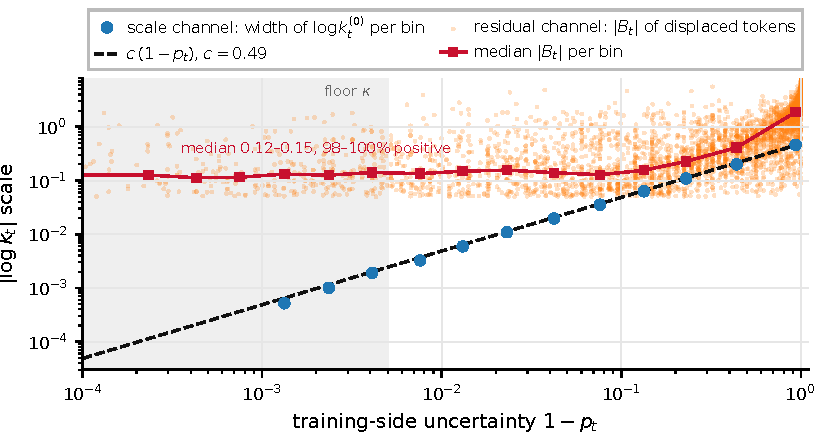
\includegraphics[width=0.5\textwidth]{figures/two_channel.pdf}
% \vspace{-0.6\baselineskip}
% \caption{The two channels on the same tokens (trained MoE policy, 509k tokens). Blue: $|\log k_t|$ when both engines score the same snapshot, and its width per uncertainty bin, which follows $c\,(1-p_t)$ with $c=0.49$ over three decades. Orange: the residual displacement $|B_t|$ on the same tokens, for tokens displaced by more than ten times the storage resolution, and its per-bin median; it stays at $0.12$ to $0.15$ across $1-p_t\in[3\times10^{-4},0.15]$ and is positive on $98$ to $100\%$ of these tokens. The channels overlap only at $1-p_t\gtrsim0.3$; the shaded band is the floor $\kappa$ of \Cref{sec:algorithm}. Details in \Cref{sec:exp_measurement}.}
% \label{fig:two_channel}
% \vspace{-0.8\baselineskip}
% \end{wrapfigure}

% We measured $k_{i,t}$ systematically on large-scale rollouts; experimental
% details are given in \Cref{sec:exp_measurement}. Write
% $p_{i,t}=\pi_{\mathrm{train}}(y_{i,t}\mid x,y_{i,<t};\theta_{\mathrm{old}})$
% for the training-side probability of the token that was actually sampled, and
% drop the index $i$ in what follows. Two facts emerge
% (\Cref{fig:two_channel}). First, the conditional law of $\log k_t$ forms a
% \emph{scale family}, $\log k_t \,\big|\, p_t \overset{d}{=} c\,(1-p_t)\,Z$ with
% the law of $Z$ not depending on $p_t$, so that the shape is fixed and the width
% is proportional to $1-p_t$, where $c>0$ is a constant of the model and engine
% configuration. Second, a small fraction of tokens does not obey this law: their
% deviations do not scale with $1-p_t$, and their magnitude is set by router
% logit gaps and by the storage resolution of the log-probabilities. These two
% facts give the following model.

% \begin{definition}[Two-channel model]
% \label{def:two_channel}
% Conditionally on $p_t$, the observed log-ratio is generated as
% \begin{equation}
% \log k_t
% \;=\;
% c\,(1-p_t)\,Z_t
% \;+\;
% B_t ,
% \label{eq:two_channel}
% \end{equation}
% where the scale component satisfies $Z_t\sim F_Z$ with $F_Z$ independent of
% $p_t$, $\E[Z_t]=0$, $\E|Z_t|<\infty$, $\E[(Z_t)_{+}]>0$, and an upper tail
% that is generalized Pareto with shape $\xi_+\in(0,1)$, no parametric form
% being assumed for $F_Z$; and the residual component satisfies
% $\Prob(B_t\ne0)\le\eps$ and $-B_{\min}\le B_t\le B_{\max}$ with
% $B_{\min},B_{\max}$ independent of $p_t$ on the high-confidence range
% $1-p_t\le\varphi_0$, the event $\{B_t\ne0\}$ being
% independent of $(Z_t,p_t)$ while the value of $B_t$ within the envelope is
% left unmodeled.
% \end{definition}

% \subsection{Estimand and robust risk}
% \label{sec:robust_risk}

% The change of measure $\E[k\,\ell']=\E_{y\sim\pi_{\mathrm{train}}}[\ell']$
% holds exactly; the question is not whether it is valid but which functional of
% the configuration we optimize. The two channels of \Cref{def:two_channel}
% differ on precisely this point. The scale channel is determined by $(c,F_Z)$:
% given a model and an engine configuration it is the same law on every batch.
% The residual channel is determined by which tokens happen to fall on a routing
% boundary or below the storage resolution, and is stable neither across batches
% nor across configurations; carrying it in the target would make the estimand
% move from batch to batch, and no threshold compiled from it would transfer. We
% therefore take the gradient induced by the scale channel alone,
% \begin{equation}
% G_0:=\E\big[e^{\,c(1-p_t)Z_t}\,\ell'\big],
% \label{eq:estimand}
% \end{equation}
% as the estimand; it coincides with $\E[k\,\ell']$ at $\eps=0$, and the residual
% becomes a nuisance---absent from the target, present in every sample.

% For a given sampling law $P$ the mean-squared error of the estimator is
% $\mathcal E_0(\Mclass;P)=\E_P\norm{\widehat G_{\Mclass}-G_0}^{2}$. It cannot be
% optimized directly: $B_t$ is characterized only at the level of sets and
% carries no law to integrate against. We therefore optimize
% \begin{equation}
% \mathcal E(\Mclass)
% :=
% \sup_{P\in\Uset}
% \left\{
% \Big(\sum_p\norm{b_p(\Mclass)}\Big)^{2}
% +\frac{1}{n}\E_P\big[\Mclass^{2}\norm{\ell'}^{2}\big]
% \right\},
% \label{eq:robust_risk}
% \end{equation}
% where
% $b_p(\Mclass)=\E\big[\big(\Mclass(k_t)-e^{\,c(1-p_t)Z_t}\big)\ell'_t\mid p_t=p\big]\,
% \Prob(p_t=p)$
% is the contribution of confidence level $p$ to the bias, and
% $\Uset=\big\{P:\ \log k_t=c(1-p_t)Z_t+B_t,\ Z_t\sim F_Z,\
% \Prob(B_t\ne0)\le\eps,\ -B_{\min}\le B_t\le B_{\max}\big\}$.

% \begin{theorem}[CIS operator, informal]
% \label{thm:cis_informal}
% Under \Cref{def:two_channel}, and when the displacement of the residual channel
% in standardized coordinates is sufficiently large, the minimizer of the robust
% risk over the shrinkage class is
% \begin{equation}
% \log\Mclass^{\star}(k_t,p_t)
% =
% \argminop_{\Mclass\in\Mdown}\mathcal E(\Mclass)
% =
% \min\Big(\log k_t,\;\lambda\,(1-p_t)\Big),
% \label{eq:cis_operator}
% \end{equation}
% where the slope is $\lambda=c\,\tau^{\star}$ and the threshold $\tau^{\star}$
% is uniquely determined by $F_Z$, the residual occurrence rate $\eps$, and the
% sample size $n$.
% \end{theorem}

% \subsection{The deployed algorithm}
% \label{sec:algorithm}

% \Cref{thm:cis_informal} gives a one-sided bound whose width scales with
% $1-p_t$. One correction is needed at the edge of the model's identifiable
% range: as $p_t\to1$ the observed width of $\log k_t$ saturates at the storage
% resolution of the log-probabilities rather than following $c(1-p_t)$, so an
% unfloored band would truncate quantization noise rather than mismatch. We
% therefore floor the scale variable at $\kappa$, which gives \Cref{alg:cis}. The
% two hyperparameters admit measured defaults rather than a search:
% \Cref{thm:cis_informal} compiles $\lambda=c\,\tau^{\star}$, and $\kappa$ is the
% storage resolution of the log-probabilities.

% \begin{wrapfigure}{r}{0.5\textwidth}
% \vspace{-\baselineskip}
% \begin{minipage}{0.5\textwidth}
% \begin{algorithm}[H]
% \caption{Calibrated importance sampling (CIS)}
% \label{alg:cis}
% \begin{algorithmic}[1]
% \Require $\ell^{\mathrm{train}}_j$, $\ell^{\mathrm{infer}}_j$, $\ell'_j$ for
% the $n$ tokens of the batch; $\lambda$; $\kappa$
% \For{$j=1,\dots,n$}
%   \State $\log k_j\gets\ell^{\mathrm{train}}_j-\ell^{\mathrm{infer}}_j$,\quad
%   $p_j\gets\exp(\ell^{\mathrm{train}}_j)$
%   \State $w_j\gets\exp\big(\min\{\log k_j,\;
%   \lambda\max(1-p_j,\kappa)\}\big)$
% \EndFor
% \State \Return $\widehat G_{\mathrm{CIS}}
% =\frac{1}{n}\sum_{j=1}^{n}\operatorname{stopgrad}(w_j)\,\ell'_j$
% \end{algorithmic}
% \end{algorithm}
% \end{minipage}
% \end{wrapfigure}

% The operator adds one elementwise pass and no forward or backward computation.
% Three implementation details are load-bearing: the inference-side
% log-probability must be the raw value recorded at the sampling step, with no
% temperature rescaling or renormalization applied afterwards; the weight must be
% detached, since $k_t$ is data rather than a function of $\theta$; and the floor
% must be applied to $1-p_t$ before multiplication by $\lambda$, not to the
% resulting band.
\section{The CIS Framework}
\label{sec:cis}
\subsection{A logit-displacement model of the mismatch}
\label{sec:logit_model}

\begin{wrapfigure}{r}{0.45\textwidth}
\vspace{-1.2\baselineskip}
\centering
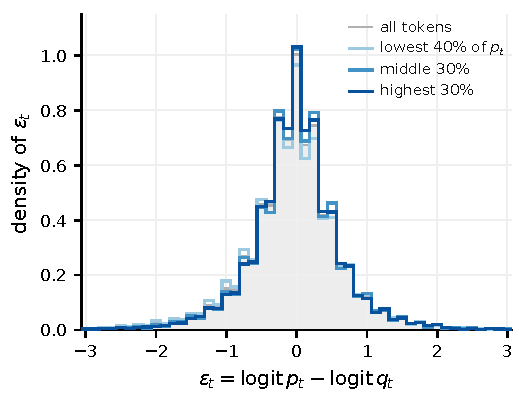
\includegraphics[width=0.45\textwidth]{figures/fig_eps_dist.pdf}
\vspace{-1.4\baselineskip}
\caption{Distribution of $\varepsilon_t$ on a trained MoE, pooled and split by
confidence $p_t$ (histogram bin width $0.125$). The conditional laws coincide.}
\label{fig:eps_dist}
\vspace{-0.8\baselineskip}
\end{wrapfigure}

We measured the pair $(p_t,q_t)$ systematically on large-scale rollouts;
experimental details are given in \Cref{sec:exp_measurement}. Write $p_t=\pi_{\mathrm{train}}(y_t\mid x,y_{<t};\theta_{\mathrm{old}}),
\qquad
q_t=\pi_{\mathrm{infer}}(y_t\mid x,y_{<t};\theta_{\mathrm{old}})$
for the two engines' probabilities of the token that was actually sampled, and
drop the trajectory index $i$ in what follows. The measurements show that the
discrepancy between the two engines is stationary in the log-odds coordinate,
which gives the following model.

\begin{definition}[Logit-displacement model]
\label{def:logit_displacement}
Conditionally on the prefix $h_t$, the two engines' probabilities of the sampled
token satisfy
\begin{equation}
\logit q_t
\;=\;
\logit p_t-\varepsilon_t ,
\qquad
\varepsilon_t\perp p_t ,
\label{eq:logit_displacement}
\end{equation}
where $\mu:=\E[e^{\varepsilon_t}]$ and $\exists\,\alpha>1:\ \E[e^{\alpha\varepsilon_t}]<\infty$.
\end{definition}

Here $\varepsilon_t$ is the log-odds displacement of the inference engine
relative to the training engine on that token, and the substance of the model is
that its distribution does not depend on the confidence.
\Cref{fig:eps_dist} shows the distribution of $\varepsilon_t$, pooled and split
into three confidence groups; a detailed empirical analysis is given in
\Cref{sec:experiments}.

% Solving \eqref{eq:logit_displacement} for the mismatch ratio gives
% \begin{equation}
% k_t
% \;=\;
% p_t+(1-p_t)\,e^{\varepsilon_t}.
% \label{eq:k_geometry}
% \end{equation}
\subsection{Why a correction is needed}
\label{sec:why_correction}

A gradient update uses $n$ tokens (all tokens of all trajectories in the batch).
Write the payload of the $j$-th token as
$\ell'_j=\nabla_\theta\min\big(\rho_j\hat A_j,\operatorname{clip}(\rho_j)\hat A_j\big)$,
the gradient of the surrogate term in \eqref{eq:objective}. Since $k_j$ does not
depend on $\theta$, the gradient of the objective and its $n$-sample estimator
are $G_0:=\nabla_\theta\mathcal J=\E[k\,\ell']$ and
$\widehat G:=\frac{1}{n}\sum_{j=1}^{n}k_j\,\ell'_j$, and we measure the quality
of the estimate by the mean-squared error
$\E\big\|\widehat G-G_0\big\|_2^2$.

\begin{theorem}[Informal]
\label{thm:exact_risk}
Let $k_t$ satisfy \Cref{def:logit_displacement}. Then
\begin{equation}
\E\big\|\widehat G-G_0\big\|_2^2
\;=\;
\frac{1}{n}\Big(c_1+c_2\,\E\big[e^{2\varepsilon_t}\big]\Big),
\label{eq:exact_risk}
\end{equation}
where $c_1,c_2>0$ depend only on the joint law of $(p_t,\ell'_t)$ and not on
$\varepsilon_t$.
\end{theorem}
\begin{wrapfigure}{r}{0.42\textwidth}
\vspace{-1.0\baselineskip}
\centering
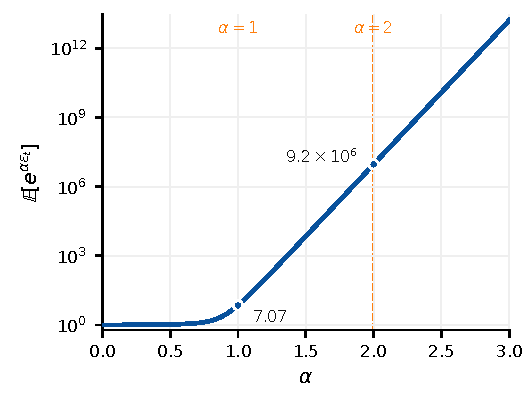
\includegraphics[width=0.42\textwidth]{figures/fig_mgf.pdf}
\vspace{-1.4\baselineskip}
\caption{$\E[e^{\alpha\varepsilon_t}]$ computed from the measured
$\varepsilon_t$.}
\label{fig:mgf}
\vspace{-0.8\baselineskip}
\end{wrapfigure}

\Cref{fig:mgf} shows $\E[e^{\alpha\varepsilon_t}]$ computed from the measured
displacements; details are given in \Cref{app:mgf}. At $\alpha=2$ we obtain
$\E[e^{2\varepsilon_t}]=9.2\times10^{6}$. Our training configuration uses
$n\approx4\times10^{3}$ tokens per update, so the variance term in
\eqref{eq:exact_risk} is of order $10^{3}$.

% One of the reason of this explosive variance is contributed by the explosion of the importance sampling factor $k_j$ when the inference engine and the training engine disagree signficiantly. 
% To mitigate this explosive variance, many existing works introduce some bias in exchane for an well-conditioned variance especially by downweighting the suspicious (overly large) importance sampling factor $k_j$ with the knowledge of it's likelihood $p_j$. Systematically, we can formulate their estimator as ... $\hat G$..

% $\mathcal M -> f(k_j, p_j)$,

% $\hat G_f = 1 / n \sum_{j=1}^n  f(k_j, p_j) \ell_j'$ where $f(k_j, p_j) \in \mathcal F: \{f: 0 \le f(k, p) \le k \}$
% $\hat G_f = 1 / n \sum_{j=1}^n  f(k_j, p_j), where $f(k, j)$ is the corrected importance sampling factor with the liklihood $p_j$ satisfying $f(k, p) \in [0, k]$ implying that $f(k, p)$ cannot exceed the original importance sampling factor. 

We must therefore act on $k_t$. Our objective remains the minimization of
$\E\big\|\widehat G-G_0\big\|_2^2$, and by \Cref{thm:exact_risk} the exact
correction has already driven the bias to zero and placed the entire risk in the
variance; any improvement must come from the opposite direction, by introducing
some bias in exchange for a smaller variance so that their sum is reduced.
Existing token-level corrections do exactly this: TIS caps $k_t$
\citep{cite}, IcePop masks tokens falling outside an interval \citep{cite}, and
KPop masks by a KL threshold \citep{cite}, all of which attenuate a weight but
never amplify it. We write such corrections uniformly as an operator
$\Mclass:(0,\infty)\times(0,1)\to(0,\infty)$ acting on the mismatch ratio, with
estimator


% we note $G_{\mathcal M}$ = \EE M(k_j, p_j) \ell_j'$ where the expectation comes from the randomness of the dataset. 

%\EE [M(k_j, p_j)^2 \cdot \|\ell'\|]
\begin{equation}
\widehat G_{\Mclass}
:=\frac{1}{n}\sum_{j=1}^{n}\Mclass(k_j,p_j)\,\ell'_j ,
\qquad
\Mclass\in\Mdown
:=\big\{\Mclass:\ 0<\Mclass(k,p)\le k\ \ \forall\,(k,p)\big\}.
\label{eq:operator_class}
\end{equation}
The restriction to $\Mdown$ agrees with the methods above and has a reason of
its own: by \eqref{eq:k_geometry} the ratio satisfies $k_t\ge p_t$, so its lower
side is bounded by construction and the variance comes entirely from the upper
side, while amplifying a weight would increase the bias and the variance at
once.
\subsection{The optimal operator}
\label{sec:optimal_operator}

For independent token contributions the mean-squared error of
$\widehat G_{\Mclass}$ admits the upper bound
\begin{equation}
\E\big\|\widehat G_{\Mclass}-G_0\big\|_2^2
\;\le\;
\big\|\E[\Mclass\,\ell']-G_0\big\|_2^2
+\frac{1}{n}\,\E\big[\Mclass^2\|\ell'\|_2^2\big]
\;=:\;
\mathcal R(\Mclass),
\label{eq:surrogate_risk}
\end{equation}
and we take $\mathcal R$ as the surrogate risk and minimize it over the
shrinkage class.

\begin{theorem}[CIS operator, informal]
\label{thm:cis_informal}
Under \Cref{def:logit_displacement},
\begin{equation}
\Mclass^{\star}(k_t,p_t)
=
\argminop_{\Mclass\in\Mdown}\mathcal R(\Mclass)
=
\min\big\{k_t,\;1+\lambda\,(1-p_t)\big\},
\label{eq:cis_operator}
\end{equation}
% absolute constant depends on the momentum of $\varepsilon$, sample size $n$ and the distribution of 
% $\ell'_t$ under distribution $p_t$.
% distribution of $\ell_t$ under $p_t$. 

% $M(x, y) = \alpha x + (1 - \alpha) (1 + \lambda (1 - y))$
% x \le (1 + \lambda (1 - y))
where $\lambda>0$ is uniquely determined by the law of $e^{\varepsilon_t}$, the
sample size $n$, and the joint law of $(p_t,\ell'_t)$.
\end{theorem}

\begin{remark}
\Cref{thm:cis_informal} is an upper bound that tightens with confidence: the
more certain the model is on a token, the closer to one the admissible weight;
the less certain it is, the larger the deviation admitted. On high-confidence
tokens the two engines' probability ratio should already be close to one, so a
large deviation there is more likely to come from numerical noise than from a
genuine difference between the two distributions; on low-confidence tokens the
ratio is dispersed to begin with, and clipping it too tightly discards useful
gradient signal.
\end{remark}

\begin{theorem}[Informal]
\label{thm:cis_risk}
Under the operator of \Cref{thm:cis_informal},
\begin{equation}
\E\big\|\widehat G_{\Mclass^{\star}}-G_0\big\|_2^2
\;\le\;
c_3\,\E\big[(e^{\varepsilon_t}-1-\lambda)_+\big]^2
+\frac{1}{n}\Big(c_1'+c_2\,\E\big[\min(e^{\varepsilon_t},1+\lambda)^2\big]\Big),
\label{eq:cis_risk}
\end{equation}
where $c_2$ is the same constant as in \Cref{thm:exact_risk}, and
$c_1',c_3>0$ likewise depend only on the joint law of $(p_t,\ell'_t)$.
\end{theorem}

\begin{remark}
Compared with \Cref{thm:exact_risk}, the term $\E[e^{2\varepsilon_t}]$ in the
variance is replaced by $\E[\min(e^{\varepsilon_t},1+\lambda)^2]$, which
satisfies
$\E[\min(e^{\varepsilon_t},1+\lambda)^2]\le(1+\lambda)\,\E[e^{\varepsilon_t}]
=(1+\lambda)\,\mu$: the exponent drops from two to one, and the second
exponential moment is traded for the first, which is the constant $\mu$ of
\Cref{def:logit_displacement}, read off \Cref{fig:mgf} at $\alpha=1$ and both
finite and estimable. The price is the bias term, set by the exceedance that the
operator removes and decreasing in $\lambda$.
\end{remark}

\begin{wrapfigure}{r}{0.5\textwidth}
\vspace{-\baselineskip}
\begin{minipage}{0.5\textwidth}
\begin{algorithm}[H]
\caption{Calibrated importance sampling (CIS)}
\label{alg:cis}
\begin{algorithmic}[1]
\Require $\ell^{\mathrm{train}}_j$, $\ell^{\mathrm{infer}}_j$, $\ell'_j$ for
the $n$ tokens of the batch; hyperparameter $\lambda$
\For{$j=1,\dots,n$}
  \State $p_j\gets\exp(\ell^{\mathrm{train}}_j)$,\quad
  $k_j\gets\exp(\ell^{\mathrm{train}}_j-\ell^{\mathrm{infer}}_j)$
  \State $w_j\gets\min\big\{k_j,\;1+\lambda(1-p_j)\big\}$
\EndFor
\State \Return $\widehat G_{\mathrm{CIS}}
=\frac{1}{n}\sum_{j=1}^{n}\operatorname{stopgrad}(w_j)\,\ell'_j$
\end{algorithmic}
\end{algorithm}
\end{minipage}
\end{wrapfigure}

\paragraph{The deployed algorithm.}
The constant $\lambda$ of \Cref{thm:cis_informal} is determined by population
quantities, among them the joint law of $(p_t,\ell'_t)$, which depends on the
training run itself. Rather than estimating these quantities on the fly, our
implementation treats $\lambda$ as a free hyperparameter;
\Cref{sec:exp_hyperparameters} shows that the result is insensitive to it over a
wide range. This gives \Cref{alg:cis}.

The operator adds one elementwise pass and no forward or backward computation.
Two implementation details are load-bearing: the inference-side log-probability
must be the raw value recorded at the sampling step, with no temperature
rescaling or renormalization applied afterwards; and the weight must be
detached, since $k_t$ is data rather than a function of $\theta$.
% \subsection{A two-channel model of the mismatch}
% \label{sec:two_channel}

% % \begin{wrapfigure}{r}{0.5\textwidth}
% % \vspace{-1.2\baselineskip}
% % \centering
% % 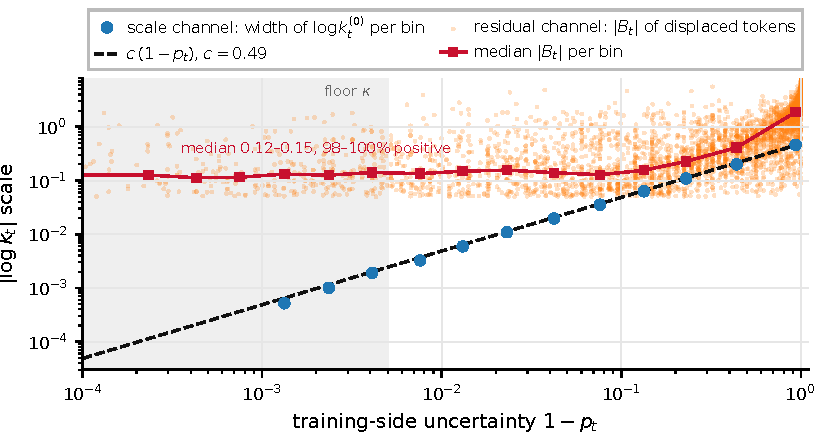
\includegraphics[width=0.5\textwidth]{figures/two_channel.pdf}
% % \vspace{-0.6\baselineskip}
% % \caption{Two channels on the same tokens (trained MoE, 509k tokens): the scale channel $|\log k_t|$ (blue) has width $\propto 1-p_t$; the residual $|B_t|$ (orange) does not scale and is almost entirely positive. Shaded: the floor $\kappa$. Details in \Cref{sec:exp_measurement}.}
% % \label{fig:two_channel}
% % \vspace{-0.8\baselineskip}
% % \end{wrapfigure}

% We measured $k_{i,t}$ systematically on large-scale rollouts; experimental
% details are given in \Cref{sec:exp_measurement}. Write
% $p_{i,t}=\pi_{\mathrm{train}}(y_{i,t}\mid x,y_{i,<t};\theta_{\mathrm{old}})$
% for the training-side probability of the token that was actually sampled, and
% drop the index $i$ in what follows. Two facts emerge
% (\Cref{fig:two_channel}). First, the conditional law of $\log k_t$ forms a
% \emph{scale family}, $\log k_t \,\big|\, p_t \overset{d}{=} c\,(1-p_t)\,Z$ with
% the law of $Z$ not depending on $p_t$, so that the shape is fixed and the width
% is proportional to $1-p_t$, where $c>0$ is a constant of the model and engine
% configuration. Second, a small fraction of tokens does not obey this law: their
% deviations do not scale with $1-p_t$, and their magnitude is set by router
% logit gaps and by the storage resolution of the log-probabilities. These two
% facts give the following model.

% \begin{definition}[Two-channel model]
% \label{def:two_channel}
% Conditionally on $p_t$, the observed log-ratio is generated as
% \begin{equation}
% \log k_t
% \;=\;
% c\,(1-p_t)\,Z_t
% \;+\;
% B_t ,
% \label{eq:two_channel}
% \end{equation}
% where the two components satisfy the following.

% \emph{(i) Scale component.} $Z_t\sim F_Z$ with $F_Z$ independent of $p_t$, and
% \begin{equation}
% \E[Z_t]=0,
% \qquad
% \E\abs{Z_t}<\infty,
% \qquad
% \E[(Z_t)_+]>0,
% \qquad
% z_{\min}(p_t)\le Z_t\le z_{\max}(p_t),
% \label{eq:scale_conditions}
% \end{equation}
% the endpoints of the support being induced by the constraint
% $p_t\le k_t\le 1/\pi_{\mathrm{infer}}(y_t)$. Beyond an upper tail that is
% generalized Pareto with shape $\xi_+\in(0,1)$ within that support, no
% parametric form is assumed for $F_Z$.

% \emph{(ii) Residual component.} $\Prob(B_t\ne0)\le\eps$, the event
% $\{B_t\ne0\}$ is independent of $(Z_t,p_t)$, and
% \begin{equation}
% -B_{\min}\le B_t\le B_{\max},
% \qquad
% B_{\min},B_{\max}\ \text{independent of}\ p_t;
% \qquad
% B_t\ge0
% \ \ \text{when}\ \
% 1-p_t\le\varphi_0 .
% \label{eq:residual_conditions}
% \end{equation}
% The value of $B_t$ within the envelope is left unmodeled.
% \end{definition}

% \subsection{Estimand and robust risk}
% \label{sec:robust_risk}

% The per-step change of measure
% $\E[k_t\,\ell'_t\mid h_t]=\E_{y_t\sim\pi_{\mathrm{train}}}[\ell'_t\mid h_t]$
% holds exactly at every prefix $h_t$; the question is not whether it is valid
% but which functional of the configuration we optimize. The two channels of
% \Cref{def:two_channel} differ on precisely this point. The scale channel is
% determined by $(c,F_Z)$: given a model and an engine configuration it is the
% same law on every batch. The residual channel is determined by which tokens
% happen to fall on a routing boundary or below the storage resolution, and is
% stable neither across batches nor across configurations; carrying it in the
% target would make the estimand move from batch to batch, and no threshold
% compiled from it would transfer. We therefore take the gradient induced by the
% scale channel alone,
% \begin{equation}
% G_0:=\E\big[e^{\,c(1-p_t)Z_t}\,\ell'\big],
% \label{eq:estimand}
% \end{equation}
% as the estimand; it coincides with $\E[k\,\ell']$ at $\eps=0$, and the residual
% becomes a nuisance---absent from the target, present in every sample.

% For a given sampling law $P$ the mean-squared error of the estimator is
% $\mathcal E_0(\Mclass;P)=\E_P\norm{\widehat G_{\Mclass}-G_0}^{2}$. It cannot be
% optimized directly: $B_t$ is characterized only at the level of sets and
% carries no law to integrate against. We therefore optimize
% \begin{equation}
% \mathcal E(\Mclass)
% :=
% \sup_{P\in\Uset}
% \left\{
% \Big(\sum_p\norm{b_p(\Mclass)}\Big)^{2}
% +\frac{1}{n}\E_P\big[\Mclass^{2}\norm{\ell'}^{2}\big]
% \right\},
% \label{eq:robust_risk}
% \end{equation}
% where
% $b_p(\Mclass)=\E\big[\big(\Mclass(k_t)-e^{\,c(1-p_t)Z_t}\big)\ell'_t\mid p_t=p\big]\,
% \Prob(p_t=p)$
% is the contribution of confidence level $p$ to the bias, and
% $\Uset=\big\{P:\ \log k_t=c(1-p_t)Z_t+B_t,\ Z_t\sim F_Z,\
% \Prob(B_t\ne0)\le\eps,\ -B_{\min}\le B_t\le B_{\max}\big\}$.

% \begin{theorem}[CIS operator, informal]
% \label{thm:cis_informal}
% Under \Cref{def:two_channel}, and when the displacement of the residual channel
% in standardized coordinates is sufficiently large, to first order on the log
% scale the minimizer of the robust risk over the shrinkage class is
% \begin{equation}
% \log\Mclass^{\star}(k_t,p_t)
% =
% \argminop_{\Mclass\in\Mdown}\mathcal E(\Mclass)
% =
% \min\Big(\log k_t,\;\lambda\,(1-p_t)\Big),
% \label{eq:cis_operator}
% \end{equation}
% where the slope is $\lambda=c\,\tau^{\star}$ and the threshold $\tau^{\star}$
% is uniquely determined by $F_Z$, the residual occurrence rate $\eps$, and the
% sample size $n$.
% \end{theorem}

% \subsection{The deployed algorithm}
% \label{sec:algorithm}

% \Cref{thm:cis_informal} gives a one-sided bound whose width scales with
% $1-p_t$. One correction is needed once $c(1-p_t)$ falls below the storage
% resolution of the log-probabilities: there the observed width of $\log k_t$
% saturates at that resolution rather than following $c(1-p_t)$, the two
% components of \eqref{eq:two_channel} cannot be separated in the data, and an
% unfloored band would truncate quantization noise rather than mismatch. We
% therefore floor the scale variable at $\kappa$, which gives \Cref{alg:cis}.
% The two hyperparameters admit measured defaults rather than a search:
% \Cref{thm:cis_informal} compiles $\lambda=c\,\tau^{\star}$, and $\kappa$ is the
% storage resolution of the log-probabilities.

% \begin{wrapfigure}{r}{0.5\textwidth}
% \vspace{-\baselineskip}
% \begin{minipage}{0.5\textwidth}
% \begin{algorithm}[H]
% \caption{Calibrated importance sampling (CIS)}
% \label{alg:cis}
% \begin{algorithmic}[1]
% \Require $\ell^{\mathrm{train}}_j$, $\ell^{\mathrm{infer}}_j$, $\ell'_j$ for
% the $n$ tokens of the batch; $\lambda$; $\kappa$
% \For{$j=1,\dots,n$}
%   \State $\log k_j\gets\ell^{\mathrm{train}}_j-\ell^{\mathrm{infer}}_j$,\quad
%   $p_j\gets\exp(\ell^{\mathrm{train}}_j)$
%   \State $w_j\gets\exp\big(\min\{\log k_j,\;
%   \lambda\max(1-p_j,\kappa)\}\big)$
% \EndFor
% \State \Return $\widehat G_{\mathrm{CIS}}
% =\frac{1}{n}\sum_{j=1}^{n}\operatorname{stopgrad}(w_j)\,\ell'_j$
% \end{algorithmic}
% \end{algorithm}
% \end{minipage}
% \end{wrapfigure}

% The operator adds one elementwise pass and no forward or backward computation.
% Three implementation details are load-bearing: the inference-side
% log-probability must be the raw value recorded at the sampling step, with no
% temperature rescaling or renormalization applied afterwards; the weight must be
% detached, since $k_t$ is data rather than a function of $\theta$; and the floor
% must be applied to $1-p_t$ before multiplication by $\lambda$, not to the
% resulting band.
\section{Experiments}
\label{sec:experiments}

The experiments answer five questions. \textbf{RQ1}: do logged rollouts support the two-channel model of \Cref{sec:two_channel}, and do the measured constants reproduce the predictions of \Cref{sec:cis}? \textbf{RQ2}: inside one RL system and under one recipe, does the deployed operator improve held-out accuracy and training stability over the cap, the gate, and the exact ratio? \textbf{RQ3}: which elements of the operator matter, and in which direction? \textbf{RQ4}: can the slope be compiled from measurements, and does the compiled slope transfer across serving configurations as the proportionality $\lambda_+=c\tau^\star$ of \Cref{thm:cis_informal} prescribes? \textbf{RQ5}: which tokens does the band act on during training? Section~\ref{sec:experiments-setup} describes the shared setup; each subsequent subsection answers one question. Implementation details and additional tables and figures are in Appendix~\ref{app:experimental}.

\subsection{Setup}
\label{sec:experiments-setup}

\noindent\textbf{Mismatch measurement.}\label{sec:exp_measurement}
We measure $(k_t,p_t)$ on 12.3M tokens of Qwen1.5-MoE-A2.7B-Chat and 12.4M tokens of a dense control (Qwen1.5-14B-Chat): vLLM samples eight responses per DAPO-Math prompt at temperature one and records each sampled token's log-probability at the sampling step, and the training engine rescores the same sequences at the same parameters. Controls, the paired stale-snapshot measurement behind Figure~\ref{fig:two_channel}, and training-time logging are in Appendix~\ref{app:experimental-diagnostics}.

\noindent\textbf{Training.}
We train Qwen1.5-MoE-A2.7B-Chat with AReaL on the GSM8K training set (SGLang rollouts, FSDP training, both bf16) and report greedy exact-match accuracy on the 1{,}319 held-out test problems (standard error about $1.3$ points per arm), with three seeds per method and one further run per method with the KV cache quantized to FP8. All arms share one recipe and code path (Appendix~\ref{app:experimental-implementation}) and differ only in the operator: no correction, the exact ratio, TIS (cap $2$), IcePop (mask $[0.5,5]$), the binary-KL mask of AReaL (KPop, threshold $2$), and CIS (\Cref{alg:cis}, $\lambda_+=2.3$, $\kappa=5\times10^{-3}$).

\subsection{RQ1: Do rollout logs support the two-channel model?}
\label{sec:experiments-diagnostics}

\begin{figure}[t]
\centering
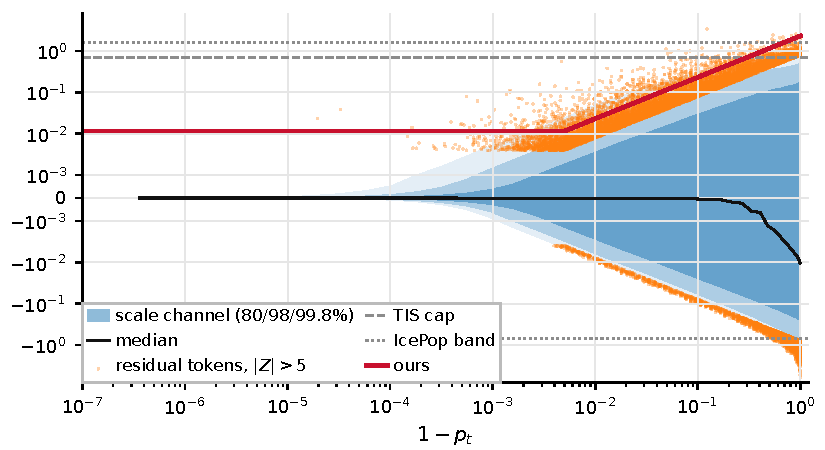
\includegraphics[width=\linewidth]{figures/mechanism.pdf}
\caption{Conditional distribution of $\log k_t$ against training-side uncertainty $1-p_t$ on the MoE model (12.3M tokens; symmetric-log vertical axis). Blue bands are the central 80\%, 98\%, and 99.8\% of tokens per uncertainty bin and follow the scale family of \Cref{def:two_channel} over six decades; the black line is the conditional median. Orange points are residual tokens with $|Z_t|>5$; at high confidence they lie above the shrinking bulk and are almost all positive. Grey lines are the constant thresholds of TIS ($\log 2$, dashed) and IcePop ($\log 0.5$ and $\log 5$, dotted), which lie above the entire distribution except at the least confident tokens. The red curve is the deployed one-sided band of \Cref{alg:cis}; its floor $\lambda_+\kappa=0.0115$ meets the residual layer at high confidence.}
\label{fig:mechanism}
\end{figure}

\noindent\textbf{Scale channel.}
Throughout this section $\varphi_t:=\max(1-p_t,\kappa)$ denotes the floored uncertainty of \Cref{alg:cis}, and $Z_t:=\log k_t/(c\varphi_t)$ the standardized deviation. Figure~\ref{fig:mechanism} shows the conditional distribution of $\log k_t$. Its width follows the scale family of \Cref{def:two_channel} across six decades of uncertainty, with $c=0.155$ for the MoE model and $c=0.035$ for the dense model and a weighted $R^2$ of $0.998$ over twenty equal-mass bins. After standardization by $c\varphi_t$ the central quantiles of $Z_t$ collapse across bins: between $\varphi=5\times10^{-3}$ and $\varphi=1$ the median moves by $0.06$ and the two deciles by $0.35$ and $1.17$ (Figure~\ref{fig:pivot}a). The upper tail is generalized Pareto with $\xi_+=0.49$ above the 99th percentile for the MoE model and $\xi_+=0.07$ for the dense model, so the MoE tail is heavy and some truncation is necessary rather than optional.

\noindent\textbf{Residual channel.}
We call a token residual when $|Z_t|>\zeta$ with the preregistered $\zeta=5$. Residual tokens are sparse, with $\hat\epsilon=1.26\%$ ($2.16\%$ at $\zeta=4$ and $0.78\%$ at $\zeta=6$), and their indicator is uncorrelated with $\varphi_t$ (correlation $0.004$). They cluster only weakly within trajectories: the lag-one autocorrelation of the indicator is $0.041$ against a permutation null of $0.0002$, and the conditional lift decays from $4.2$ at lag one to $2.6$ at lag four. At high confidence ($\varphi<0.05$) the residual displacement is one-sided, with $97.7\%$ of residual tokens positive on the base model and $100\%$ on the trained policy, and it is bounded, with a 99th percentile of $0.33$. Residual tokens are enriched in hard routing flips, which we define as a route change with gate margin above $10^{-3}$, by a factor of $1.46$ over the base rate of $0.53$, and they carry $2.0$ flipped layers on average against $1.1$ overall; the enrichment is real but not decisive, so routing is one contributor to the residual channel rather than its only cause. On the base model the residual median magnitude still scales with $\varphi$, at a fixed factor of about six above the bulk (Figure~\ref{fig:dualscale}a). The non-scaling behavior of \Cref{def:two_channel} appears once the policy has been trained and once the two engines are displaced in version. On the same tokens scored under a snapshot that is 29 steps stale, and in the logs of the training run itself, the residual magnitude at $\varphi<0.02$ lies between $0.04$ and $0.11$ while $c\varphi$ lies one to two orders of magnitude below it (Figure~\ref{fig:dualscale}b,c). We therefore state the non-scaling envelope as a high-confidence property, which is the regime in which \Cref{thm:cis_informal} is invoked. The paired measurement also fixes the sign structure of version displacement: rescoring the same tokens under the same snapshot through the two decode paths gives exactly zero difference, the displacement between snapshots is two-sided overall ($48.9\%$ positive) with a negative median at low confidence which reflects policy sharpening, and it is entirely positive on the high-confidence residual tokens that the operator acts on.

\noindent\textbf{Null measurements on the $\epsilon=0$ section.}
When $\epsilon=0$ the robust risk~\eqref{eq:robust_risk} reduces to an average-case criterion, and such criteria do not produce a confidence-dependent band; the band is a consequence of $\epsilon>0$. Four independent measurements on the same logs agree with this prediction. The sequence-level surface $\Delta(\varphi)$ has slope $-0.002$ with a trajectory-bootstrap interval of $[-0.48,0.15]$ over $20{,}000$ trajectories; the coupling coefficient $\lambda_{\mathrm{eff}}=c(\beta_1-\tfrac32\beta_2)$ has an interval which covers zero in three independent batches; the bare leave-one-out sum has slope $0.31$ against $\varphi$, of which $0.25$ survives a permutation that destroys within-trajectory coupling; and best-response iteration of the sequence-level risk converges from every start to a constant cap with $\lambda^\star=0.07$. The cross-layer coherence check gives a far-layer gradient coherence of $0.10$ between confidence layers, which is indistinguishable from its permutation null, and within a layer the token gradient directions are nearly orthogonal ($\rho\approx0.005$). RQ1 is therefore answered in the affirmative for the scale channel and for the sparsity, sign, and boundedness of the residual channel, with the qualification that the non-scaling envelope is a high-confidence property.

\subsection{RQ2: Does the operator improve accuracy and stability over the cap and the gate?}
\label{sec:experiments-results}

\begin{table}[t]
\centering
\caption{Held-out GSM8K accuracy (\%) after three epochs with three seeds per method, same recipe and code path for all methods; the untrained model scores $52.31$. Training reward is the mean over the third epoch, and intervened tokens is the fraction of loss tokens that the operator truncated or masked, both for seed one and as reported by the training framework. All methods take $31$ to $34$ seconds per optimizer step on the same hardware; no operator adds a forward or backward pass. The three leading methods lie within one standard error of one another; the deployed operator has the highest mean, the smallest spread, and the highest worst seed.}
\label{tab:main}
\small\setlength{\tabcolsep}{4pt}
\begin{tabular}{lcccccc}
\toprule
Method & Seed 1 & Seed 2 & Seed 3 & Mean $\pm$ std & Train reward & Intervened (\%) \\
\midrule
No correction ($M\equiv1$) & 56.10 & 54.44 & 56.10 & $55.55\pm0.96$ & 0.73 & 0 \\
Exact ratio ($M=k$) & 64.59 & 55.50 & 59.06 & $59.72\pm4.58$ & 0.843 & 0 \\
KPop (binary-KL mask, $2$) & 59.44 & 59.29 & 57.85 & $58.86\pm0.88$ & 0.852 & 21.9 \\
IcePop (mask $[0.5,5]$) & \textbf{64.82} & 62.70 & 63.46 & $63.66\pm1.07$ & 0.855 & 4.1 \\
TIS (cap $2$) & 62.40 & 63.91 & \textbf{65.43} & $63.91\pm1.52$ & 0.847 & 0.8 \\
CIS (ours, \Cref{alg:cis}) & 64.67 & \textbf{64.97} & 63.23 & $\mathbf{64.29\pm0.93}$ & \textbf{0.867} & 4.2 \\
\bottomrule
\end{tabular}
\end{table}

\begin{figure}[t]
\centering

\includegraphics[width=0.9\linewidth]{figures/dyn_legend.pdf}\\[2pt]
\begin{minipage}[t]{0.325\linewidth}\centering
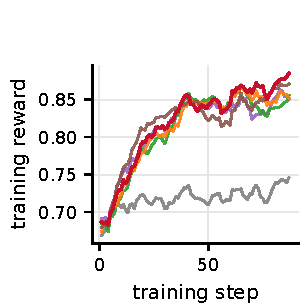
\includegraphics[width=\linewidth]{figures/dyn_reward.pdf}\\[-2pt]{\small (a)}
\end{minipage}\hfill
\begin{minipage}[t]{0.325\linewidth}\centering
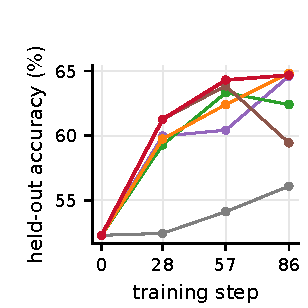
\includegraphics[width=\linewidth]{figures/dyn_heldout.pdf}\\[-2pt]{\small (b)}
\end{minipage}\hfill
\begin{minipage}[t]{0.325\linewidth}\centering
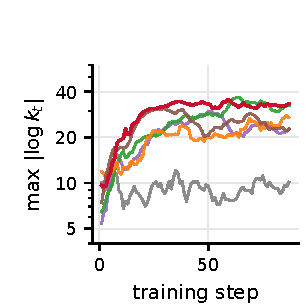
\includegraphics[width=\linewidth]{figures/dyn_gapmax.pdf}\\[-2pt]{\small (c)}
\end{minipage}\\[4pt]
\begin{minipage}[t]{0.325\linewidth}\centering
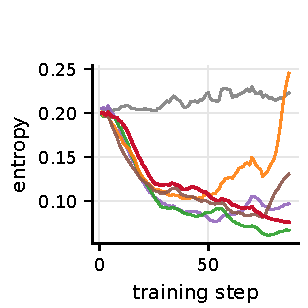
\includegraphics[width=\linewidth]{figures/dyn_entropy.pdf}\\[-2pt]{\small (d)}
\end{minipage}\hfill
\begin{minipage}[t]{0.325\linewidth}\centering
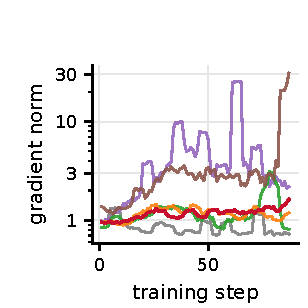
\includegraphics[width=\linewidth]{figures/dyn_grad.pdf}\\[-2pt]{\small (e)}
\end{minipage}\hfill
\begin{minipage}[t]{0.325\linewidth}\centering
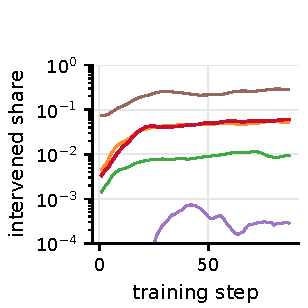
\includegraphics[width=\linewidth]{figures/dyn_rs.pdf}\\[-2pt]{\small (f)}
\end{minipage}
\caption{Training dynamics of the six operators under one recipe (seed one; curves smoothed over five steps). (a) Training reward. (b) Held-out accuracy of the epoch checkpoints, starting from the untrained model: the deployed operator leads at every checkpoint ($61.3$, $64.3$, $64.7$), and the KL mask peaks at $63.8$ after two epochs and falls to $59.4$ in the last one. (c) Largest $|\log k_t|$ in the batch, which grows during training for every corrected run as the policy sharpens. (d) Policy entropy. (e) Gradient norm: the exact ratio is spiky and the KL mask diverges late, whereas the cap, the gate, and the band stay near one. (f) Fraction of loss tokens intervened on by each operator; the KL mask removes about a fifth of all tokens.}
\label{fig:dynamics}
\end{figure}

Table~\ref{tab:main} reports held-out accuracy for six operators applied to the same pair $(k_t,p_t)$ in the same code, and Figure~\ref{fig:dynamics} shows their training dynamics. Correcting the mismatch in any bounded way adds $8.7$ points over the uncorrected loss, whose training reward stalls at $0.73$ while every corrected run climbs to about $0.85$. Among the corrections, the deployed operator has the highest mean, the smallest spread across seeds, and the highest worst seed, and it also has the highest training reward. The three leading methods lie within one standard error of one another, so we do not claim a significant ordering among them on this task and model. The dynamics separate the methods more clearly than the endpoints. On the held-out checkpoints (Figure~\ref{fig:dynamics}b) the deployed operator is ahead at every epoch, and it is the only method whose accuracy does not dip in any epoch. The exact ratio has a healthy reward curve on every seed but a gradient norm which spikes to ten and a held-out spread of $9.1$ points, and on seed two it falls to the level of no correction while its training reward stays close to the other seeds. The KL mask has the highest intervention rate, about $22\%$ of loss tokens, and its gradient norm diverges in the last epoch. On inspection, this rate is a numerical property of the Bernoulli-KL metric rather than a property of the KL threshold: in single precision the clamp bound $1-10^{-8}$ equals one, so a token whose probability is exactly one on either engine yields an infinite or undefined metric and is masked; these are $19\%$ of tokens, all at the highest confidence, and they account for the intervention rate. We report the framework's implementation as run; a numerically corrected variant, which computes the metric in double precision and treats the saturated case as zero divergence, scores $61.03\pm2.24$ over three seeds (Appendix~\ref{app:experimental-results}), above the implementation as shipped but still below the cap, the gate, and the band. Held-out accuracy and training reward disagree in several places in Table~\ref{tab:main} and in the ablations that follow; whenever they disagree, the training reward is the quantity that is blind to the difference.

\subsection{RQ3: Which elements of the operator matter, and in which direction?}
\label{sec:experiments-analysis}

\begin{table}[t]
\centering
\caption{Single-variable ablations of the deployed operator (seed one unless stated). Each row changes one element of \Cref{alg:cis}. Lifting the lower side and raising the floor leave the training reward unchanged or higher while lowering held-out accuracy; the row in bold reaches the highest training reward of the study and the held-out accuracy of no correction.}
\label{tab:ablation}
\small
\begin{tabular}{llcc}
\toprule
Element & Variant & Held-out (\%) & Train reward \\
\midrule
Deployed & $\lambda_-=\infty$, $\lambda_+=2.3$, $\kappa=5\times10^{-3}$ & 64.67 & 0.867 \\
Lower side & lift to $w\ge0.001$ & 63.15 & 0.851 \\
Lower side & \textbf{lift to $w\ge0.1$} & \textbf{56.10} & \textbf{0.878} \\
Lower side & symmetric band, $\lambda_-=1.0$ & 48.98 & 0.827 \\
Floor & none ($\kappa\to0$) & diverged at step 79 & --- \\
Floor & $\kappa=0.1$ (three seeds) & $61.01\pm0.83$ & 0.857--0.877 \\
Band shape & affine, $+0.12$ added to the band & 62.85 & 0.838 \\
Slope & $\lambda_+=0.9$ (compiled, Table~\ref{tab:compile}) & 64.44 & 0.868 \\
Slope & $\lambda_+=1.6$ & 64.67 & 0.859 \\
Slope & $\lambda_+=3.1$ & 63.76 & 0.861 \\
\bottomrule
\end{tabular}
\end{table}

\noindent\textbf{One-sidedness and dose response.}
Table~\ref{tab:ablation} varies one element of the operator at a time. Lifting the lower side degrades held-out accuracy monotonically with the amount of lifting: from $64.67$ with no lower bound to $63.15$ at $w\ge0.001$, to $56.10$ at $w\ge0.1$, and to $48.98$ for the symmetric band, which is below the untrained model. The training reward does not register this harm; the $w\ge0.1$ variant reaches the highest training reward of the entire study while its held-out accuracy returns to the uncorrected level. An intermediate checkpoint of that run scores $62.62$ after one epoch and $56.10$ after three, so the harm accumulates as the policy sharpens and more tokens fall into the lifted region. Together with the support bound $k_t\ge p_t$, this is the empirical basis for restricting to the shrinkage class $\Mdown$ of \Cref{sec:prelim_estimation}.

\noindent\textbf{Floor, band shape, and slope.}
Without a floor the band collapses at high confidence: in the third epoch $32\%$ of tokens are truncated, the truncated tokens have median $|\log k_t|=7\times10^{-4}$, which is the resolution of the stored log-probabilities, and training diverges at step 79. With $\kappa=5\times10^{-3}$ the truncated tokens have median $|\log k_t|$ between $0.08$ and $0.12$. Raising the floor to $\kappa=0.1$, which places $58\%$ of tokens under a constant cap of $0.23$, costs $3.3$ points on three seeds while leaving the training reward unchanged; the floor is the storage resolution, not the residual scale. Adding a constant $0.12$ to the band costs $1.8$ points, which agrees with the null measurements of Section~\ref{sec:experiments-diagnostics}: the data support a multiplicative band and do not support additive widening. The slope is robust on the plateau $\lambda_+\in\{0.9,1.6,2.3\}$, where the three values score $64.44$, $64.67$, and $64.67$, and it declines slightly at $3.1$. RQ3 is answered as follows: the lower side must be left open, the floor must sit at the storage resolution, the band must scale multiplicatively with $\varphi_t$, and the slope is insensitive within a factor of two and a half.

\subsection{RQ4: Can the slope be compiled, and does it transfer across serving configurations?}
\label{sec:experiments-transfer}

\begin{table}[t]
\centering
\caption{The compilation chain of \Cref{thm:cis_informal}. Every input is measured without a training run; the output is compared with the slope that the RL sweep selects. The exceedance check compares $\Pr(Z>\lambda_+/c)$ at the deployed slope with the independently measured version-staleness rate. The FP8 row applies the proportionality rule to a changed serving configuration.}
\label{tab:compile}
\footnotesize\setlength{\tabcolsep}{3.5pt}
\begin{tabular}{lcccccc}
\toprule
Configuration & $c$ & $\xi_+$ & $\hat\epsilon$ & $\tau^\star$ & $\lambda_+=c\tau^\star$ & RL optimum / outcome \\
\midrule
bf16, base model & 0.155 & 0.49 & 0.0176 & 5.7 & 0.9 & 64.44 at 0.9; plateau $\{0.9,1.6,2.3\}$ \\
bf16, early training & 0.61 & --- & --- & 5.7 & 3.5 & deployed 2.3 in between \\
Exceedance check & \multicolumn{6}{l}{$\Pr(Z>\lambda_+/c)=0.13\%$ vs.\ staleness rate $0.5$--$0.6\%$ (same order)} \\
FP8 KV cache & 1.75 & --- & --- & --- & $2.3\times2.9=6.7$ & 63.00 vs.\ 60.12 at 2.3 \\
\bottomrule
\end{tabular}
\end{table}

\begin{table}[t]
\centering
\caption{Held-out accuracy (\%) with the SGLang KV cache quantized to FP8, seed one. Quantization raises the training-time scale constant from $c=0.60$ to $c=1.75$ on tokens generated and scored at the same parameter version. Rescaling the slope by that ratio recovers most of the loss; halving the adjustment does not.}
\label{tab:fp8}
\small
\begin{tabular}{lccc}
\toprule
Method & bf16 & FP8 KV cache & Change \\
\midrule
No correction & 56.10 & 54.36 & $-1.7$ \\
Exact ratio & 64.59 & 57.62 & $-7.0$ \\
KPop & 59.44 & 50.19 & $-9.3$ \\
IcePop & 64.82 & \textbf{63.84} & $-1.0$ \\
TIS & 62.40 & 60.20 & $-2.2$ \\
Ours, $\lambda_+=2.3$ (bf16 slope) & 64.67 & 60.12 & $-4.6$ \\
Ours, $\lambda_+=4.0$ & 64.67 & 59.82 & $-4.9$ \\
Ours, $\lambda_+=6.7$ (rescaled by $c_{\mathrm{FP8}}/c_{\mathrm{bf16}}=2.9$) & 64.67 & 63.00 & $-1.7$ \\
\bottomrule
\end{tabular}
\end{table}

\noindent\textbf{Compilation.}
Table~\ref{tab:compile} runs the compilation chain of \Cref{thm:cis_informal} on the measured constants. With $\hat\epsilon=1.76\%$ measured off the quantization floor and the empirical $F_Z$, the equalizer condition that fixes $\tau^\star$ in \Cref{thm:cis_informal}, $H(\tau)/\tau=\epsilon/(2-\epsilon)$ with $H(\tau)=\E[(Z-\tau)_+]$, has the root $\tau^\star=5.7$, which lies at the knee where the standardized bulk turns into the Pareto tail (Figure~\ref{fig:pivot}b,c). At the base-model scale this compiles to $\lambda_+=0.9$. The scale constant grows during training, from $0.16$ on the base model to $0.61$ in the first third of the run and $1.67$ in the last third, so the same $\tau^\star$ compiles to $3.5$ at the early-training scale. The deployed slope $\lambda_+=2.3$ lies between these two values. Running the compiled value itself gives $64.44$, which is on the same plateau as $1.6$ and $2.3$ ($64.67$ each), so the chain lands on the held-out optimum without any tuning, and the two compilations bracket the deployed slope in the direction in which $c$ moves during training. The exceedance check of the corollary also passes: at the deployed slope, $\Pr(Z>\lambda_+/c)=0.13\%$ against a version-staleness rate of $0.5$ to $0.6\%$ in the training logs, which is the same order of magnitude.

\noindent\textbf{Transfer across serving configurations.}
Table~\ref{tab:fp8} tests the proportionality prediction directly. Quantizing the KV cache raises the training-time scale constant, measured on tokens generated and scored at the same parameter version, from $0.60$ to $1.75$, and it raises the fraction of such tokens truncated by the bf16 slope from $1.8\%$ to $5.2\%$. With the bf16 slope the operator loses $4.6$ points. Rescaling the slope by the measured ratio $2.9$ recovers $2.9$ of these points and brings the operator within one standard error of IcePop, whereas an intermediate slope of $4.0$ recovers nothing. Two baselines behave differently: the ratio mask of IcePop is nearly unaffected by quantization, and the KL mask falls below the untrained model, which is consistent with the saturation artifact described in Section~\ref{sec:experiments-results} becoming more frequent under quantization. Under the same conditions the uncorrected run collapses in the middle of training. The comparison is single-seed and we report it as such. RQ4 is answered as follows: the chain compiles a slope which sits on the RL optimum plateau, and the proportionality rule transfers the slope across serving configurations.

\subsection{RQ5: Which tokens does the band act on?}
\label{sec:experiments-trigger}

\begin{figure}[t]
\centering
\begin{minipage}[t]{0.325\linewidth}\centering
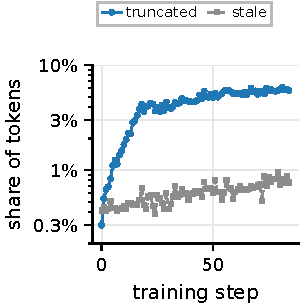
\includegraphics[width=\linewidth]{figures/trigger_a.pdf}\\[-2pt]{\small (a)}
\end{minipage}\hfill
\begin{minipage}[t]{0.325\linewidth}\centering
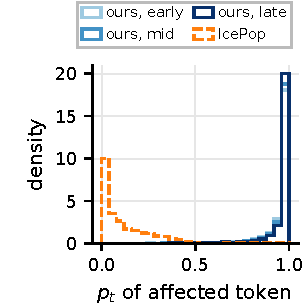
\includegraphics[width=\linewidth]{figures/trigger_b.pdf}\\[-2pt]{\small (b)}
\end{minipage}\hfill
\begin{minipage}[t]{0.325\linewidth}\centering
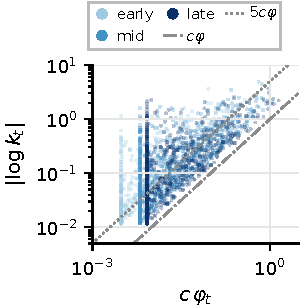
\includegraphics[width=\linewidth]{figures/trigger_c.pdf}\\[-2pt]{\small (c)}
\end{minipage}
\caption{What the band acts on during training (deployed operator, seed one; tokens logged every ten optimizer calls). (a) Fraction of truncated tokens per step (blue) and share of tokens whose rollout version is behind the current one (grey): the trigger rate rises from $0.3\%$ to about $5.5\%$ over the first forty steps and then stays flat, one order of magnitude above the stale share. (b) Training-side confidence $p_t$ of the affected tokens: the truncated tokens of our operator in the early, middle, and late third of training (blue, light to dark) concentrate at $p_t\to1$, whereas the tokens masked by IcePop in its own run (orange, dashed) concentrate at $p_t\to0$; the two operators act on complementary populations. (c) Magnitude $|\log k_t|$ of truncated tokens against the scale-channel width $c\varphi_t$ of their training phase, with $c$ fitted per phase; the dash-dotted and dotted lines mark $c\varphi_t$ and $5c\varphi_t$. Truncated tokens sit at $4$ to $7$ times the local width (median), and the vertical columns at the left are tokens on the floor $\varphi_t=\kappa$.}
\label{fig:trigger}
\end{figure}

Figure~\ref{fig:trigger} shows what the band does over the course of training. The trigger rate rises from $0.3\%$ to about $5.5\%$ during the first forty steps and then plateaus, one order of magnitude above the share of version-stale tokens, which stays between $0.4\%$ and $0.9\%$. Between $87\%$ and $90\%$ of the truncated tokens have $1-p_t<0.1$, and their median $|\log k_t|$ is $0.09$ to $0.10$ in every phase, which is $4$ to $7$ times the scale-channel width of that phase. In standardized training-time units, $49\%$ of the truncated tokens exceed $\zeta=5$ at $\lambda_+=2.3$ and $93\%$ do at $\lambda_+=6.7$, and among the truncated tokens the share of version-stale tokens is $3.0\%$, five times its base rate. Panel (b) is the clearest statement of the difference between the two operators: IcePop removes low-confidence tokens whose ratio leaves a fixed interval, and the band truncates high-confidence tokens whose displacement is large relative to their local width; the acceptance regions of all four operators are drawn in Figure~\ref{fig:regions} of the appendix. Panels (a) and (c) also record a fact about the training run itself: the scale constant grows from $0.61$ to $1.67$ between the first and last third of training while the width at high confidence stays small, so a slope calibrated on the base model becomes tighter in standardized units as training proceeds. This is the mechanism behind the FP8 result and the reason that the compilation $\lambda_+=c\tau^\star$ should be applied to the serving configuration at hand.

\section{Related Work}
\label{sec:related}

% \paragraph{Training--inference mismatch in language-model RL.}
% Current post-training pipelines split rollout generation and gradient computation across two engines. Inference systems such as vLLM and SGLang optimize throughput with paged attention, continuous batching, and fused kernels \citep{kwon2023vllm,zheng2024sglang}, whereas training systems such as FSDP or Megatron recompute log-probabilities with different kernels, reduction orders, and parallel layouts. The two realizations disagree even at identical parameters, and the disagreement depends on batch composition and decode path rather than being a fixed rounding offset \citep{he2025nondeterminism}. \citet{yao2025tis} show that this discrepancy turns nominally on-policy training into off-policy training and propose truncated importance sampling on the engine ratio. The Ring-1T report introduces IcePop, which zeroes tokens whose ratio leaves a fixed interval, and documents compounding mismatch over long runs together with sensitivity to the interval \citep{ling2025ring}. Systems-level remedies act on the source: FP16 arithmetic reduces the numerical discrepancy \citep{qi2025fp16}, Rollout Routing Replay reuses inference-time expert routes on the training side \citep{ma2025r3}, and DRPO replaces hard masking with a smooth divergence penalty \citep{yao2026drpo}. GSPO moves the correction unit from tokens to sequences \citep{zheng2025gspo}. Asynchronous systems such as AReaL add a second source of displacement, because a rollout may be scored by a parameter snapshot that is several versions newer than the snapshot which generated it \citep{fu2025areal}. We do not propose a new systems control. We ask which token-level operator is justified once the mismatch has been measured, and we evaluate the resulting operator against the cap and the gate inside one training system.

% \paragraph{Mixture-of-experts routing.}
% Sparse expert models route each token to a top-$k$ subset of experts through a learned gate \citep{fedus2022switch}. The routing decision is discrete, so a small perturbation of the gate logits can change which experts process a token, and the training engine may then score a token on experts that did not generate it \citep{ma2025r3,ling2025ring}. Our measurements treat this event as one source of a residual component of the mismatch, and we quantify how strongly it is enriched among large deviations.

% \paragraph{Importance weighting and truncation in off-policy RL.}
% Truncated importance sampling trades a controlled bias for bounded variance \citep{ionides2008truncated}. In deep RL the same device appears as the truncated traces of Retrace and the clipped weights of V-trace, both of which cap per-step ratios at a constant \citep{munos2016retrace,espeholt2018impala}. PPO and its group-relative variant GRPO handle parameter drift with a clipped surrogate rather than with an importance weight \citep{schulman2017ppo,shao2024deepseekmath}, and DAPO decouples the two clip ranges \citep{yu2025dapo}. All of these operators use a threshold which does not depend on the token. The operator studied here differs in that its threshold follows the measured conditional width of the mismatch.

% \paragraph{Robust statistics and robust RL.}
% Huber's contamination model and the associated minimax theory formalize a small fraction of arbitrary deviations \citep{huber1964robust,huber1965robust,huber1973minimax}, and CVaR admits a density-bounded dual representation \citep{rockafellar2000cvar}. In reinforcement learning, value clipping can be the exact image of a robust Bellman problem under total-variation geometry \citep{liu2026clipped}, and a line of work relates robustness to regularization and to divergence-structured robust MDPs \citep{derman2021twice,yang2023rmdp,zhang2024soft,tang2025f}. \citet{shi2023distributionally} organize KL-robust offline RL around an explicit nominal functional and a matching hard instance. We adopt the same discipline of deriving the exact population operator first and then exhibiting the class members which attain its constant. Classical robust testing distinguishes censoring from trimming, but it does not model a gradient payload whose computational path can be wrong. We encode that possibility as an unknown corrupted payload mean without a zero-mean assumption.


% % ============================================================
% % Sections 3-4: Preliminaries and Theoretical Framework
% % Environments assumed: assumption, definition, lemma, theorem,
% %   corollary, remark  (via amsthm)
% % Macros assumed: \E (\mathbb E), \R (\mathbb R); otherwise standard.
% % Proofs deferred to Appendix~\ref{app:proof}.
% % ============================================================


\label{sec:conclusion}

% Token-level ratio operators encode assumptions about an observation-law class. The bounded-band theorem gives capping both a population origin and an exact validity boundary. The localized-corruption theorem shows that gating is not uniformly justified without localization; once the nuisance support is localized, the exact solution is an identity-plus-clean-tail cap, and IcePop is the sharp zero-cap phase selected by a necessary-and-sufficient mass condition. In both cases, attaining members match the upper guarantees exactly. The remaining empirical question is which class is supported by rollout logs in a given model and system regime.

% Uncomment and complete the required disclosure before submission.
% \subsection*{AI Use Statement}
% Generative AI tools were used for language editing, structural organization,
% and LaTeX drafting. The authors verified the mathematical arguments,
% citations, and final claims and take responsibility for the manuscript.


\bibliography{iclr2027_conference}
\bibliographystyle{iclr2027_conference}
\appendix
\appendix
% ============================================================
% Appendix: proofs
% Requires the macros of the main file:
%   \E \Prob \norm \abs \Mclass \Mdown \Uset \eps \argminop
% ============================================================

% ============================================================
% Appendix: Proofs for the CIS Framework
% Requires macros from the main text:
% \E \Prob \norm \abs \Mclass \Mdown \Uset \eps
% ============================================================

% ============================================================
% Appendix: Proofs for the CIS Framework
% Requires macros from the main text:
%   \E \Prob \norm \abs \Mclass \Mdown \Uset \eps \argminop
% ============================================================
\clearpage
\section*{Appendix}

\startcontents[appendix]
\printcontents[appendix]{}{1}{\setcounter{tocdepth}{2}}

\vspace{1em}
% ============================================================
% Appendix A.1 -- Preliminaries and Key Lemmas  (ICPO-style proofs)
% Requires per-section numbering, e.g. \counterwithin{equation}{section}
% ============================================================
% ---------------------------------------------------------------------------
% Appendix: where the mismatch comes from.
% Referenced from Section 3.1 ("A detailed analysis is given in ...") -> app:mismatch
% and from Section 3.2 ("details are given in ...")                  -> app:mgf
% Figures: fig_app_grid.pdf, fig_app_routing.pdf
% Every number is measured; the only data are the two measurements of
% Appendix B.1 and the logit dump described in the first subsection.
% ---------------------------------------------------------------------------
\section{Where the Mismatch Comes From}
\label{app:mismatch}

\Cref{sec:logit_model} traces the displacement $\varepsilon_t$ to the
per-logit perturbation $\boldsymbol\delta$ through \eqref{eq:eps_identity}, and
\Cref{sec:why_correction} uses the moments of $e^{\varepsilon_t}$. This
appendix supplies the measurements behind both. We first measure
$\boldsymbol\delta$ directly (\Cref{app:mm-measure}). We then identify the two
mechanisms that produce its body and its tail (\Cref{app:mm-mechanisms}).
Finally, we show how the moments of $e^{\varepsilon_t}$ reported in
\Cref{fig:mgf} are assembled from these two components (\Cref{app:mgf}).

% ---------------------------------------------------------------------------
\subsection{Measuring the per-logit perturbation}
\label{app:mm-measure}

\paragraph{Gauge.}
The perturbation enters \eqref{eq:eps_identity} only through contrasts. Since
$\sum_{j\neq y_t}w_j=1$, shifting every coordinate by a constant $c$ leaves
the displacement unchanged:
$-(\delta_{y_t}+c)+\log\sum_{j\neq y_t}w_je^{\delta_j+c}=\varepsilon_t$.
The raw logit vectors of the two engines are therefore defined only up to a
per-position constant. We fix this freedom by working in the log-probability
gauge,
\begin{equation}
\delta_j\;=\;\log\pi_{\mathrm{infer}}(j\mid h_t)-\log\pi_{\mathrm{train}}(j\mid h_t),
\label{eq:delta_gauge}
\end{equation}
which differs from $\boldsymbol\delta$ in \eqref{eq:engine_logits} by a
constant. In this gauge, $\boldsymbol\delta$ is uniquely determined and
directly observable.

\paragraph{Protocol.}
The measurement of \Cref{app:diagnostics} records only the probabilities of the
\emph{sampled} token. To observe $\boldsymbol\delta$ itself, we select 250
trajectories and 24 generation positions per trajectory at random, for each
model. At each (trajectory, position) pair we dump the top-256 pre-softmax
logits of the training engine together with $\log\sum_je^{z_j}$, and the
next-token log-probabilities of the inference engine. The inference side is
obtained by truncating the sequence at the position and generating a single
token, which returns exactly the distribution at that position.
\texttt{prompt\_logprobs} is not used, since it materialises one dictionary per
position and does not fit in memory at this vocabulary size. Engine settings,
precision and controls are those of \Cref{app:diagnostics}. Rows align on
$100\%$ of pairs, and the top-256 sets of the two engines intersect on $0.950$
(MoE) and $0.989$ (dense) of their entries. The procedure costs eight
GPU-minutes per model and yields $1{,}457{,}477$ (MoE) and $1{,}521{,}672$
(dense) paired values of $\delta_j$ on the base checkpoints.

\begin{table}[t]
\centering
\caption{The per-logit perturbation $\delta_j$ on the base checkpoints, in the
gauge \eqref{eq:delta_gauge}. Both are centred. The dense control is bounded,
whereas on the MoE the body is $4.2\times$ wider and the tail reaches an order
of magnitude further.}
\label{tab:delta_stats}
\begin{tabular}{lcc}
\toprule
 & dense control & MoE \\
\midrule
paired entries              & $1{,}521{,}672$ & $1{,}457{,}477$ \\
mean / median               & $+0.0013$ / $0.0000$ & $+0.0036$ / $0.0000$ \\
mean / standard deviation   & $1.6\%$   & $1.1\%$ \\
standard deviation          & $0.079$   & $0.336$ \\
$\Pr(|\delta_j|>0.5)$       & $0.003\%$ & $9.87\%$ \\
$\Pr(|\delta_j|>1)$         & $0\%$     & $1.52\%$ \\
$\max_j|\delta_j|$          & $1.00$    & $10.47$ \\
\bottomrule
\end{tabular}
\end{table}

\paragraph{Result.}
\Cref{tab:delta_stats} summarises the measurement, and
\Cref{fig:mismatch}(b) plots the two distributions. On both architectures the
perturbation is centred: its mean is $1$--$2\%$ of its standard deviation,
and its median is zero to the resolution of the measurement. The two
architectures differ in the tail. On the dense control, no entry exceeds
$|\delta_j|=1$ in $1.5$M draws. On the MoE, $1.52\%$ of entries exceed $1$ and
the largest reaches $10.47$. The split into a bulk $F_0$ and a residual
$G_{p_t}$ in \Cref{def:logit_displacement} is therefore already visible at the
level of $\boldsymbol\delta$, before \eqref{eq:eps_identity} maps it to
$\varepsilon_t$.

% ---------------------------------------------------------------------------
\subsection{Two mechanisms: rounding and routing}
\label{app:mm-mechanisms}

\begin{figure}[t]
\centering
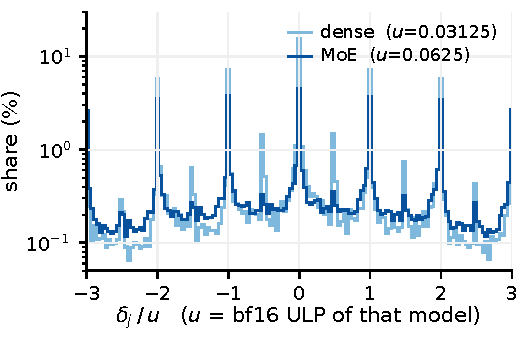
\includegraphics[width=0.62\linewidth]{figures/fig_app_grid.pdf}
\caption{$\delta_j$ in units of the bf16 unit in the last place $u$ at each
model's logit magnitude ($u=2^{-5}$ for the dense control, $u=2^{-4}$ for the
MoE). Mass concentrates on the integers, that is, on the representable grid.
Bin width $u/25$; log vertical axis.}
\label{fig:app_grid}
\end{figure}

\paragraph{Rounding produces the bulk.}
If the body of $\boldsymbol\delta$ were bf16 rounding error, its values would
concentrate on the representable grid, and they do. At logit magnitude $|z|$
the grid spacing is $u=2^{\lfloor\log_2|z|\rfloor-7}$. This gives $u=2^{-5}$
for the dense control (root-mean-square $|z|=7.6$) and $u=2^{-4}$ for the MoE
($|z|=11.4$). Measured in these units, $61.8\%$ of dense entries and $50.8\%$ of
MoE entries lie within $0.05$ of an integer, against $10\%$ under a uniform
phase. \Cref{fig:app_grid} shows the resulting comb.

The grid can also be recovered from the data alone. For the dense model, the
fraction of entries within $0.1$ of a grid point is $67.9\%$ at spacing
$2^{-5}$, $46.6\%$ at $2^{-4}$ and $32.0\%$ at $2^{-3}$. For the MoE it is
$57.8\%$ and $58.7\%$ at $2^{-5}$ and $2^{-4}$, and $36.4\%$ at $2^{-3}$. In both
cases, the coarsest spacing that retains the concentration is the one
predicted by the model's own logit magnitude.

The rounding model also predicts the \emph{size} of the bulk. Write
$\delta_j=\nu_j|z_j|$, with $\nu_j$ zero-mean, independent of $z$, and bounded
by the bf16 unit roundoff $u_0=2^{-8}$, so that $\sigma_\nu=u_0/\sqrt3$. A
first-order expansion of \eqref{eq:eps_identity} gives
$\operatorname{Var}(\varepsilon_t)\approx\sigma_\delta^2(1+\sum_jw_j^2)$.
Under a Gaussian approximation this yields
$\mu\approx\exp(\operatorname{Var}(\varepsilon_t)/2)$. \Cref{tab:rounding}
compares this prior, which is not fitted to $\boldsymbol\delta$, with the
measurement. On the dense control, where there is no routing, both the
prediction and the measurement are indistinguishable from $\mu=1$. On the MoE,
the prediction falls short by two orders of magnitude on the base checkpoint
and by four on the trained one. Rounding therefore accounts for the bulk, and
a second mechanism is needed for the rest.

\begin{table}[t]
\centering
\caption{Rounding-model prior against measurement. The prior uses only the bf16
unit roundoff and the measured logit magnitudes.}
\label{tab:rounding}
\begin{tabular}{lcccc}
\toprule
 & rms $|z|$ & $\sigma_\delta$ (prior) & $\mu-1$ (prior) & $\mu-1$ (measured) \\
\midrule
dense control, base    & $7.6$  & $0.017$ & $0.00023$ & $-0.0016$ \\
MoE, base              & $11.4$ & $0.025$ & $0.00049$ & $+0.042$ \\
MoE, trained (step 86) & ---    & ---     & $0.00049$ & $+6.07$ \\
\bottomrule
\end{tabular}
\end{table}

\begin{figure}[t]
\centering
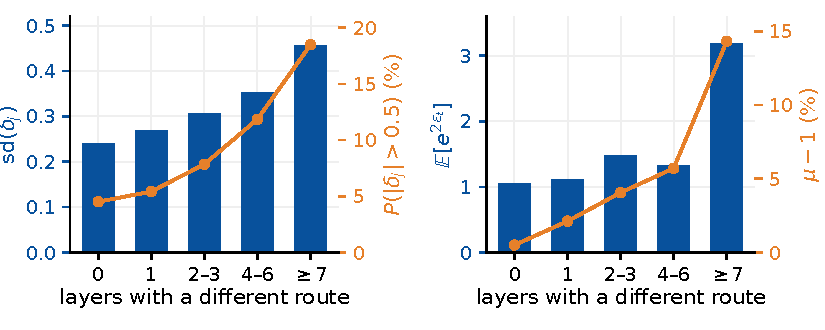
\includegraphics[width=\linewidth]{figures/fig_app_routing.pdf}
\caption{Routing disagreement between the two engines on the base MoE. Left:
width of $\delta_j$ (bars) and its tail mass (line). Right: second moment of
$e^{\varepsilon_t}$ (bars) and $\mu-1$ (line). All four quantities grow with the
number of layers at which the two engines select different experts.}
\label{fig:app_routing}
\end{figure}

\paragraph{Routing modulates the tail.}
The measurement of \Cref{app:diagnostics} records the top-4 expert identities
of every layer on both engines. Each position can therefore be labelled by the
number of layers at which the two engines route differently. Disagreement is
common: only $8.0\%$ of positions agree at all 24 layers, and the average
position disagrees at $3.7$ of them. \Cref{fig:app_routing} and
\Cref{tab:routing} show that disagreement modulates both the width of
$\boldsymbol\delta$ and the moments of $e^{\varepsilon_t}$. From zero to seven
or more disagreeing layers, the standard deviation of $\delta_j$ grows by
$90\%$ and its tail mass by a factor of four; $\mu-1$ grows by a factor of $29$
and $\E[e^{2\varepsilon_t}]$ by a factor of three.

\begin{table}[t]
\centering
\caption{Routing disagreement against the perturbation and the moments, base
MoE. The $\delta$ rows are over paired logit entries; the $\varepsilon$ rows
are over sampled tokens.}
\label{tab:routing}
\begin{tabular}{lrrrrr}
\toprule
layers routed differently & $0$ & $1$ & $2$--$3$ & $4$--$6$ & $\ge7$ \\
\midrule
positions (\%)                   & $8.0$   & $15.6$  & $33.1$  & $28.2$  & $15.1$ \\
$\mathrm{sd}(\delta_j)$          & $0.240$ & $0.269$ & $0.307$ & $0.352$ & $0.457$ \\
$\Pr(|\delta_j|>0.5)$ (\%)       & $4.51$  & $5.42$  & $7.85$  & $11.86$ & $18.48$ \\
$\mu-1$                          & $0.005$ & $0.021$ & $0.041$ & $0.057$ & $0.143$ \\
$\E[e^{2\varepsilon_t}]$         & $1.06$  & $1.12$  & $1.49$  & $1.33$  & $3.19$ \\
\bottomrule
\end{tabular}
\end{table}

Two qualifications apply. First, positions at which all 24 layers agree still
have $\mathrm{sd}(\delta_j)=0.240$, three times the dense control. Routing
disagreement \emph{at the position itself} therefore does not explain the
whole gap between the architectures. Part of the gap may be inherited from
routing flips earlier in the prefix, which we cannot isolate, because only
$0.25\%$ of tokens have a prefix with no flip anywhere. Second, the effect is
not driven by near-ties in the gate: among positions whose routing agrees, the
correlation between $\mathrm{sd}(\delta_j)$ and the gate margin is $-0.087$.
Routing is thus a strong contributor to the residual rather than its sole
cause. The enrichment analysis of \Cref{app:two-channel} reaches the same
conclusion with a different statistic.

% ---------------------------------------------------------------------------
\subsection{From the perturbation to the moments of $e^{\varepsilon_t}$}
\label{app:mgf}

\paragraph{Computation of \Cref{fig:mgf}.}
\Cref{fig:mgf} is computed on the paired rescoring of the trained policy
(\Cref{app:diagnostics}), on the $338{,}832$ tokens whose $\varepsilon_t$ is
finite. As an operational label for the residual component of
\Cref{def:logit_displacement}, we call a token residual when its standardized
deviation $Z_t=\log k_t/(c\,\varphi_t)$ exceeds $\zeta=5$ in absolute value.
Here $\varphi_t$ is the floored uncertainty of \Cref{app:two-channel}, and
$c=0.521$ is fitted on this measurement as in that appendix. This labels
$2{,}241$ tokens, so $\hat\eta=0.66\%$.

\Cref{tab:moments} gives the moments and the residual's share of each. The
share equals $\hat\eta$ at $\alpha=0$ by construction. It rises to $83\%$ at
$\alpha=1$ and to $99.999\%$ at $\alpha=2$. Removing the residual tokens
reduces $\E[e^{2\varepsilon_t}]$ from $9.2\times10^6$ to $1.1\times10^2$, a
factor of $8.6\times10^4$. Since
$\operatorname{Var}(e^{\varepsilon_t})=\E[e^{2\varepsilon_t}]-\mu^2$ with
$\mu^2=50$, the same statement holds for the variance. The first moment is
thus shaped by both components, whereas the second moment is a property of
the residual alone. This is the decomposition in the remark following
\Cref{thm:exact_risk_formal}, observed on data.

\begin{table}[t]
\centering
\caption{Moments of $e^{\varepsilon_t}$ on the trained MoE and the share
contributed by residual tokens.}
\label{tab:moments}
\begin{tabular}{lccc}
\toprule
$\alpha$ & $\E[e^{\alpha\varepsilon_t}]$ & residual share & bulk only \\
\midrule
$0$ & $1$                 & $0.66\%$   & --- \\
$1$ & $7.07$              & $83.0\%$   & $1.21$ \\
$2$ & $9.2\times10^{6}$   & $99.999\%$ & $1.1\times10^{2}$ \\
$3$ & $1.6\times10^{13}$  & $100\%$    & --- \\
\bottomrule
\end{tabular}
\end{table}

\paragraph{Reliability of the estimate.}
Two properties of this estimate should be stated plainly. First, it is
dominated by a handful of tokens: the largest summand alone accounts for
$99.8\%$ of the empirical $\E[e^{2\varepsilon_t}]$, and the ten largest for
$99.998\%$. This is not an artefact to be averaged away. It is the practical
face of the explosion described in \Cref{sec:why_correction}: the second
moment that governs the exact-ratio variance in \Cref{thm:exact_risk} cannot
itself be estimated reliably from a batch. The truncated second moment
$\E[\min(e^{\varepsilon_t},1+\lambda)^2]$ that replaces it in
\Cref{thm:cis_risk} is bounded by $(1+\lambda)^2$ regardless of the tail.

Second, $33.7\%$ of the paired tokens have $p_t$ or $q_t$ rounded to exactly
one. For these tokens $\varepsilon_t$ is infinite, and they are excluded.
Recomputing through a different numerical path for those tokens gives
$\mu=5.17$ and $\E[e^{2\varepsilon_t}]=6.2\times10^6$ instead of $7.07$ and
$9.2\times10^6$. The order of magnitude is robust; the exact value is not.

\paragraph{Which measurement is which.}
The figures of \Cref{sec:logit_model} draw on two measurements that differ in
checkpoint and protocol, and their summaries should not be interchanged. The
static measurement of \Cref{app:diagnostics} rescores $12.3$M MoE tokens and
$12.4$M dense tokens on the base checkpoints. It gives $c=0.155$,
$\hat\eta=1.26\%$ and $\E[e^{2\varepsilon_t}]=86$ on the MoE, and
$c=0.035$ and $\E[e^{2\varepsilon_t}]=1.007$ on the dense control. The paired
measurement used above rescores $339$k tokens of the trained MoE (step 86). It
gives $c=0.521$, $\hat\eta=0.66\%$ and
$\E[e^{2\varepsilon_t}]=9.2\times10^6$. The scale constant and the second
moment are therefore properties of a policy and an engine configuration, not
universal constants. Training multiplies $c$ by three and
$\E[e^{2\varepsilon_t}]$ by five orders of magnitude, while the residual rate
stays of the same order. The logit dump of \Cref{app:mm-measure} was run on the
base checkpoints. \Cref{fig:mismatch}(b) and \Cref{fig:mismatch}(a) therefore
describe the same model family at different stages of training.
\section{Proofs and Technical Details for Section~\ref{sec:cis}}
\label{app:proofs}

\subsection{Preliminaries and Key Lemmas}
\label{app:lemmas}

In this subsection, we establish the minimal set of tools and lemmas required
for the proofs of \Cref{thm:exact_risk,thm:cis_informal,thm:cis_risk}. We adopt
all notation and settings from \Cref{sec:cis}. Throughout, $p_t,q_t\in(0,1)$;
the $n$ token contributions $(k_j,p_j,\ell'_j)_{j=1}^n$ in $\widehat G_f$ are
independent copies of $(k_t,p_t,\ell'_t)$; and $\mu<\infty$, which together
with $\|\ell'_t\|_2\le b$ makes $G_0=\E[k_t\ell'_t]$ well defined. For
$\lambda>-1$ we write
\begin{equation}
f_\lambda(k,p):=\min\big\{k,\;1+\lambda(1-p)\big\},
\qquad f_\infty(k,p):=k .
\label{eq:f_lambda_def}
\end{equation}

% ------------------------------------------------------------
\begin{lemma}[Ratio--displacement identities]
\label{lem:ratio_identity}
Let $p,q\in(0,1)$, $k:=p/q$ and $\varepsilon:=\logit p-\logit q$. Then
\begin{equation}
k=p+(1-p)\,e^{\varepsilon},
\qquad
k-1=(1-p)\big(e^{\varepsilon}-1\big),
\qquad
k>p .
\label{eq:ratio_identity}
\end{equation}
Moreover, for every $\lambda>-1$,
\begin{equation}
f_\lambda(k,p)=p+(1-p)\min\big\{e^{\varepsilon},1+\lambda\big\},
\qquad
k-f_\lambda(k,p)=(1-p)\big(e^{\varepsilon}-1-\lambda\big)_+,
\label{eq:clipped_identity}
\end{equation}
and consequently $p<f_\lambda(k,p)\le k$, so that $f_\lambda\in\mathcal F$.
\end{lemma}

\begin{proof}
For the ratio,
\begin{align*}
k
&= \frac{p}{q}\\
&\overset{(a)}{=} p\Big(1+\frac{1-q}{q}\Big)\\
&\overset{(b)}{=} p\big(1+e^{-\logit q}\big)\\
&\overset{(c)}{=} p\big(1+e^{\varepsilon-\logit p}\big)\\
&\overset{(d)}{=} p\Big(1+\frac{1-p}{p}\,e^{\varepsilon}\Big)\\
&= p+(1-p)\,e^{\varepsilon}.
\end{align*}
Subtracting $1$ and $p$ respectively,
\begin{align*}
k-1
&\overset{(e)}{=} p+(1-p)\,e^{\varepsilon}-p-(1-p)\\
&= (1-p)\big(e^{\varepsilon}-1\big),\\[4pt]
k-p
&= (1-p)\,e^{\varepsilon}\\
&\overset{(f)}{>} 0 .
\end{align*}
For the clipped ratio,
\begin{align*}
f_\lambda(k,p)
&\overset{(g)}{=} \min\big\{p+(1-p)\,e^{\varepsilon},\;p+(1-p)(1+\lambda)\big\}\\
&\overset{(h)}{=} p+(1-p)\min\big\{e^{\varepsilon},\,1+\lambda\big\}\\
&\overset{(i)}{>} p ,
\end{align*}
and for the clipped excess,
\begin{align*}
k-f_\lambda(k,p)
&\overset{(j)}{=} \big(p+(1-p)\,e^{\varepsilon}\big)-\big(p+(1-p)\min\{e^{\varepsilon},1+\lambda\}\big)\\
&= (1-p)\Big(e^{\varepsilon}-\min\big\{e^{\varepsilon},\,1+\lambda\big\}\Big)\\
&\overset{(k)}{=} (1-p)\big(e^{\varepsilon}-1-\lambda\big)_+ .
\end{align*}
Justifications: (a) $1/q=1+(1-q)/q$; (b) $(1-q)/q=e^{-\logit q}$ by the
definition of the logit; (c) $\logit q=\logit p-\varepsilon$ by the definition
of $\varepsilon$; (d) $e^{-\logit p}=(1-p)/p$; (e) substitutes the first
identity and $1=p+(1-p)$; (f) $p<1$ and $e^{\varepsilon}>0$; (g) substitutes
the first identity into \eqref{eq:f_lambda_def} and rewrites the cap as
$1+\lambda(1-p)=p+(1-p)(1+\lambda)$; (h) $x\mapsto p+(1-p)x$ is increasing
since $1-p>0$, so it commutes with the minimum; (i) $1-p>0$ and
$\min\{e^{\varepsilon},1+\lambda\}>0$ since $\lambda>-1$; (j) substitutes the
first identity and (h); (k) the pointwise identity $x-\min\{x,c\}=(x-c)_+$ with
$x=e^{\varepsilon}$ and $c=1+\lambda$. Together with $f_\lambda\le k$ from
\eqref{eq:f_lambda_def}, this gives $0<p<f_\lambda\le k$, i.e.,
$f_\lambda\in\mathcal F$.
\end{proof}

% ------------------------------------------------------------
\begin{lemma}[Bias--variance decomposition]
\label{lem:bias_variance}
Let $f:(0,\infty)\times(0,1)\to[0,\infty)$ be measurable with
$\E[f(k_t,p_t)^2\|\ell'_t\|_2^2]<\infty$, and abbreviate $f_t:=f(k_t,p_t)$. Then
\begin{align}
\E\big\|\widehat G_f-G_0\big\|_2^2
&= \big\|\E\big[(f_t-k_t)\,\ell'_t\big]\big\|_2^2
+\frac1n\,\E\big\|f_t\,\ell'_t-\E[f_t\,\ell'_t]\big\|_2^2
\label{eq:bias_variance_identity}\\
&\le \big\|\E\big[(f_t-k_t)\,\ell'_t\big]\big\|_2^2
+\frac1n\,\E\big[f_t^2\,\|\ell'_t\|_2^2\big]
\;=\;\mathcal R(f).
\label{eq:bias_variance}
\end{align}
\end{lemma}

\begin{proof}
Write $X_j:=f(k_j,p_j)\,\ell'_j$ and $G_f:=\E[X_j]$, which does not depend on
$j$. Then
\begin{align*}
\E\big\|\widehat G_f-G_0\big\|_2^2
&\overset{(a)}{=} \E\big\|(\widehat G_f-G_f)+(G_f-G_0)\big\|_2^2\\
&\overset{(b)}{=} \|G_f-G_0\|_2^2
+\E\big\|\widehat G_f-G_f\big\|_2^2
+2\big\langle\E[\widehat G_f]-G_f,\;G_f-G_0\big\rangle\\
&\overset{(c)}{=} \|G_f-G_0\|_2^2
+\frac{1}{n^2}\sum_{i,j=1}^{n}\E\big\langle X_i-G_f,\;X_j-G_f\big\rangle\\
&\overset{(d)}{=} \|G_f-G_0\|_2^2
+\frac1n\,\E\|X_1-G_f\|_2^2\\
&\overset{(e)}{=} \big\|\E\big[(f_t-k_t)\,\ell'_t\big]\big\|_2^2
+\frac1n\,\E\big\|f_t\,\ell'_t-\E[f_t\,\ell'_t]\big\|_2^2 ,
\end{align*}
which is \eqref{eq:bias_variance_identity}. For the variance term,
\begin{align*}
\frac1n\,\E\|X_1-G_f\|_2^2
&\overset{(f)}{=} \frac1n\Big(\E\|X_1\|_2^2-\|G_f\|_2^2\Big)\\
&\overset{(g)}{\le} \frac1n\,\E\|X_1\|_2^2\\
&= \frac1n\,\E\big[f_t^2\,\|\ell'_t\|_2^2\big],
\end{align*}
which gives \eqref{eq:bias_variance}.

Justifications: (a) inserts and subtracts $G_f$; (b) expands the squared norm;
(c) the cross term vanishes because $\E[\widehat G_f]=\frac1n\sum_j\E[X_j]=G_f$,
and $\widehat G_f-G_f=\frac1n\sum_{j}(X_j-G_f)$; (d) for $i\neq j$ the
summands vanish by independence and $\E[X_j-G_f]=0$, and the $n$ diagonal
summands are equal; (e) $G_f-G_0=\E[f_t\ell'_t]-\E[k_t\ell'_t]
=\E[(f_t-k_t)\ell'_t]$ by linearity; (f) expands the square and uses
$\E[X_1]=G_f$; (g) drops $-\|G_f\|_2^2\le0$. The right-hand side of
\eqref{eq:bias_variance} coincides with \eqref{eq:surrogate_risk}.
\end{proof}

\paragraph{Remark (correlated token contributions).}
Independence enters only through step (d). If the contributions are
identically distributed but correlated, with average pairwise correlation
$\bar\rho_f:=\frac{1}{n(n-1)}\sum_{i\neq j}\E\langle X_i-G_f,X_j-G_f\rangle
/\E\|X_1-G_f\|_2^2\le\bar\rho$, then step (d) is replaced by
\begin{align*}
\frac{1}{n^2}\sum_{i,j=1}^{n}\E\big\langle X_i-G_f,\;X_j-G_f\big\rangle
&\overset{(a)}{=} \frac{1}{n^2}\Big(n\,\E\|X_1-G_f\|_2^2
+\sum_{i\neq j}\E\big\langle X_i-G_f,\;X_j-G_f\big\rangle\Big)\\
&\overset{(b)}{=} \frac{1+(n-1)\bar\rho_f}{n}\,\E\|X_1-G_f\|_2^2\\
&\overset{(c)}{\le} \frac{1}{n_{\mathrm{eff}}}\,\E\|X_1-G_f\|_2^2,
\qquad n_{\mathrm{eff}}:=\frac{n}{1+(n-1)\bar\rho},
\end{align*}
where (a) separates the $n$ diagonal and $n(n-1)$ off-diagonal terms, (b)
substitutes the definition of $\bar\rho_f$, and (c) uses $\bar\rho_f\le\bar\rho$.
Hence \eqref{eq:bias_variance} holds with $n$ replaced by $n_{\mathrm{eff}}$,
simultaneously for every such $f$; the measured near-orthogonality of token
gradients in Appendix~B % TODO: exact label
indicates $n_{\mathrm{eff}}$ of the order of $n$.

% ------------------------------------------------------------
\begin{lemma}[Confidence-calibrated upper clipping]
\label{lem:calibration}
Represent \eqref{eq:logit_displacement} by a latent indicator
$\omega_t\in\{0,1\}$ with $\Pr(\omega_t=0\mid p_t)=1-\eta$,
$\varepsilon_t\mid(p_t,\omega_t=0)\sim F_0$ and
$\varepsilon_t\mid(p_t,\omega_t=1)\sim G_{p_t}$, and call tokens with
$\omega_t=0$ bulk tokens. For a cap $u:(0,1)\to(0,\infty]$ and the rule
$f_u(k,p):=\min\{k,u(p)\}$, define the bulk clipping fraction
\begin{equation}
\alpha_u(p):=\Pr\big(k_t>u(p_t)\,\big|\,p_t=p,\ \omega_t=0\big).
\label{eq:bulk_fraction}
\end{equation}
Assume $F_0$ is continuous and strictly increasing on $\mathbb R$, and fix
$\alpha\in(0,1)$. Then $\alpha_u(p)=\alpha$ for every $p\in(0,1)$ if and only if
\begin{equation}
u(p)=1+\lambda_\alpha(1-p)\ \ \text{for all }p\in(0,1),
\qquad
\lambda_\alpha:=\exp\!\big(F_0^{-1}(1-\alpha)\big)-1,
\label{eq:calibrated_cap}
\end{equation}
in which case $f_u=f_{\lambda_\alpha}$. Moreover $\lambda_\alpha>-1$,
$\lambda_\alpha$ is strictly decreasing in $\alpha$ with
$\lambda_\alpha\to\infty$ as $\alpha\downarrow0$, and $\lambda_\alpha\ge0$ if
and only if $\alpha\le1-F_0(0)$.
\end{lemma}

\begin{proof}
Fix $p\in(0,1)$. If $u(p)\le p$, then
\begin{align*}
\alpha_u(p)
&\overset{(a)}{\ge} \Pr\big(k_t>p\,\big|\,p_t=p,\ \omega_t=0\big)\\
&\overset{(b)}{=} 1\\
&\neq \alpha ,
\end{align*}
so every cap with $\alpha_u(p)=\alpha$ satisfies $u(p)>p$. For such caps, let
$x_u(p):=\log\frac{u(p)-p}{1-p}\in(-\infty,\infty]$. Then
\begin{align*}
\alpha_u(p)
&\overset{(c)}{=} \Pr\big(p+(1-p)\,e^{\varepsilon_t}>u(p)\,\big|\,p_t=p,\ \omega_t=0\big)\\
&\overset{(d)}{=} \Pr\big(\varepsilon_t>x_u(p)\,\big|\,p_t=p,\ \omega_t=0\big)\\
&\overset{(e)}{=} 1-F_0\big(x_u(p)\big).
\end{align*}
Therefore, with $x_\alpha:=F_0^{-1}(1-\alpha)\in\mathbb R$,
\begin{align*}
\alpha_u(p)=\alpha
&\overset{(f)}{\iff} x_u(p)=x_\alpha\\
&\overset{(g)}{\iff} u(p)=p+(1-p)\,e^{x_\alpha}\\
&\overset{(h)}{\iff} u(p)=1+\big(e^{x_\alpha}-1\big)(1-p)\\
&\iff u(p)=1+\lambda_\alpha(1-p).
\end{align*}
For the range of $\lambda_\alpha$,
\begin{align*}
\lambda_\alpha
&= e^{x_\alpha}-1\\
&\overset{(i)}{>} -1,
\end{align*}
and
\begin{align*}
\lambda_\alpha\ge0
&\overset{(j)}{\iff} x_\alpha\ge0\\
&\overset{(k)}{\iff} F_0(0)\le1-\alpha .
\end{align*}
Justifications: (a) $u(p)\le p$ gives $\{k_t>p\}\subseteq\{k_t>u(p)\}$;
(b) $k_t>p_t$ surely by \Cref{lem:ratio_identity}; (c) substitutes
$k_t=p+(1-p)e^{\varepsilon_t}$ from \Cref{lem:ratio_identity}; (d) rearranges
using $1-p>0$ and $u(p)-p>0$ and takes logarithms (if $u(p)=\infty$ then
$x_u(p)=\infty$ and both sides are $0$); (e) on bulk tokens
$\varepsilon_t\sim F_0$, which by \Cref{def:logit_displacement} does not
depend on $p$; (f) $F_0$ is continuous and strictly increasing, so
$1-F_0(x)=\alpha$ has the unique root $x_\alpha$, which does not depend on
$p$; (g) inverts the definition of $x_u(p)$; (h) uses $p=1-(1-p)$; (i)
$e^{x_\alpha}>0$; (j) $\exp$ is increasing; (k) $F_0$ is increasing. Since
(f)--(h) hold at each $p$ separately with the same $x_\alpha$, requiring them
for all $p$ is exactly \eqref{eq:calibrated_cap}, and $f_u=f_{\lambda_\alpha}$
follows from \eqref{eq:f_lambda_def}. Strict monotonicity of $F_0^{-1}$ makes
$x_\alpha$, hence $\lambda_\alpha$, strictly decreasing in $\alpha$, and full
support of $F_0$ gives $x_\alpha\to\infty$ as $\alpha\downarrow0$.
\end{proof}

\paragraph{Remark (scope of \Cref{lem:calibration}).}
(i) Only the bulk is calibrated: the residual fraction clipped at level $p$ is
$\Pr_{G_p}(\varepsilon>\log(1+\lambda_\alpha))$ and may depend on $p$, and the
rule never needs to identify residual tokens. (ii) The factor $1-p$ in the cap
is inherited from $k-1=(1-p)(e^{\varepsilon}-1)$ in
\Cref{lem:ratio_identity}. (iii) If $F_0$ is flat at level $1-\alpha$, the root
in (f) becomes a closed interval, and the admissible caps differ from
$f_{\lambda_\alpha}$ only on displacements with zero $F_0$-mass. (iv) The limit
$\alpha\downarrow0$ gives $\lambda=\infty$, i.e., the exact ratio $f_\infty=k$,
so $\{f_\lambda\}_{\lambda\in(-1,\infty]}$ contains every confidence-calibrated
upper clipping rule, including no clipping.
% ============================================================
% Appendix A.2 -- Proof of Theorem 3.2 (exact importance sampling)
% Uses: lem:ratio_identity, lem:bias_variance, lem:calibration,
%       eq:f_lambda_def, eq:bias_variance_identity, eq:bias_variance
% ============================================================

\subsection{Proof of Theorem~\ref{thm:exact_risk}}
\label{app:proof_exact_risk}

We first state the formal version of \Cref{thm:exact_risk}. The exact
estimator is $\widehat G=\widehat G_{f_\infty}$ with $f_\infty(k,p)=k$ as in
\eqref{eq:f_lambda_def}.

\begin{theorem}[Formal version of \Cref{thm:exact_risk}]
\label{thm:exact_risk_formal}
Under the conventions of \Cref{app:lemmas}, assume $\|\ell'_t\|_2\le b$. Then
\begin{equation}
\E\big\|\widehat G-G_0\big\|_2^2
\;\le\;
\frac{1}{n}\Big(c_0+c_1\,\mu+c_2\,\E\big[e^{2\varepsilon_t}\big]\Big),
\qquad
c_0=b^2,\quad c_1=2b^2,\quad c_2=b^2 .
\label{eq:exact_risk_formal}
\end{equation}
\end{theorem}

\begin{proof}[Proof of \Cref{thm:exact_risk}]
If $\E[e^{2\varepsilon_t}]=\infty$, the right-hand side of
\eqref{eq:exact_risk_formal} is infinite and there is nothing to prove. Assume
therefore $\E[e^{2\varepsilon_t}]<\infty$. Then
\begin{align*}
\E\big[k_t^2\,\|\ell'_t\|_2^2\big]
&\overset{(a)}{\le} b^2\,\E\big[(1+e^{\varepsilon_t})^2\big]\\
&\overset{(b)}{<} \infty ,
\end{align*}
so \Cref{lem:bias_variance} applies with $f=f_\infty$. We obtain
\begin{align*}
\E\big\|\widehat G-G_0\big\|_2^2
&\overset{(c)}{=} \big\|\E\big[(k_t-k_t)\,\ell'_t\big]\big\|_2^2
+\frac1n\,\E\big\|k_t\,\ell'_t-\E[k_t\,\ell'_t]\big\|_2^2\\
&\overset{(d)}{=} \frac1n\,\E\big\|k_t\,\ell'_t-G_0\big\|_2^2\\
&\overset{(e)}{\le} \frac1n\,\E\big[k_t^2\,\|\ell'_t\|_2^2\big]\\
&\overset{(f)}{\le} \frac{b^2}{n}\,\E\big[k_t^2\big]\\
&\overset{(g)}{=} \frac{b^2}{n}\,\E\Big[\big(p_t+(1-p_t)\,e^{\varepsilon_t}\big)^2\Big]\\
&\overset{(h)}{=} \frac{b^2}{n}\,\E\Big[p_t^2+2p_t(1-p_t)\,e^{\varepsilon_t}
+(1-p_t)^2\,e^{2\varepsilon_t}\Big]\\
&\overset{(i)}{\le} \frac{b^2}{n}\,\E\Big[1+2\,e^{\varepsilon_t}+e^{2\varepsilon_t}\Big]\\
&\overset{(j)}{=} \frac{1}{n}\Big(b^2+2b^2\,\mu+b^2\,\E\big[e^{2\varepsilon_t}\big]\Big).
\end{align*}
Justifications: (a) $\|\ell'_t\|_2\le b$ and $k_t\le1+e^{\varepsilon_t}$,
which follows from \eqref{eq:ratio_identity} since $p_t,1-p_t\le1$;
(b) $\E[(1+e^{\varepsilon_t})^2]=1+2\mu+\E[e^{2\varepsilon_t}]<\infty$;
(c) \eqref{eq:bias_variance_identity} with $f_t=k_t$;
(d) the bias vanishes, and $\E[k_t\ell'_t]=G_0$ by definition;
(e) \eqref{eq:bias_variance} with $f_t=k_t$, i.e., dropping
$-\|G_0\|_2^2/n\le0$;
(f) $\|\ell'_t\|_2\le b$;
(g) \Cref{lem:ratio_identity};
(h) expands the square;
(i) $0<p_t<1$ gives $p_t^2\le1$, $p_t(1-p_t)\le1$ and $(1-p_t)^2\le1$;
(j) linearity of expectation and $\mu=\E[e^{\varepsilon_t}]$.
The last line is \eqref{eq:exact_risk_formal} with $c_0=b^2$, $c_1=2b^2$ and
$c_2=b^2$, all of which depend only on $b$.
\end{proof}

\paragraph{Remark (where the explosion comes from).}
The proof uses only \eqref{eq:ratio_identity}, so \eqref{eq:exact_risk_formal}
holds for any law of $\varepsilon_t$. \Cref{def:logit_displacement} enters in
the interpretation of the dominant term. With the latent indicator
$\omega_t$ of \Cref{lem:calibration},
\begin{align*}
\E\big[e^{2\varepsilon_t}\big]
&\overset{(a)}{=} \E\Big[\E\big[e^{2\varepsilon_t}\,\big|\,p_t,\omega_t\big]\Big]\\
&\overset{(b)}{=} (1-\eta)\,\E_{F_0}\big[e^{2\varepsilon}\big]
+\eta\,\E\Big[\E_{G_{p_t}}\big[e^{2\varepsilon}\big]\Big],
\end{align*}
where (a) is the tower property and (b) uses $\Pr(\omega_t=0\mid p_t)=1-\eta$
together with the fact that the bulk law $F_0$ does not depend on $p_t$. The
bulk term is finite by \Cref{def:logit_displacement}. Any divergence of
\eqref{eq:exact_risk_formal} must therefore come from the residual term, whose
law is unrestricted. This is the regime measured in \Cref{fig:mgf}, where the
residual accounts for $99.999\%$ of $\E[e^{2\varepsilon_t}]$.

\paragraph{Remark (correlated token contributions).}
By the remark following \Cref{lem:bias_variance}, steps (c)--(e) remain valid
with $n$ replaced by $n_{\mathrm{eff}}$. The bound
\eqref{eq:exact_risk_formal} then holds with the same constants
$c_0,c_1,c_2$ and with $1/n$ replaced by $1/n_{\mathrm{eff}}$.
% ============================================================
% Appendix A.3 -- Proof of Theorem 3.3 (shape of the CIS operator)
% Uses: lem:ratio_identity, lem:bias_variance, lem:calibration,
%       eq:f_lambda_def, eq:clipped_identity, eq:bulk_fraction,
%       eq:calibrated_cap, eq:surrogate_risk, eq:cis_operator
% ============================================================

\subsection{Proof of Theorem~\ref{thm:cis_informal}}
\label{app:proof_cis}

We first state the formal version of \Cref{thm:cis_informal}. A truncation is
a rule $f_u(k,p)=\min\{k,u(p)\}$ with cap $u:(0,1)\to(0,\infty)$. Its bulk
clipping fraction $\alpha_u(p)$ is defined in \eqref{eq:bulk_fraction}.

\begin{theorem}[Formal version of \Cref{thm:cis_informal}]
\label{thm:cis_formal}
Let $k_t$ satisfy \Cref{def:logit_displacement} with $F_0$ continuous and
strictly increasing on $\mathbb R$, and let $\|\ell'_t\|_2\le b$. Consider the
truncations that clip the same fraction $\alpha\in(0,1-F_0(0))$ of bulk tokens
at every confidence level, i.e., $\alpha_u(p)=\alpha$ for all $p\in(0,1)$.
Every such truncation equals $f_\lambda$ for some $\lambda>0$. Among them, the
minimizer of $\mathcal R$ is
\begin{equation}
f^\star(k_t,p_t)=\min\big\{k_t,\;1+\lambda^\star(1-p_t)\big\},
\qquad
\lambda^\star\in\argmin_{\lambda>0}\mathcal R(f_\lambda),
\label{eq:cis_formal}
\end{equation}
where $\mathcal R(f_\lambda)$ depends only on the joint law of
$(p_t,e^{\varepsilon_t},\ell'_t)$ and on $n$.
\end{theorem}

\begin{proof}[Proof of \Cref{thm:cis_informal}]
Let $f_u$ be a truncation that clips the fraction $\alpha\in(0,1-F_0(0))$ of
bulk tokens at every confidence level. Then
\begin{align*}
f_u(k_t,p_t)
&\overset{(a)}{=} \min\big\{k_t,\;u(p_t)\big\}\\
&\overset{(b)}{=} \min\big\{k_t,\;1+\lambda_\alpha(1-p_t)\big\}\\
&\overset{(c)}{=} f_{\lambda_\alpha}(k_t,p_t),
\end{align*}
and the constant $\lambda_\alpha$ is positive:
\begin{align*}
\lambda_\alpha
&\overset{(d)}{=} \exp\!\big(F_0^{-1}(1-\alpha)\big)-1\\
&\overset{(e)}{>} \exp\!\big(F_0^{-1}(F_0(0))\big)-1\\
&\overset{(f)}{=} 0 .
\end{align*}
Hence minimizing $\mathcal R$ over these truncations is a scalar problem:
\begin{align*}
\min_{\alpha\in(0,\,1-F_0(0))}\mathcal R(f_u)
&\overset{(g)}{=} \min_{\alpha\in(0,\,1-F_0(0))}\mathcal R(f_{\lambda_\alpha})\\
&\overset{(h)}{=} \min_{\lambda>0}\mathcal R(f_\lambda)\\
&\overset{(i)}{=} \mathcal R(f_{\lambda^\star}),
\end{align*}
and the minimizer $f_{\lambda^\star}$ is \eqref{eq:cis_formal}. Finally, the
scalar objective reads
\begin{align*}
\mathcal R(f_\lambda)
&\overset{(j)}{=} \big\|\E\big[(f_\lambda(k_t,p_t)-k_t)\,\ell'_t\big]\big\|_2^2
+\frac1n\,\E\big[f_\lambda(k_t,p_t)^2\,\|\ell'_t\|_2^2\big]\\
&\overset{(k)}{=} \Big\|\E\big[(1-p_t)\big(e^{\varepsilon_t}-1-\lambda\big)_+\,\ell'_t\big]\Big\|_2^2
+\frac1n\,\E\Big[\big(p_t+(1-p_t)\min\{e^{\varepsilon_t},1+\lambda\}\big)^2\,\|\ell'_t\|_2^2\Big],
\end{align*}
which depends only on the joint law of $(p_t,e^{\varepsilon_t},\ell'_t)$ and on
$n$.

Justifications:
(a) the definition of $f_u$;
(b) \Cref{lem:calibration}, which applies since $\alpha\in(0,1)$;
(c) the definition \eqref{eq:f_lambda_def};
(d) the definition of $\lambda_\alpha$ in \eqref{eq:calibrated_cap};
(e) $1-\alpha>F_0(0)$ because $\alpha<1-F_0(0)$, and both $F_0^{-1}$ and
$\exp$ are strictly increasing;
(f) $F_0^{-1}\circ F_0$ is the identity, since $F_0$ is continuous and
strictly increasing;
(g) (a)--(c);
(h) $\alpha\mapsto\lambda_\alpha$ is a bijection from $(0,1-F_0(0))$ onto
$(0,\infty)$: it is continuous and strictly decreasing because $F_0^{-1}$ is,
it tends to $\infty$ as $\alpha\downarrow0$, and it tends to $0$ as
$\alpha\uparrow1-F_0(0)$ by (d)--(f);
(i) the definition of $\lambda^\star$;
(j) the definition \eqref{eq:surrogate_risk};
(k) \eqref{eq:clipped_identity} in \Cref{lem:ratio_identity}.
\end{proof}

\paragraph{Remark (existence of $\lambda^\star$).}
The map $\lambda\mapsto\mathcal R(f_\lambda)$ is continuous on $[0,\infty)$.
This follows from dominated convergence applied to (k), with integrable
bounds $b\,k_t$ for the bias and $b^2(1+\Lambda)^2$ for the variance on
$[0,\Lambda]$. As $\lambda\to\infty$, $\mathcal R(f_\lambda)$ tends to
$\frac1n\E[k_t^2\|\ell'_t\|_2^2]$, the risk of the exact ratio. The minimum
over the compactified range $[0,\infty]$ is therefore always attained. It
lies in $(0,\infty)$ except in the two boundary cases: $\lambda^\star=0$,
where the cap equals $1$, and $\lambda^\star=\infty$, where there is no
clipping. The latter is excluded whenever $\E[k_t^2\|\ell'_t\|_2^2]=\infty$,
since $\mathcal R(f_\lambda)<\infty$ for every finite $\lambda$ by (k).
% ============================================================
% Appendix A.4 -- Proof of Theorem 3.5 (risk of CIS)
% Uses: lem:ratio_identity, lem:bias_variance, thm:exact_risk_formal,
%       thm:cis_formal, eq:f_lambda_def, eq:clipped_identity,
%       eq:bias_variance
% ============================================================

\subsection{Proof of Theorem~\ref{thm:cis_risk}}
\label{app:proof_cis_risk}

We first state the formal version of \Cref{thm:cis_risk}. The bound holds for
every $\lambda\ge0$, and in particular for $\lambda^\star$ of
\Cref{thm:cis_formal}. Throughout, we abbreviate
$m_t:=\min\{e^{\varepsilon_t},1+\lambda\}$.

\begin{theorem}[Formal version of \Cref{thm:cis_risk}]
\label{thm:cis_risk_formal}
Under the conventions of \Cref{app:lemmas}, assume $\|\ell'_t\|_2\le b$. Then
for every $\lambda\ge0$,
\begin{equation}
\E\big\|\widehat G_{f_\lambda}-G_0\big\|_2^2
\;\le\;
c_3\Big(\E\big[(e^{\varepsilon_t}-1-\lambda)_+\big]\Big)^2
+\frac1n\Big(c_0+c_1\,\mu+c_2\,\E\big[\min(e^{\varepsilon_t},1+\lambda)^2\big]\Big),
\label{eq:cis_risk_formal}
\end{equation}
with $c_0=b^2$, $c_1=2b^2$ and $c_2=b^2$ as in \Cref{thm:exact_risk_formal},
and $c_3=b^2$.
\end{theorem}

\begin{proof}[Proof of \Cref{thm:cis_risk}]
Since $f_\lambda\le1+\lambda$ and $\|\ell'_t\|_2\le b$, we have
$\E[f_\lambda(k_t,p_t)^2\|\ell'_t\|_2^2]\le b^2(1+\lambda)^2<\infty$, so
\Cref{lem:bias_variance} applies with $f=f_\lambda$:
\begin{align*}
\E\big\|\widehat G_{f_\lambda}-G_0\big\|_2^2
&\overset{(a)}{\le} \big\|\E\big[(f_\lambda(k_t,p_t)-k_t)\,\ell'_t\big]\big\|_2^2
+\frac1n\,\E\big[f_\lambda(k_t,p_t)^2\,\|\ell'_t\|_2^2\big].
\end{align*}
For the bias term,
\begin{align*}
\big\|\E\big[(f_\lambda(k_t,p_t)-k_t)\,\ell'_t\big]\big\|_2
&\overset{(b)}{\le} \E\Big[\big(k_t-f_\lambda(k_t,p_t)\big)\,\|\ell'_t\|_2\Big]\\
&\overset{(c)}{\le} b\,\E\big[k_t-f_\lambda(k_t,p_t)\big]\\
&\overset{(d)}{=} b\,\E\Big[(1-p_t)\big(e^{\varepsilon_t}-1-\lambda\big)_+\Big]\\
&\overset{(e)}{\le} b\,\E\Big[\big(e^{\varepsilon_t}-1-\lambda\big)_+\Big].
\end{align*}
For the variance term,
\begin{align*}
\E\big[f_\lambda(k_t,p_t)^2\,\|\ell'_t\|_2^2\big]
&\overset{(f)}{\le} b^2\,\E\big[f_\lambda(k_t,p_t)^2\big]\\
&\overset{(g)}{=} b^2\,\E\Big[\big(p_t+(1-p_t)\,m_t\big)^2\Big]\\
&\overset{(h)}{=} b^2\,\E\Big[p_t^2+2p_t(1-p_t)\,m_t+(1-p_t)^2\,m_t^2\Big]\\
&\overset{(i)}{\le} b^2\,\E\Big[1+2\,m_t+m_t^2\Big]\\
&\overset{(j)}{\le} b^2+2b^2\,\mu+b^2\,\E\big[m_t^2\big].
\end{align*}
Substituting the two bounds into (a) gives
\begin{align*}
\E\big\|\widehat G_{f_\lambda}-G_0\big\|_2^2
&\overset{(k)}{\le} b^2\Big(\E\big[(e^{\varepsilon_t}-1-\lambda)_+\big]\Big)^2
+\frac1n\Big(b^2+2b^2\,\mu+b^2\,\E\big[\min(e^{\varepsilon_t},1+\lambda)^2\big]\Big),
\end{align*}
which is \eqref{eq:cis_risk_formal} with $c_3=b^2$ and
$(c_0,c_1,c_2)=(b^2,2b^2,b^2)$.

Justifications:
(a) \eqref{eq:bias_variance} with $f=f_\lambda$;
(b) $\|\E[X]\|_2\le\E\|X\|_2$ and $f_\lambda\le k_t$;
(c) $\|\ell'_t\|_2\le b$ and $k_t-f_\lambda\ge0$;
(d) the clipped-excess identity in \eqref{eq:clipped_identity};
(e) $0<1-p_t<1$;
(f) $\|\ell'_t\|_2\le b$;
(g) the clipped-ratio identity in \eqref{eq:clipped_identity};
(h) expands the square;
(i) $0<p_t<1$ gives $p_t^2\le1$, $p_t(1-p_t)\le1$ and $(1-p_t)^2\le1$;
(j) linearity of expectation and $m_t\le e^{\varepsilon_t}$, so
$\E[m_t]\le\mu$;
(k) squares the bias bound and combines it with the variance bound divided by
$n$.
Steps (f)--(j) repeat steps (f)--(j) in the proof of \Cref{thm:exact_risk},
with $e^{\varepsilon_t}$ replaced by $m_t$. This is why the constants
$c_0,c_1,c_2$ coincide with those of \Cref{thm:exact_risk}.
\end{proof}

\paragraph{Remark (comparison with \Cref{thm:exact_risk}).}
The two bounds differ only through the second moment and the bias:
\begin{align*}
\E\big[\min(e^{\varepsilon_t},1+\lambda)^2\big]
&\overset{(a)}{\le} \min\Big\{\E\big[e^{2\varepsilon_t}\big],\;(1+\lambda)^2\Big\},\\[4pt]
\E\big[(e^{\varepsilon_t}-1-\lambda)_+\big]
&\overset{(b)}{\le} \E\big[e^{\varepsilon_t}\,\mathbf 1\{e^{\varepsilon_t}>1+\lambda\}\big]\\
&\overset{(c)}{\le} \mu ,
\end{align*}
where (a) uses $\min(e^{\varepsilon_t},1+\lambda)\le e^{\varepsilon_t}$ and
$\min(e^{\varepsilon_t},1+\lambda)\le1+\lambda$ pointwise, (b) uses
$(x-c)_+\le x\,\mathbf 1\{x>c\}$ for $c\ge0$, and (c) drops the indicator.
Truncation therefore replaces $\E[e^{2\varepsilon_t}]$, which may be infinite
under the residual of \Cref{def:logit_displacement}, by a quantity bounded by
$(1+\lambda)^2$ uniformly in the tail. The price is a bias that is always
finite, since it is controlled by the first moment $\mu$. The bias is carried
only by displacements above $1+\lambda$, which is the trade-off described in
\Cref{sec:optimal_operator}. By the remark following
\Cref{lem:bias_variance}, \eqref{eq:cis_risk_formal} also holds with $1/n$
replaced by $1/n_{\mathrm{eff}}$ under correlated token contributions.
% \section{Proofs for the CIS Framework}
% \label{app:cis_proofs}

% % ============================================================
% \subsection{Auxiliary Lemmas}
% \label{app:cis_lemmas}

% Throughout the appendix we fix a confidence level $p$ in the high-confidence
% range $1-p\le\varphi_0$ of \Cref{def:two_channel}, and write $F_Z$ for the
% law of $Z$,
% \begin{equation}
% \bar F_Z(\tau):=\Prob(Z>\tau),
% \qquad
% H(\tau):=\E[(Z-\tau)_+],
% \qquad
% g(\tau):=\E[\min(Z,\tau)],
% \label{eq:app_notation}
% \end{equation}
% and, for the two residual envelopes,
% $\beta_+(p):=B_{\max}/\big(c(1-p)\big)$ and
% $\beta_-(p):=B_{\min}/\big(c(1-p)\big)$. On this range
% \Cref{def:two_channel} gives $B_t\ge0$, hence $\beta_-(p)=0$. For an observed
% ratio $k$ the standardized coordinate is $U:=\log k/\big(c(1-p)\big)$, so that
% $U=Z+B/\big(c(1-p)\big)$ under \Cref{def:two_channel}. Every
% $\Mclass\in\Mdown$ is represented by a standardized operator $\psi$ through
% $\log\Mclass(k,p)=c(1-p)\psi(U)$; since $\Mclass(k,p)\le k$ is equivalent to
% $c(1-p)\psi(U)\le c(1-p)U$, the shrinkage constraint reads
% \begin{equation}
% \psi(u)\le u .
% \label{eq:app_no_lift}
% \end{equation}
% For the scale channel we write $C(\psi):=\E[Z-\psi(Z)]$ for the truncation
% deficit, $\Sigma(\psi):=\sup_u\psi(u)$ for the upper envelope, and
% $Q(\psi):=\E[\psi(Z)^2]$ for the second moment. We also record the support
% constraint of \Cref{def:two_channel} in standardized form: from
% $p_t\le k_t\le 1/\pi_{\mathrm{infer}}(y_t)$,
% \begin{equation}
% z_{\min}(p):=\frac{\log p}{c(1-p)}
% \;\le\;Z\;\le\;
% z_{\max}(p):=\frac{\log\big(1/\pi_{\mathrm{infer}}\big)}{c(1-p)},
% \qquad
% \Delta(p):=c(1-p)\max\big\{\abs{z_{\min}(p)},\abs{z_{\max}(p)}\big\},
% \label{eq:support_constraint}
% \end{equation}
% both endpoints being finite because the vocabulary is finite and the
% log-probabilities are stored at finite precision. In particular
% $\E[e^{c(1-p)Z}]<\infty$, so the estimand \eqref{eq:estimand} is well defined
% and consistent with the per-step calibration identity $\E[k_t\mid h_t]=1$
% verified in \Cref{sec:exp_measurement}; the generalized-Pareto form of the
% upper tail describes the shape of $F_Z$ within $[z_{\min},z_{\max}]$ and is
% not an assertion about an unbounded support.

% % ------------------------------------------------------------
% \begin{lemma}[Payload scale]
% \label{lem:payload_scale}
% Let $\pi=\operatorname{softmax}(z)$, $p=\pi_y$, and let $J:=\nabla_\theta z$
% denote the Jacobian of the logits with respect to the parameters. Then
% \begin{equation}
% (1-p)\;\le\;\norm{\nabla_z\log\pi_y}\;\le\;\sqrt2\,(1-p),
% \qquad\text{and consequently}\qquad
% \norm{\nabla_\theta\log\pi_y}\;\le\;\sqrt2\,\sigma_{\max}(J)\,(1-p).
% \label{eq:payload_bound}
% \end{equation}
% \end{lemma}

% \begin{proof}
% Writing $\nabla_z\log\pi_y=e_y-\pi$,
% \begin{equation}
% \norm{\nabla_z\log\pi_y}^{2}
% \overset{(a)}{=}
% (1-p)^{2}+\sum_{j\ne y}\pi_j^{2}
% \overset{(b)}{\le}
% (1-p)^{2}+\Big(\sum_{j\ne y}\pi_j\Big)^{2}
% \overset{(c)}{=}
% 2(1-p)^{2},
% \label{eq:score_chain}
% \end{equation}
% where (a) expands the squared norm, (b) uses $\pi_j\ge0$, and (c) uses
% $\sum_{j\ne y}\pi_j=1-p$. Dropping the nonnegative sum in (a) gives
% $\norm{\nabla_z\log\pi_y}^{2}\ge(1-p)^{2}$, and taking square roots in both
% bounds gives the first claim; both ends are attained, the lower as the
% off-target mass spreads over many tokens, the upper as it concentrates on
% one. For the second claim, the chain rule gives
% $\nabla_\theta\log\pi_y=J^{\top}\nabla_z\log\pi_y$, so
% $\norm{\nabla_\theta\log\pi_y}\le\sigma_{\max}(J)\norm{\nabla_z\log\pi_y}$,
% and the first claim bounds the right-hand side. No condition on $J$ beyond
% $\sigma_{\max}(J)<\infty$ is used.
% \end{proof}

% \begin{remark}[The matching lower bound]
% \label{rem:payload_lower}
% A lower bound of the same order,
% $\norm{\nabla_\theta\log\pi_y}\ge\gamma\,(1-p)$, holds under a local
% non-degeneracy condition on the logit Jacobian, $\sigma_{\min}(J)\ge\gamma>0$
% \citep{profit2026}; a $(1-p)$ modulation of the per-token gradient magnitude
% has also been reported directly for the GRPO objective \citep{rlvr2026}. We do
% not import that condition: the upper bound in \eqref{eq:payload_bound} is
% unconditional, and the lower bound is used only in
% \Cref{prop:constant_threshold}.
% \end{remark}

% \begin{assumption}[Payload scale]
% \label{ass:payload}
% There exist constants $0<a\le b<\infty$, independent of $p$, such that
% $a\,(1-p_t)\le\norm{\ell'_t}\le b\,(1-p_t)$.
% \end{assumption}

% The upper half follows from \Cref{lem:payload_scale} together with the
% boundedness of the group-normalized advantage and of the PPO clip factor,
% which are absorbed into $b$; the lower half is supported by
% \Cref{rem:payload_lower}. Only the ratio $b/a$ enters what follows, as a
% bounded multiplicative factor common to every candidate operator within a
% confidence level.

% % ------------------------------------------------------------
% \begin{lemma}[Deficit--threshold dictionary]
% \label{lem:dictionary}
% For every $\tau$ one has $g(\tau)=-H(\tau)$, and $g'(\tau)=\bar F_Z(\tau)\ge0$
% at every continuity point; thus $g$ is continuous, nondecreasing, and strictly
% increasing wherever $\bar F_Z(\tau)>0$. Consequently, for every
% $0<C<\E[Z_+]$ there is a unique finite $\tau_C$ with $g(\tau_C)=-C$.
% \end{lemma}

% \begin{proof}
% Using $\min(Z,\tau)=Z-(Z-\tau)_+$ pointwise,
% \begin{equation}
% g(\tau)
% \overset{(a)}{=}
% \E[Z]-\E[(Z-\tau)_+]
% \overset{(b)}{=}
% -H(\tau),
% \qquad
% g'(\tau)
% \overset{(c)}{=}
% \E\big[\mathbf 1\{Z>\tau\}\big]
% =
% \bar F_Z(\tau),
% \label{eq:dictionary_chain}
% \end{equation}
% where (a) takes expectations in the pointwise identity, (b) uses $\E[Z]=0$,
% and (c) differentiates under the expectation at a continuity point. Since
% $g(0)=-\E[Z_+]<0$ and $g(\tau)\to\E[Z]=0$ as $\tau\to\infty$, any level $-C$
% with $0<C<\E[Z_+]$ lies strictly between these limits; continuity gives
% existence of $\tau_C$ and strict monotonicity on the nonempty right tail gives
% uniqueness.
% \end{proof}

% % ------------------------------------------------------------
% \begin{lemma}[Minimal envelope at fixed deficit]
% \label{lem:min_envelope}
% Fix $0<C<\E[Z_+]$ and let
% $\Psi_C:=\{\psi:\ \psi(z)\le z,\ \E[\psi(Z)]=-C\}$. Then
% $\inf_{\psi\in\Psi_C}\Sigma(\psi)=\tau_C$, attained by
% $\psi_C^{\star}(z)=\min(z,\tau_C)$.
% \end{lemma}

% \begin{proof}
% The function $\psi_C^{\star}$ is feasible, since $\min(z,\tau_C)\le z$ and
% $\E[\psi_C^{\star}(Z)]=g(\tau_C)=-C$ by \Cref{lem:dictionary}, and its
% envelope is $\Sigma(\psi_C^{\star})=\tau_C$. Suppose some
% $\widetilde\psi\in\Psi_C$ had $S:=\Sigma(\widetilde\psi)<\tau_C$. Then
% \begin{equation}
% -C
% \overset{(a)}{=}
% \E[\widetilde\psi(Z)]
% \overset{(b)}{\le}
% \E[\min(Z,S)]
% \overset{(c)}{=}
% g(S)
% \overset{(d)}{<}
% g(\tau_C)
% =
% -C,
% \label{eq:min_envelope_chain}
% \end{equation}
% where (a) is feasibility, (b) uses the pointwise bound
% $\widetilde\psi(z)\le\min(z,S)$ implied by $\widetilde\psi\le z$ and
% $\widetilde\psi\le S$, (c) is the definition of $g$, and (d) is strict
% monotonicity of $g$ on the nonempty right tail. The contradiction proves the
% claim.
% \end{proof}

% For the clipping family $\psi_\tau(z)=\min(z,\tau)$, \Cref{lem:dictionary}
% gives $C(\psi_\tau)=\E[Z-\min(Z,\tau)]=\E[(Z-\tau)_+]=H(\tau)$ and
% $\Sigma(\psi_\tau)=\tau$.

% % ------------------------------------------------------------
% \begin{lemma}[Weight-domain second moment under a finite envelope]
% \label{lem:finite_second_moment}
% Write $Q_w(\psi):=\E\big[e^{2c(1-p)\psi(Z)}\big]$ for the second moment of the
% weight actually applied to the payload. If $\psi(u)\le\min(u,\Sigma)$ with
% $\Sigma<\infty$, then
% \begin{equation}
% Q_w(\psi)\;\le\;\max\Big\{e^{2c(1-p)z_{\min}(p)},\ e^{2c(1-p)\Sigma}\Big\},
% \label{eq:weight_moment}
% \end{equation}
% which does not depend on the upper endpoint $z_{\max}(p)$. For the exact ratio
% $\psi(u)=u$ the same quantity is $\E[e^{2c(1-p)Z}]$, which grows exponentially
% in $z_{\max}(p)$ and is dominated by the exceedance mass of the
% generalized-Pareto upper tail.
% \end{lemma}

% \begin{proof}
% Under \eqref{eq:support_constraint} and $\psi\le\Sigma$ the exponent
% $2c(1-p)\psi(Z)$ lies between $2c(1-p)\psi(z_{\min}(p))$ and
% $2c(1-p)\Sigma$, and $\psi(z)\le z$ gives
% $\psi(z_{\min}(p))\le z_{\min}(p)$; monotonicity of the exponential yields
% \eqref{eq:weight_moment}. For $\psi(u)=u$ the exponent attains
% $2c(1-p)z_{\max}(p)$ on the upper end of the support, and the contribution of
% the tail above any threshold $\tau_0$ is
% $\E[e^{2c(1-p)Z}\mathbf 1\{Z>\tau_0\}]$, which increases with $z_{\max}(p)$
% without bound as the support is enlarged.
% \end{proof}

% The point of \Cref{lem:finite_second_moment} is not that a moment is finite
% --- under the bounded support of \Cref{def:two_channel} every moment is ---
% but that truncation decouples the variance of the estimator from the upper
% endpoint of the support, whereas the variance of the exact ratio is governed
% by it. This is a reason for truncating that is already present at $\eps=0$ and
% is independent of the residual channel, and it does not rely on the numerical
% value of $\xi_+$.

% % ------------------------------------------------------------
% \begin{lemma}[Positive-residual reachability]
% \label{lem:positive_reachability}
% For $\psi_\tau(z)=\min(z,\tau)$,
% \begin{equation}
% \sup_{0\le B(\cdot)\le B_{\max}}
% \E\left[\psi_\tau\Big(Z+\tfrac{B(Z)}{c(1-p)}\Big)\right]
% =
% \E\big[\min(Z+\beta_+(p),\tau)\big]
% =
% \tau-\eta_+(\tau,p),
% \label{eq:positive_reachability}
% \end{equation}
% where $\eta_+(\tau,p):=\E[(\tau-\beta_+(p)-Z)_+]$, and
% $\eta_+(\tau,p)\to0$ as $\beta_+(p)\to\infty$.
% \end{lemma}

% \begin{proof}
% Since $\psi_\tau$ is nondecreasing, the pointwise supremum is attained at the
% largest admissible displacement, giving
% $\sup_B\psi_\tau\big(z+B(z)/(c(1-p))\big)=\min(z+\beta_+(p),\tau)$; taking
% expectations gives the first equality. For the second,
% \begin{equation}
% \tau-\E\big[\min(Z+\beta_+(p),\tau)\big]
% \overset{(a)}{=}
% \E\big[(\tau-\beta_+(p)-Z)_+\big]
% =
% \eta_+(\tau,p),
% \qquad
% (\tau-\beta_+(p)-Z)_+
% \overset{(b)}{\le}
% (\tau-Z)_+,
% \label{eq:positive_chain}
% \end{equation}
% where (a) is the pointwise identity
% $\tau-\min(a,\tau)=(\tau-a)_+$ with $a=Z+\beta_+(p)$, and (b) holds for every
% $\beta_+(p)\ge0$. The integrand converges to zero almost surely as
% $\beta_+(p)\to\infty$ and is dominated by $(\tau-Z)_+$, which is integrable
% because $\E\abs{Z}<\infty$ by \Cref{def:two_channel}; dominated convergence
% gives the limit.
% \end{proof}

% % ------------------------------------------------------------
% \begin{lemma}[Finite negative-residual contribution]
% \label{lem:negative_residual}
% Let $\psi_\tau(z)=\min(z,\tau)$ and define the magnitude of the worst
% standardized negative-channel bias by
% \begin{equation}
% L_-(\tau,p)
% :=
% -\inf_{-\beta_-(p)\le b\le0}\E\big[\psi_\tau(Z+b)-Z\big].
% \label{eq:L_minus_def}
% \end{equation}
% Then $L_-(\tau,p)=\beta_-(p)+\E[(Z-\beta_-(p)-\tau)_+]$, which is finite and
% positive, and at every continuity point
% $\partial_\tau L_-(\tau,p)=-\Prob\big(Z>\tau+\beta_-(p)\big)\le0$. Moreover,
% for every $-B_{\min}\le B\le0$ the exact weight error obeys
% $0\le e^{c(1-p)Z}-e^{c(1-p)\psi_\tau(U)}\le e^{c(1-p)Z}$.
% \end{lemma}

% \begin{proof}
% Monotonicity of $\psi_\tau$ places the infimum at $b=-\beta_-(p)$, and with
% $\min(a,\tau)=a-(a-\tau)_+$ applied to $a=Z-\beta_-(p)$,
% \begin{equation}
% \E\big[\psi_\tau(Z-\beta_-(p))-Z\big]
% \overset{(a)}{=}
% \E\big[Z-\beta_-(p)-(Z-\beta_-(p)-\tau)_+-Z\big]
% \overset{(b)}{=}
% -\beta_-(p)-\E\big[(Z-\beta_-(p)-\tau)_+\big],
% \label{eq:negative_chain}
% \end{equation}
% where (a) substitutes the identity and (b) evaluates the expectation;
% multiplying by $-1$ gives the stated expression for $L_-$. It is finite
% because $\E[(Z-\beta_-(p)-\tau)_+]\le\E[Z_+]<\infty$, and differentiating the
% excess function gives
% $\partial_\tau L_-(\tau,p)=-\Prob(Z>\tau+\beta_-(p))\le0$. Finally, for
% $B\le0$ one has $U\le Z$ and hence $\psi_\tau(U)\le U\le Z$, so
% $0<e^{c(1-p)\psi_\tau(U)}\le e^{c(1-p)Z}$, which is the stated two-sided
% bound.
% \end{proof}

% \Cref{lem:negative_residual} is stated for the general case and is used on the
% low-confidence range $1-p>\varphi_0$. On the range to which
% \Cref{thm:cis_formal} is applied, \Cref{def:two_channel} gives $B_t\ge0$ and
% hence $\beta_-(p)=0$, so $L_-(\tau,p)\equiv0$ and the negative channel does
% not contribute.

% % ------------------------------------------------------------
% \begin{lemma}[Worst-case signed leading bias]
% \label{lem:worst_signed_bias}
% Let $\alpha=\Prob(B_t\ne0)\in[0,\eps]$ and, for
% $\psi_\tau(z)=\min(z,\tau)$, define
% \begin{equation}
% D_+(\tau):=\eps\tau-(1-\eps)H(\tau),
% \qquad
% D_-(\tau,p):=(1-\eps)H(\tau)+\eps L_-(\tau,p).
% \label{eq:D_pm}
% \end{equation}
% Then, in the regime $\eta_+(\tau,p)\to0$, the worst-case leading squared bias
% over the signed residual envelope is
% $\max\{H(\tau)^{2},D_+(\tau)^{2},D_-(\tau,p)^{2}\}$, with
% $D_-'(\tau,p)=-(1-\eps)\bar F_Z(\tau)-\eps\Prob(Z>\tau+\beta_-(p))\le0$. On
% the high-confidence range of \Cref{def:two_channel}, where $\beta_-(p)=0$ and
% therefore $D_-(\tau,p)=(1-\eps)H(\tau)\le H(\tau)$, this reduces to
% \begin{equation}
% R(\tau)
% =
% \max\Big\{H(\tau)^{2},\ D_+(\tau)^{2}\Big\},
% \label{eq:signed_two_branch}
% \end{equation}
% which does not depend on $p$.
% \end{lemma}

% \begin{proof}
% With no residual, $\E[\psi_\tau(Z)-Z]=-H(\tau)$. With a positive residual,
% \Cref{lem:positive_reachability} gives
% $\sup_B\E[\psi_\tau(U)-Z]=\tau+o(1)$; with a negative one,
% \Cref{lem:negative_residual} gives $\inf_B\E[\psi_\tau(U)-Z]=-L_-(\tau,p)$.
% Hence at rate $\alpha$ the two signed mean errors are
% \begin{equation}
% b_+(\alpha,\tau)
% \overset{(a)}{=}
% -(1-\alpha)H(\tau)+\alpha\tau+o(1),
% \qquad
% b_-(\alpha,\tau,p)
% \overset{(b)}{=}
% -(1-\alpha)H(\tau)-\alpha L_-(\tau,p),
% \label{eq:signed_bias_chain}
% \end{equation}
% where (a) and (b) mix the clean component with the corresponding endpoint of
% the residual channel. Both are affine in $\alpha$, so both squares are convex
% in $\alpha$ and attain their maxima over $[0,\eps]$ at an endpoint; evaluating
% at $\alpha=0$ and $\alpha=\eps$ gives $\max\{H^{2},D_+^{2}\}$ and
% $\max\{H^{2},D_-^{2}\}$ respectively. The conditional distribution of a
% nonzero residual is supported in $[-B_{\min},B_{\max}]$ and the squared bias
% is convex in its conditional mean, so its maximum over that interval is
% attained at one of the two endpoints; combining the clean, positive, and
% negative endpoints gives the three-branch form. Differentiating $D_-$ and
% using $H'=-\bar F_Z$ together with
% $\partial_\tau L_-=-\Prob(Z>\tau+\beta_-(p))$ gives the stated derivative.
% When $\beta_-(p)=0$ we have $L_-\equiv0$, so
% $D_-(\tau,p)=(1-\eps)H(\tau)$, which is dominated by the first branch, and
% \eqref{eq:signed_two_branch} follows.
% \end{proof}

% % ------------------------------------------------------------
% \begin{lemma}[Second-moment minimizer at fixed deficit]
% \label{lem:second_moment}
% Fix $0<C<\E[Z_+]$. Among all $\psi$ with $\psi(z)\le z$ and
% $\E[\psi(Z)]=-C$, the unique minimizer of $Q(\psi)=\E[\psi(Z)^2]$, up to
% $F_Z$-null sets, is $\psi^{\star}(z)=\min(z,\tau_C)$ with $g(\tau_C)=-C$.
% \end{lemma}

% \begin{proof}
% The objective is finite on the feasible set because $Z$ is bounded by
% \eqref{eq:support_constraint}. The Lagrangian is
% $\mathcal L(\psi,\mu)=\E[\psi(Z)^2]+2\mu\big(\E[\psi(Z)]+C\big)$. Where the
% inequality constraint is inactive, pointwise stationarity gives
% $2\psi(z)+2\mu=0$, so $\psi(z)=-\mu=:\tau_C$; restoring $\psi(z)\le z$ yields
% $\psi^{\star}(z)=\min(z,\tau_C)$, and the equality constraint fixes $\tau_C$
% through $\E[\min(Z,\tau_C)]=g(\tau_C)=-C$. Strict convexity of $Q$ gives
% uniqueness up to null sets.
% \end{proof}

% % ------------------------------------------------------------
% \begin{proposition}[Shape of the optimal operator]
% \label{prop:shape}
% Fix $0<C<\E[Z_+]$. Among all $\psi$ with $\psi(z)\le z$ and
% $\E[\psi(Z)]=-C$, the upper envelope $\Sigma$ and the second moment $Q$ are
% minimized by the same element $\psi^{\star}_C(z)=\min(z,\tau_C)$.
% Consequently, for any risk criterion that depends on $\psi$ only through the
% triple $\big(C(\psi),\Sigma(\psi),Q(\psi)\big)$ and is nondecreasing in
% $\Sigma$ and in $Q$ at fixed $C$, at least one minimizer lies in the clipping
% family, and in the original coordinate it reads
% \begin{equation}
% \log\Mclass(k,p)=\min\big(\log k,\ c\,\tau_C\,(1-p)\big),
% \label{eq:shape_original}
% \end{equation}
% a band whose width is proportional to $1-p$.
% \end{proposition}

% \begin{proof}
% Combine \Cref{lem:min_envelope} and \Cref{lem:second_moment}, which exhibit
% the same minimizer $\psi^{\star}_C$ for the two functionals under the same
% constraint set. Monotonicity of the criterion in $\Sigma$ and $Q$ at fixed
% $C$ then transfers the minimality. The displayed form is the definition
% $\log\Mclass(k,p)=c(1-p)\psi(U)$ evaluated at $\psi=\psi^{\star}_C$, using
% positive homogeneity of the minimum.
% \end{proof}

% \begin{remark}[What the shape does not depend on]
% \label{rem:shape_exact}
% \Cref{prop:shape} uses only the scale-family structure of
% \Cref{def:two_channel}, the shrinkage constraint \eqref{eq:app_no_lift}, and
% monotonicity; it does not use the expansion \eqref{eq:linearization} employed
% in \Cref{thm:cis_formal}. The proportionality of the band width to $1-p_t$,
% which is the substantive claim of the main text, is therefore exact, and the
% first-order approximation of \Cref{thm:cis_formal} enters only through the
% value of the scalar $\tau^{\star}$.
% \end{remark}

% % ============================================================
% \subsection{Proof of the Surrogate Bound}
% \label{app:surrogate_bound}

% \begin{proposition}[Uniform surrogate bound]
% \label{prop:surrogate}
% Assume the $n$ token contributions are independent, or interpret $n$ as the
% effective sample size. Then for every $\Mclass\in\Mdown$ and every
% $P\in\Uset$,
% \begin{equation}
% \mathcal E_0(\Mclass;P)
% \le
% \Big(\sum_p\norm{b_p(\Mclass)}\Big)^{2}
% +\frac1n\E_P\big[\Mclass^{2}\norm{\ell'}^{2}\big],
% \qquad\text{hence}\qquad
% \sup_{P\in\Uset}\mathcal E_0(\Mclass;P)\le\mathcal E(\Mclass).
% \label{eq:surrogate_bound}
% \end{equation}
% \end{proposition}

% \begin{proof}
% Write $G_{\Mclass}:=\E_P[\Mclass(k)\ell']$. Then
% \begin{align}
% \mathcal E_0(\Mclass;P)
% &\overset{(a)}{=}
% \E_P\norm{(\widehat G_{\Mclass}-G_{\Mclass})+(G_{\Mclass}-G_0)}^{2}
% \overset{(b)}{=}
% \norm{G_{\Mclass}-G_0}^{2}
% +\E_P\norm{\widehat G_{\Mclass}-G_{\Mclass}}^{2}
% \nonumber\\
% &\overset{(c)}{=}
% \norm{G_{\Mclass}-G_0}^{2}
% +\frac1n\Big(\E_P\big[\Mclass^{2}\norm{\ell'}^{2}\big]-\norm{G_{\Mclass}}^{2}\Big)
% \overset{(d)}{\le}
% \norm{G_{\Mclass}-G_0}^{2}
% +\frac1n\E_P\big[\Mclass^{2}\norm{\ell'}^{2}\big],
% \label{eq:surrogate_chain}
% \end{align}
% where (a) inserts and subtracts $G_{\Mclass}$, (b) drops the cross term
% because $\E_P[\widehat G_{\Mclass}-G_{\Mclass}]=0$, (c) uses independence of
% the $n$ contributions and expands the per-token second moment, and (d) drops
% the nonpositive term $-\norm{G_{\Mclass}}^{2}/n$. The per-token second moment
% is bounded by \Cref{lem:finite_second_moment} together with the upper half of
% \Cref{ass:payload}. For the bias,
% \begin{equation}
% G_{\Mclass}-G_0
% \overset{(e)}{=}
% \E_P\Big[\big(\Mclass(k_t)-e^{\,c(1-p_t)Z_t}\big)\ell'_t\Big]
% \overset{(f)}{=}
% \sum_p b_p(\Mclass),
% \qquad\text{so}\qquad
% \norm{G_{\Mclass}-G_0}
% \overset{(g)}{\le}
% \sum_p\norm{b_p(\Mclass)},
% \label{eq:bias_layer_chain}
% \end{equation}
% where (e) is the definition of $G_0$, (f) conditions on the confidence level
% and matches the definition of $b_p$ in the main text, and (g) is the triangle
% inequality. Substituting \eqref{eq:bias_layer_chain} into
% \eqref{eq:surrogate_chain} gives the first claim; since it holds for every
% $P\in\Uset$, taking the supremum gives the second.
% \end{proof}

% \begin{remark}[Correlated tokens]
% \label{rem:correlation}
% Step (c) is the only place where independence is used, and it enters through
% the factor $1/n$ alone. Under within-trajectory correlation the same
% expansion holds with $n$ replaced by an effective sample size
% $n_{\mathrm{eff}}$, which is a property of the batch and not of the operator;
% the same $n_{\mathrm{eff}}$ therefore multiplies the variance term of every
% candidate, and the comparison between operators is unaffected. The
% finite-sample correction to $\tau^{\star}$ established at the end of
% \Cref{thm:cis_formal} is $O(1/n_{\mathrm{eff}})$ and is smaller than the
% leading terms throughout. Empirically the token gradient directions within a
% confidence layer are nearly orthogonal
% ($\rho\approx0.005$, \Cref{sec:app_two_channel}), which is consistent with
% $n_{\mathrm{eff}}$ being of the order of $n$.
% \end{remark}

% \begin{remark}[Scalar reduction]
% \label{rem:scalar_reduction}
% The triangle step (g) is exact when the per-level bias vectors are collinear
% and co-oriented, so $\mathcal E$ is a conservative surrogate across confidence
% levels and exact within each of them; the measured far-layer gradient
% coherence of $0.10$, indistinguishable from its permutation null
% (\Cref{sec:app_two_channel}), indicates that the true cross-level aggregation
% is closer to orthogonal than to collinear. In either case the minimization
% decouples across levels and reduces within each level to the same scalar
% problem, so the optimal $\tau^{\star}$ is unchanged. Within a level,
% \Cref{ass:payload} bounds $\norm{\ell'_t}/(1-p_t)$ between $a$ and $b$, so the
% risks of all candidate operators are enclosed by one pair of bounds and the
% displacement of the optimal $\tau$ is controlled by the ratio $b/a$.
% \end{remark}

% % ============================================================
% \subsection{Proof of Theorem~\ref{thm:cis_informal}}
% \label{app:cis_main_proof}

% \begin{theorem}[CIS operator]
% \label{thm:cis_formal}
% Assume \Cref{def:two_channel} and \Cref{ass:payload}, and let
% $\tau^{\star}>0$ solve
% \begin{equation}
% \frac{H(\tau^{\star})}{\tau^{\star}}=\frac{\eps}{2-\eps}.
% \label{eq:cis_equalizer}
% \end{equation}
% Assume further, on the confidence levels to which the first-order
% approximation is applied, that $\eta_+(\tau^{\star},p)=o(1)$ and that
% $\Delta(p)$ of \eqref{eq:support_constraint} is small. Then
% \eqref{eq:cis_equalizer} has a unique solution, at least one minimizer of
% $\mathcal E$ to first order on the log scale over $\Mdown$ belongs to the
% clipping family, and
% \begin{equation}
% \Mclass^{\star}\in\argminop_{\Mclass\in\Mdown}\mathcal E(\Mclass),
% \qquad
% \log\Mclass^{\star}(k_t,p_t)=\min\big\{\log k_t,\ \lambda(1-p_t)\big\},
% \qquad
% \lambda=c\,\tau^{\star}.
% \label{eq:cis_formal}
% \end{equation}
% If the finite-sample second-moment correction has bounded derivative near
% $\tau^{\star}$, then $\tau_n^{\star}=\tau^{\star}+O(n^{-1})$.
% \end{theorem}

% \begin{proof}
% \emph{Reduction to a scalar problem.} With $k^{(0)}=e^{c(1-p)Z}$ the
% scale-channel target and $\psi$ the standardized representation of $\Mclass$,
% \begin{equation}
% \Mclass(k,p)-k^{(0)}
% \overset{(a)}{=}
% e^{c(1-p)\psi(U)}-e^{c(1-p)Z}
% \overset{(b)}{=}
% c(1-p)\big[\psi(U)-Z\big]+O\big(\Delta(p)^{2}e^{\Delta(p)}\big),
% \label{eq:linearization}
% \end{equation}
% where (a) substitutes the parameterization and (b) expands both exponentials,
% the remainder being uniform over $\Mdown$ because
% \eqref{eq:support_constraint} bounds both exponents by $\Delta(p)$ in absolute
% value. By \Cref{lem:payload_scale}, \Cref{ass:payload} and
% \Cref{rem:scalar_reduction}, the leading squared gradient bias is determined,
% up to a factor lying in $[a^2,2b^2]$ common to all candidate operators, by
% $\big(\E[\psi(U)-Z]\big)^{2}$.

% \emph{Worst case over the residual rate.} On the high-confidence range the
% residual is nonnegative, so only the positive endpoint is reachable. When
% $B=0$ we have $U=Z$ and $\E[\psi(Z)-Z]=-C(\psi)$; in the
% positive-reachability regime the worst residual moves the standardized
% argument to the envelope, so $\sup_{B\ge0}\E[\psi(U)-Z]=\Sigma(\psi)+o(1)$.
% Writing $C=C(\psi)$ and $\Sigma=\Sigma(\psi)$, the leading mean error at rate
% $\alpha$ is $b_+(\alpha)=-C+\alpha(C+\Sigma)$, which is affine in $\alpha$;
% hence $b_+(\alpha)^2$ is convex and
% \begin{equation}
% \sup_{\alpha\in[0,\eps]}b_+(\alpha)^{2}
% \overset{(c)}{=}
% \max\Big\{C^{2},\ \big[\eps\Sigma-(1-\eps)C\big]^{2}\Big\}
% =:\mathcal B(C,\Sigma)
% \overset{(d)}{=}
% \begin{cases}
% C^{2}, & 0\le\Sigma\le\tfrac{2-\eps}{\eps}C,\\[4pt]
% \big[\eps\Sigma-(1-\eps)C\big]^{2}, & \Sigma>\tfrac{2-\eps}{\eps}C,
% \end{cases}
% \label{eq:B_CS}
% \end{equation}
% where (c) evaluates the convex function at the endpoints $\alpha=0$ and
% $\alpha=\eps$, and (d) compares the two branches, which coincide at
% $\Sigma=\tfrac{2-\eps}{\eps}C$. In particular $\mathcal B(C,\cdot)$ is
% nondecreasing.

% \emph{Dominance of the clipping family.} The criterion $\mathcal B$ together
% with the variance term depends on $\psi$ only through $(C,\Sigma,Q)$ and is
% nondecreasing in $\Sigma$ and in $Q$ at fixed $C$, so \Cref{prop:shape}
% applies: at least one minimizer belongs to $\{\psi_\tau\}_{\tau>0}$, on which
% $C(\psi_\tau)=H(\tau)$ and $\Sigma(\psi_\tau)=\tau$.

% \emph{Monotonicity and the equalizer root.} With $D_+$ as in
% \eqref{eq:D_pm},
% \begin{equation}
% H'(\tau)\overset{(e)}{=}-\bar F_Z(\tau)\le0,
% \qquad
% D_+'(\tau)\overset{(f)}{=}\eps+(1-\eps)\bar F_Z(\tau)>0,
% \qquad
% \frac{d}{d\tau}\frac{H(\tau)}{\tau}
% \overset{(g)}{=}
% -\frac{\tau\bar F_Z(\tau)+H(\tau)}{\tau^{2}}<0,
% \label{eq:monotone_chain}
% \end{equation}
% where (e) differentiates $H(\tau)=\int_\tau^\infty\bar F_Z$, (f) substitutes
% (e) into the definition of $D_+$, and (g) applies the quotient rule and then
% (e); strictness in (f) and (g) holds wherever the right tail is nonempty. The
% two branches $H^{2}$ and $D_+^{2}$ coincide exactly when
% $(2-\eps)H(\tau)=\eps\tau$, that is, at solutions of
% \eqref{eq:cis_equalizer}. Since $H(0)=\E[Z_+]>0$ gives
% $H(\tau)/\tau\to+\infty$ as $\tau\downarrow0$, while $\E[Z_+]<\infty$ gives
% $H(\tau)\to0$ and hence $H(\tau)/\tau\to0$ as $\tau\to\infty$, continuity and
% the strict decrease in (g) yield a unique root $\tau^{\star}>0$.

% \emph{Behaviour on either side of the root.} For $0<\tau<\tau^{\star}$ the
% strict decrease of $H(\tau)/\tau$ gives $\eps\tau<(2-\eps)H(\tau)$, whence
% \begin{equation}
% D_+(\tau)
% \overset{(h)}{<}
% (2-\eps)H(\tau)-(1-\eps)H(\tau)=H(\tau),
% \qquad
% D_+(\tau)+H(\tau)
% \overset{(i)}{=}
% \eps\big[\tau+H(\tau)\big]\ge0,
% \label{eq:left_branch_chain}
% \end{equation}
% where (h) substitutes the inequality into the definition of $D_+$ and (i)
% collects terms; together they give $\abs{D_+(\tau)}\le H(\tau)$, so by
% \eqref{eq:signed_two_branch} $R(\tau)=H(\tau)^{2}$, which decreases by (e).
% For $\tau>\tau^{\star}$ the same comparison reverses, giving
% $D_+(\tau)>H(\tau)\ge0$ and $R(\tau)=D_+(\tau)^{2}$, which increases strictly
% by (f). Hence $\tau^{\star}$ is the unique minimizer of $R$ on $(0,\infty)$
% whenever $\bar F_Z>0$ on $(0,\tau^{\star})$.

% \emph{Back-substitution and finite samples.} Undoing the parameterization at
% $\tau=\tau^{\star}$,
% \begin{equation}
% \log\Mclass^{\star}(k_t,p_t)
% \overset{(m)}{=}
% c(1-p_t)\,\psi_{\tau^{\star}}\!\left(\frac{\log k_t}{c(1-p_t)}\right)
% \overset{(n)}{=}
% \min\big\{\log k_t,\ c\tau^{\star}(1-p_t)\big\},
% \label{eq:back_substitution}
% \end{equation}
% where (m) is the definition of $\psi$ and (n) uses positive homogeneity of the
% minimum; setting $\lambda=c\tau^{\star}$ gives \eqref{eq:cis_formal}. Finally,
% write $R_n(\tau)=R(\tau)+V(\tau)/n$ with $V$ differentiable near
% $\tau^{\star}$ and $\abs{V'}\le L_V$, and let
% $s_{\min}:=\min\{\abs{R_{-}'(\tau^{\star})},R_{+}'(\tau^{\star})\}>0$
% be the smaller one-sided slope at the kink. Outside a neighbourhood of radius
% $L_V/(n\,s_{\min})$ the derivative of $R_n$ retains the sign of that of
% $R$, so
% $\abs{\tau_n^{\star}-\tau^{\star}}\le L_V/(n\,s_{\min})+o(n^{-1})$.
% \end{proof}

% \begin{remark}[Where the expansion is used, and why it is benign]
% \label{rem:expansion_scope}
% The expansion \eqref{eq:linearization} is the only approximation in the proof,
% and by \Cref{rem:shape_exact} it does not affect the shape of the operator,
% only the value of $\tau^{\star}$. Two facts limit the consequences. First,
% $R$ is an upper envelope of branches that meet at $\tau^{\star}$, and both
% one-sided slopes there are small, so a moderate misspecification of
% $\tau^{\star}$ changes the risk very little; this is the flat plateau observed
% in \Cref{sec:exp_hyperparams}, and it also explains why a change of the scale
% constant $c$, which moves the operating point in standardized units by a
% multiplicative factor, does move the risk. Second, $\Delta(p)$ is small
% precisely where the band is active: at high confidence $1-p_t$ is small, and
% at low confidence the band $\lambda(1-p_t)$ is wide and rarely binds, so
% tokens with large $\Delta$ are for the most part untouched by the operator.
% \Cref{sec:app_band_action} confirms that between $87\%$ and $90\%$ of
% truncated tokens have $1-p_t<0.1$.
% \end{remark}

% % ------------------------------------------------------------
% \begin{corollary}[Tail compilation]
% \label{cor:tail_compilation}
% If the upper tail of $F_Z$ satisfies
% $H(\tau)\sim\frac{\xi_+}{1-\xi_+}\tau\bar F_Z(\tau)$ with $0<\xi_+<1$, then
% $\bar F_Z(\tau^{\star})\sim\frac{1-\xi_+}{\xi_+}\cdot\frac{\eps}{2-\eps}$.
% \end{corollary}

% \begin{proof}
% Substituting the tail approximation into \eqref{eq:cis_equalizer},
% \begin{equation}
% \frac{\eps}{2-\eps}
% \overset{(a)}{=}
% \frac{H(\tau^{\star})}{\tau^{\star}}
% \overset{(b)}{\sim}
% \frac{\xi_+}{1-\xi_+}\,\bar F_Z(\tau^{\star}),
% \label{eq:tail_chain}
% \end{equation}
% where (a) is the equalizer equation and (b) divides the tail approximation by
% $\tau^{\star}$; solving for $\bar F_Z(\tau^{\star})$ gives the claim.
% \end{proof}

% \begin{corollary}[Sensitivity of the compiled threshold to $\eps$]
% \label{cor:eps_sensitivity}
% Under the tail form of \Cref{cor:tail_compilation}, with
% $\bar F_Z(\tau)\propto\tau^{-1/\xi_+}$ in the tail, the equalizer root obeys
% $\tau^{\star}\propto\eps^{-\xi_+}$ for small $\eps$. Consequently a
% misspecification of the residual rate by a factor $\rho$ moves the compiled
% slope $\lambda=c\tau^{\star}$ by a factor $\rho^{-\xi_+}$ only.
% \end{corollary}

% \begin{proof}
% \Cref{cor:tail_compilation} gives
% $\bar F_Z(\tau^{\star})\propto\eps$ up to a constant depending on $\xi_+$;
% inverting the tail form gives
% $\tau^{\star}\propto\bar F_Z(\tau^{\star})^{-\xi_+}\propto\eps^{-\xi_+}$.
% \end{proof}

% The measured value $\xi_+=0.49$ makes the exponent close to one half: the
% range $\hat\eps\in[0.78\%,2.16\%]$ obtained by varying the residual threshold
% $\zeta$ over $\{6,5,4\}$ (\Cref{sec:app_two_channel}) spans a factor of
% $2.8$ in $\eps$ and therefore only a factor of about $1.7$ in $\tau^{\star}$,
% which is inside the plateau reported in \Cref{sec:exp_hyperparams}. The
% compilation is in this sense insensitive to the convention used to define the
% residual channel.

% % ------------------------------------------------------------
% \begin{proposition}[Constant thresholds cannot track the width]
% \label{prop:constant_threshold}
% Let $\Mclass$ be an operator that does not depend on $p_t$, so that
% $\log\Mclass(k)=\min(\log k,T)$ for some $T>0$ in the clipping case. Suppose
% the confidence distribution puts mass on levels with $\varphi=1-p_t$ ranging
% over $[\varphi_{\min},\varphi_{\max}]$ and write
% $\rho:=\varphi_{\max}/\varphi_{\min}$. Then the standardized threshold
% induced at level $\varphi$ is $\tau_\varphi=T/(c\varphi)$, and
% \begin{equation}
% \sup_{\varphi}R(\tau_\varphi)
% \;\ge\;
% \min\Big\{R\big(\sqrt\rho\,\tau^{\star}\big),\
% R\big(\tau^{\star}/\sqrt\rho\big)\Big\}
% \;>\;
% R(\tau^{\star}),
% \label{eq:constant_threshold_bound}
% \end{equation}
% and the right-hand side increases with $\rho$. The same conclusion holds for
% a constant masking interval, with $\tau_\varphi$ replaced by the standardized
% image of its upper endpoint.
% \end{proposition}

% \begin{proof}
% Since $\tau_\varphi=T/(c\varphi)$, the thresholds induced at the two ends of
% the range satisfy $\tau_{\varphi_{\min}}/\tau_{\varphi_{\max}}=\rho$. Hence
% $\max\{\tau_{\varphi_{\min}}/\tau^{\star},\
% \tau^{\star}/\tau_{\varphi_{\max}}\}\ge\sqrt\rho$: if
% $\tau_{\varphi_{\max}}\ge\tau^{\star}/\sqrt\rho$ then
% $\tau_{\varphi_{\min}}=\rho\,\tau_{\varphi_{\max}}\ge\sqrt\rho\,\tau^{\star}$
% and the risk at $\varphi_{\min}$ is at least $R(\sqrt\rho\,\tau^{\star})$ by
% the strict increase of $R$ above $\tau^{\star}$ established in
% \Cref{thm:cis_formal}; otherwise $\tau_{\varphi_{\max}}<\tau^{\star}/\sqrt\rho$
% and the risk at $\varphi_{\max}$ is at least $R(\tau^{\star}/\sqrt\rho)$ by
% the decrease of $R$ below $\tau^{\star}$. Taking the smaller of the two lower
% bounds gives \eqref{eq:constant_threshold_bound}; strictness and monotonicity
% in $\rho$ follow from the strict monotonicity of $R$ on either side of its
% unique minimizer.
% \end{proof}

% \begin{remark}[Which end pays]
% \label{rem:constant_threshold_weight}
% Aggregating over confidence levels makes the asymmetry worse rather than
% better: by \Cref{ass:payload} the payload norm is proportional to $\varphi$,
% so the level at which a constant threshold over-truncates is the
% low-confidence end, where that factor is largest, while at the
% high-confidence end the same threshold sits far above the entire conditional
% distribution of $\log k_t$ and never binds --- which is the regime in which
% the residual channel is one-sided and positive.
% \end{remark}

% % ------------------------------------------------------------
% \begin{remark}[Why CIS carries no lower clipping parameter]
% \label{rem:no_lower_clip}
% The admissible class of the main text is
% $\Mdown=\{\Mclass:\ 0<\Mclass(k)\le k\}$. A finite lower clipping rule
% $\Mclass(k)=\max\{k,\underline w\}$ with $\underline w>0$ satisfies
% $\Mclass(k)>k$ whenever $k<\underline w$ and therefore lies outside
% $\Mdown$; the absence of a lower parameter in \eqref{eq:cis_formal} is thus a
% consequence of the admissible class together with the upper-envelope analysis
% above, and not a separate optimality statement. The restriction is not a
% technical convenience. First, it is what excludes degenerate solutions: the
% criterion \eqref{eq:B_CS} depends on $\psi$ only through its deficit and
% envelope, so an operator that is nearly constant in $U$ attains a small
% worst-case bias while performing no importance correction at all, and
% \eqref{eq:app_no_lift} is what rules such operators out. Second, the ratio
% obeys the support bound $k_t\ge p_t$ of \eqref{eq:support_constraint}, so its
% lower side is bounded by construction, whereas the upper side carries the
% heavy tail whose effect on the weight domain is quantified in
% \Cref{lem:finite_second_moment}. Third, the residual displacement at high
% confidence is one-sided and positive by \Cref{def:two_channel}, so lifting the
% lower side adds bias without removing any. The dose--response ablation of
% \Cref{tab:ablations} is the empirical counterpart: held-out accuracy degrades
% monotonically with the amount of lifting, and the most heavily lifted variant
% attains the highest training reward of the study while returning to the
% accuracy of no correction. Establishing that lower lifting is suboptimal as a
% theorem, rather than excluded by the class, would require a criterion that
% penalizes the loss of importance correction directly, which the leading-order
% bias does not.
% \end{remark}

\section{Experimental Details}
\label{app:experimental}

\subsection{Diagnostics}
\label{app:experimental-diagnostics}

\noindent\textbf{Static measurement.}
Prompts are 2{,}500 problems drawn at random from DAPO-Math-17k. Generation uses vLLM 0.26 in bf16 with eager execution and without prefix caching; each prompt receives eight samples at temperature one and top-$p$ one, at most 1{,}024 tokens per response, and the log-probability of every sampled token is taken from the sampling step itself rather than from a later prefill pass. Rescoring uses HuggingFace Transformers in bf16 with teacher forcing on the exact sampled sequence and the same parameter snapshot; the token at position $t$ is scored from the logits at position $t-1$ on both sides. For the MoE model we record the top-4 expert identities of every layer on both sides and the gate margin between the fourth and fifth expert; the routing read from forward hooks agrees with the identities returned by the fused kernel on $100\%$ of the (token, layer) pairs whose margin is positive. Two controls fix the measurement floor: rescoring a sequence twice on the training engine returns exactly zero difference, and the empirical mean of $k_t$ is $1.0000$ on both architectures, which verifies the per-step calibration identity $\E[k_t\mid h_t]=1$. Two further controls accompany the main measurement: rescoring in fp32, and rescoring by a prefill pass on the inference engine, which reproduces the decode-time bulk. Bins are equal-mass in $p_t$; scale is the median absolute deviation times $1.4826$; the constant $c$ is a weighted least-squares fit of the bin scale to the bin median of $1-p_t$ on the bins whose median $1-p_t$ exceeds $10^{-3}$; residual bins with fewer than fifty tokens are excluded; confidence intervals are trajectory bootstraps with 500 resamples over 4{,}000 trajectories.

\noindent\textbf{Paired version displacement.}
To observe the displacement of $\log k_t$ under version staleness on the same tokens, we take three consecutive epoch checkpoints of the deployed-operator run (steps 28, 57, and 86), generate 4{,}000 GSM8K rollouts with the step-57 snapshot as the rollout engine, and rescore every generated token under the step-86 snapshot on the training engine and under the step-28, step-57, and step-86 snapshots on the inference engine by prefill. The difference between the two decode paths of the same snapshot is exactly zero, so the difference between snapshots is the version displacement alone. On these 508{,}915 tokens the displacement is two-sided overall, its median at low confidence is negative because the newer policy has moved probability away from tokens which the older policy sampled with low confidence, its 99th percentile is $0.68$ at a lag of 29 steps and $2.93$ at a lag of 58 steps, and among high-confidence residual tokens it is entirely positive. On tokens generated and scored at the same parameter version, the scale constant of the trained policy is $0.52$, three times its value on the base model.

\noindent\textbf{Training-time logging.}
The training runs dump, every ten optimizer calls, the rollout-side log-probability, the training-side log-probability at the start of the update, and the parameter version of the rollout for a sample of tokens. Version staleness is the difference between the current version and the rollout version. The training-time scale constant is fitted on the tokens with zero staleness in each third of the run. The trigger statistics of Figure~\ref{fig:trigger} are computed from these dumps; the IcePop population in panel (b) is the set of tokens whose ratio leaves $[0.5,5]$ in the IcePop run.

\noindent\textbf{Sequence-level null measurements.}
The four null measurements of Appendix~\ref{app:experimental-twochannel} are computed on the static logs with the deployed operator applied at $\lambda_+=2.3$. The surface $\Delta(\varphi)=\log\E[e^{S_{-t}}\mid\varphi]-\log\E[e^{2S_{-t}}\mid\varphi]$, where $S_{-t}$ is the leave-one-out sum of $\log M$ over the trajectory, is estimated with log-sum-exp in twenty geometric bins of $\varphi$; its slope is fitted by weighted least squares and bootstrapped over trajectories. The coefficients $\beta_1$ and $\beta_2$ are the slopes of the conditional mean and the conditional variance of $S_{-t}$ against $c\varphi$. The bare-sum slope is the coefficient of $\varphi$ in a regression of the leave-one-out sum of $\log k$; its permutation null shuffles $\log k$ across tokens while keeping the length of every trajectory. The best-response iteration solves the sequence-level risk for the two-parameter family $\min\{k,Ce^{\lambda(1-p)}\}$ from five initial points. All four are reported in Appendix~\ref{app:experimental-twochannel}.

\subsection{Implementation and Hardware}
\label{app:experimental-implementation}

\noindent\textbf{Recipe.}
Every arm uses the same recipe: learning rate $3\times10^{-6}$, weight decay $0.01$, PPO clip range $(0.2,0.28)$, no KL penalty, four samples per prompt at temperature one, at most 1{,}024 generated tokens, at most two versions of rollout staleness, three epochs over the 7{,}473 GSM8K training problems (87 optimizer steps), and one node with eight A100-80GB GPUs per arm, four serving SGLang and four training with FSDP and flash attention. Evaluation uses vLLM with tensor parallelism of four, greedy decoding, at most 2{,}048 tokens, and exact match of the last number in the response against the GSM8K answer; the 1{,}319-problem test set gives a binomial standard error of about $1.3$ points per arm.

\noindent\textbf{Operators.}
Training uses AReaL v2.0.0 with its decoupled loss, in which the rollout-side and training-side log-probabilities are both available per token. All operators are implemented in the same token-level branch that AReaL uses for TIS and IcePop, so that every arm differs only in the map $M$; CIS multiplies the loss by $\exp\big(\min(\log k_t,\lambda_+\max(1-p_t,\kappa))\big)$ with $p_t$ taken from the training-side log-probability, and it carries no gradient. Three changes to the framework were needed for a shared cluster: three hard-coded worker-readiness timeouts were raised from 30 to 300 seconds, a binary-KL option was added to the mask whitelist, and a token-level dump hook was added. The training engine must use flash attention; with packed sequences the scaled-dot-product fallback attends across sequence boundaries and corrupts the training-side log-probabilities, which we detected as a median $\log k_t$ far from zero on every method. Each arm takes between $1.3$ and $3.5$ hours depending on node sharing. The FP8 runs set the SGLang KV-cache dtype to \texttt{fp8\_e5m2} and change nothing else.

\subsection{Preregistered Evaluation Contract}
\label{app:experimental-contract}

Held-out accuracy at the final checkpoint is the arbiter of every comparison; training reward is reported but is not used to choose between methods. The following choices were fixed before the corresponding runs. The residual threshold is $\zeta=5$, with $\zeta\in\{4,6\}$ reported as sensitivity. The floor is $\kappa=5\times10^{-3}$, set from the storage resolution of the log-probabilities before any training run. The slope grid is $\lambda_+\in\{1.6,2.3,3.1\}$ with $\lambda_-\in\{1.0,\infty\}$. All arms use the recipe of Section~\ref{sec:experiments-setup} without per-arm tuning. Every ablation changes one element of the operator relative to the deployed configuration. Results marked as seed one are single runs and are read against a standard error of $1.3$ points; the main comparison and the floor ablation use three seeds. The dose--response ablation, the affine variant, the raised floor, and the FP8 rescaling were added after the main comparison; for each of them the value to be tested was fixed from a measurement before the run started, and the outcome was recorded regardless of direction.

\subsection{Empirical Support for the Two-Channel Model}
\label{app:experimental-twochannel}

\begin{figure}[h]
\centering
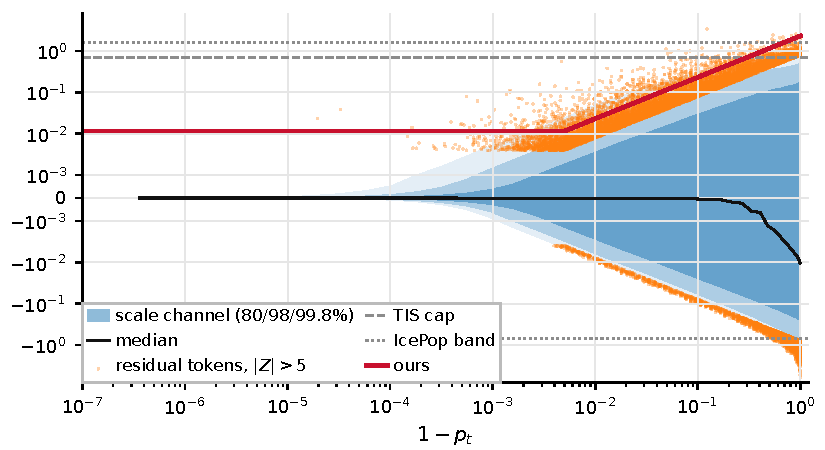
\includegraphics[width=\linewidth]{figures/mechanism.pdf}
\caption{Conditional distribution of $\log k_t$ against training-side uncertainty $1-p_t$ on the MoE model (12.3M tokens; symmetric-log vertical axis). Blue bands are the central 80\%, 98\%, and 99.8\% of tokens per uncertainty bin and follow the scale family of \Cref{def:two_channel} over six decades; the black line is the conditional median. Orange points are residual tokens with $|Z_t|>5$; at high confidence they lie above the shrinking bulk and are almost all positive. Grey lines are the constant thresholds of TIS ($\log 2$, dashed) and IcePop ($\log 0.5$ and $\log 5$, dotted), which lie above the entire distribution except at the least confident tokens. The red curve is the deployed one-sided band of \Cref{alg:cis}; its floor $\lambda_+\kappa=0.0115$ meets the residual layer at high confidence.}
\label{fig:mechanism}
\end{figure}

\noindent\textbf{Scale channel.}
Throughout this appendix $\varphi_t:=\max(1-p_t,\kappa)$ denotes the floored uncertainty of \Cref{alg:cis}, and $Z_t:=\log k_t/(c\varphi_t)$ the standardized deviation. Figure~\ref{fig:mechanism} shows the conditional distribution of $\log k_t$. Its width follows the scale family of \Cref{def:two_channel} across six decades of uncertainty, with $c=0.155$ for the MoE model and $c=0.035$ for the dense model and a weighted $R^2$ of $0.998$ over twenty equal-mass bins. After standardization by $c\varphi_t$ the central quantiles of $Z_t$ collapse across bins: between $\varphi=5\times10^{-3}$ and $\varphi=1$ the median moves by $0.06$ and the two deciles by $0.35$ and $1.17$ (Figure~\ref{fig:pivot}a). The upper tail is generalized Pareto with $\xi_+=0.49$ above the 99th percentile for the MoE model and $\xi_+=0.07$ for the dense model, so the MoE tail is heavy and some truncation is necessary rather than optional.

\noindent\textbf{Residual channel.}
We call a token residual when $|Z_t|>\zeta$ with the preregistered $\zeta=5$. Residual tokens are sparse, with $\hat\epsilon=1.26\%$ ($2.16\%$ at $\zeta=4$ and $0.78\%$ at $\zeta=6$), and their indicator is uncorrelated with $\varphi_t$ (correlation $0.004$). They cluster only weakly within trajectories: the lag-one autocorrelation of the indicator is $0.041$ against a permutation null of $0.0002$, and the conditional lift decays from $4.2$ at lag one to $2.6$ at lag four. At high confidence ($\varphi<0.05$) the residual displacement is one-sided, with $97.7\%$ of residual tokens positive on the base model and $100\%$ on the trained policy, and it is bounded, with a 99th percentile of $0.33$. Residual tokens are enriched in hard routing flips, which we define as a route change with gate margin above $10^{-3}$, by a factor of $1.46$ over the base rate of $0.53$, and they carry $2.0$ flipped layers on average against $1.1$ overall; the enrichment is real but not decisive, so routing is one contributor to the residual channel rather than its only cause. On the base model the residual median magnitude still scales with $\varphi$, at a fixed factor of about six above the bulk (Figure~\ref{fig:dualscale}a). The non-scaling behavior of \Cref{def:two_channel} appears once the policy has been trained and once the two engines are displaced in version. On the same tokens scored under a snapshot that is 29 steps stale, and in the logs of the training run itself, the residual magnitude at $\varphi<0.02$ lies between $0.04$ and $0.11$ while $c\varphi$ lies one to two orders of magnitude below it (Figure~\ref{fig:dualscale}b,c). We therefore state the non-scaling envelope as a high-confidence property, which is the regime in which \Cref{thm:cis_informal} is invoked. The paired measurement also fixes the sign structure of version displacement: rescoring the same tokens under the same snapshot through the two decode paths gives exactly zero difference, the displacement between snapshots is two-sided overall ($48.9\%$ positive) with a negative median at low confidence which reflects policy sharpening, and it is entirely positive on the high-confidence residual tokens that the operator acts on.

\noindent\textbf{Null measurements on the $\epsilon=0$ section.}
When $\epsilon=0$ the robust risk~\eqref{eq:robust_risk} reduces to an average-case criterion, and such criteria do not produce a confidence-dependent band; the band is a consequence of $\epsilon>0$. Four independent measurements on the same logs agree with this prediction. The sequence-level surface $\Delta(\varphi)$ has slope $-0.002$ with a trajectory-bootstrap interval of $[-0.48,0.15]$ over $20{,}000$ trajectories; the coupling coefficient $\lambda_{\mathrm{eff}}=c(\beta_1-\tfrac32\beta_2)$ has an interval which covers zero in three independent batches; the bare leave-one-out sum has slope $0.31$ against $\varphi$, of which $0.25$ survives a permutation that destroys within-trajectory coupling; and best-response iteration of the sequence-level risk converges from every start to a constant cap with $\lambda^\star=0.07$. The cross-layer coherence check gives a far-layer gradient coherence of $0.10$ between confidence layers, which is indistinguishable from its permutation null, and within a layer the token gradient directions are nearly orthogonal ($\rho\approx0.005$). These measurements support the scale channel and the sparsity, sign, and boundedness of the residual channel, with the qualification that the non-scaling envelope is a high-confidence property.

\subsection{Training Dynamics}
\label{app:experimental-dynamics}

\begin{figure}[h]
\centering

\includegraphics[width=0.9\linewidth]{figures/dyn_legend.pdf}\\[2pt]
\begin{minipage}[t]{0.325\linewidth}\centering
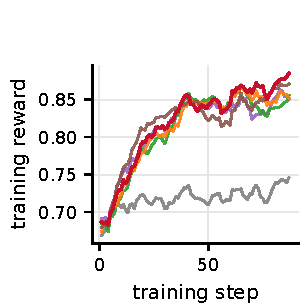
\includegraphics[width=\linewidth]{figures/dyn_reward.pdf}\\[-2pt]{\small (a)}
\end{minipage}\hfill
\begin{minipage}[t]{0.325\linewidth}\centering
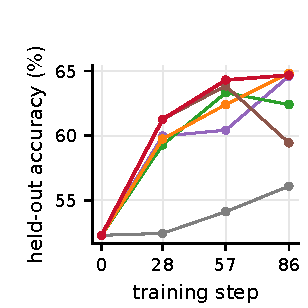
\includegraphics[width=\linewidth]{figures/dyn_heldout.pdf}\\[-2pt]{\small (b)}
\end{minipage}\hfill
\begin{minipage}[t]{0.325\linewidth}\centering
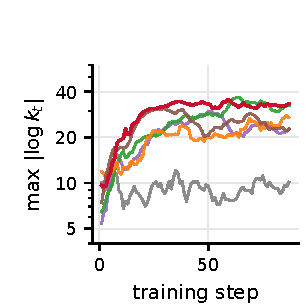
\includegraphics[width=\linewidth]{figures/dyn_gapmax.pdf}\\[-2pt]{\small (c)}
\end{minipage}\\[4pt]
\begin{minipage}[t]{0.325\linewidth}\centering
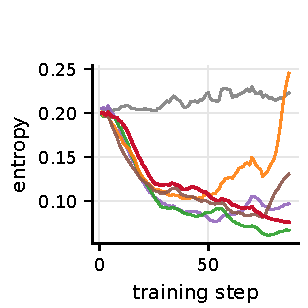
\includegraphics[width=\linewidth]{figures/dyn_entropy.pdf}\\[-2pt]{\small (d)}
\end{minipage}\hfill
\begin{minipage}[t]{0.325\linewidth}\centering
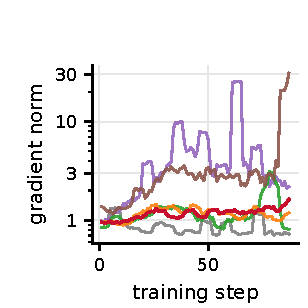
\includegraphics[width=\linewidth]{figures/dyn_grad.pdf}\\[-2pt]{\small (e)}
\end{minipage}\hfill
\begin{minipage}[t]{0.325\linewidth}\centering
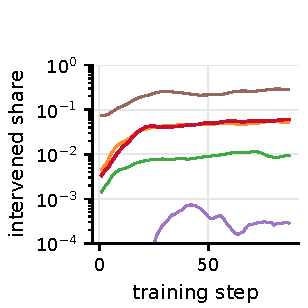
\includegraphics[width=\linewidth]{figures/dyn_rs.pdf}\\[-2pt]{\small (f)}
\end{minipage}
\caption{Training dynamics of the six operators under one recipe (seed one; curves smoothed over five steps). (a) Training reward. (b) Held-out accuracy of the epoch checkpoints, starting from the untrained model: the deployed operator leads at every checkpoint ($61.3$, $64.3$, $64.7$), and the KL mask peaks at $63.8$ after two epochs and falls to $59.4$ in the last one. (c) Largest $|\log k_t|$ in the batch, which grows during training for every corrected run as the policy sharpens. (d) Policy entropy. (e) Gradient norm: the exact ratio is spiky and the KL mask diverges late, whereas the cap, the gate, and the band stay near one. (f) Fraction of loss tokens intervened on by each operator; the KL mask removes about a fifth of all tokens.}
\label{fig:dynamics}
\end{figure}

Figure~\ref{fig:dynamics} shows the training dynamics of the six operators of Table~\ref{tab:main} under one recipe. The dynamics separate the methods more clearly than the endpoints. On the held-out epoch checkpoints (panel b) CIS is ahead at every epoch, with $61.3$, $64.3$, and $64.7$, and it is the only method whose accuracy does not dip in any epoch. The exact ratio has a healthy reward curve but a gradient norm which spikes to ten. The KL mask peaks at $63.8$ after two epochs and falls to $59.4$ in the last one, and its gradient norm diverges in the last epoch, whereas the cap, the gate, and the band stay near a gradient norm of one. The largest $|\log k_t|$ in the batch grows during training for every corrected run as the policy sharpens (panel c), which is the training-time growth of the scale constant discussed in Appendix~\ref{app:experimental-trigger}.

\subsection{Ablations of the Operator}
\label{app:experimental-ablation}

\begin{table}[h]
\centering
\caption{Single-variable ablations of the deployed operator (seed one unless stated). Each row changes one element of \Cref{alg:cis}; the slope sweep is in Table~\ref{tab:tuning}. Lifting the lower side and raising the floor leave the training reward unchanged or higher while lowering held-out accuracy; the row in bold reaches the highest training reward of the study and the held-out accuracy of no correction.}
\label{tab:ablation}
\small
\begin{tabular}{llcc}
\toprule
Element & Variant & Held-out (\%) & Train reward \\
\midrule
Deployed & $\lambda_-=\infty$, $\lambda_+=2.3$, $\kappa=5\times10^{-3}$ & 64.67 & 0.867 \\
Lower side & lift to $w\ge0.001$ & 63.15 & 0.851 \\
Lower side & \textbf{lift to $w\ge0.1$} & \textbf{56.10} & \textbf{0.878} \\
Lower side & symmetric band, $\lambda_-=1.0$ & 48.98 & 0.827 \\
Floor & none ($\kappa\to0$) & diverged at step 79 & --- \\
Floor & $\kappa=0.1$ (three seeds) & $61.01\pm0.83$ & 0.857--0.877 \\
Band shape & affine, $+0.12$ added to the band & 62.85 & 0.838 \\
\bottomrule
\end{tabular}
\end{table}

\noindent\textbf{One-sidedness and dose response.}
Table~\ref{tab:ablation} varies one element of the operator at a time. Lifting the lower side degrades held-out accuracy monotonically with the amount of lifting: from $64.67$ with no lower bound to $63.15$ at $w\ge0.001$, to $56.10$ at $w\ge0.1$, and to $48.98$ for the symmetric band, which is below the untrained model. The training reward does not register this harm; the $w\ge0.1$ variant reaches the highest training reward of the entire study while its held-out accuracy returns to the uncorrected level. An intermediate checkpoint of that run scores $62.62$ after one epoch and $56.10$ after three, so the harm accumulates as the policy sharpens and more tokens fall into the lifted region. Together with the support bound $k_t\ge p_t$, this is the empirical basis for restricting to the shrinkage class $\Mdown$ of \Cref{sec:prelim_estimation}.

\noindent\textbf{Floor and band shape.}
Without a floor the band collapses at high confidence: in the third epoch $32\%$ of tokens are truncated, the truncated tokens have median $|\log k_t|=7\times10^{-4}$, which is the resolution of the stored log-probabilities, and training diverges at step 79. With $\kappa=5\times10^{-3}$ the truncated tokens have median $|\log k_t|$ between $0.08$ and $0.12$. Raising the floor to $\kappa=0.1$, which places $58\%$ of tokens under a constant cap of $0.23$, costs $3.3$ points on three seeds while leaving the training reward unchanged; the floor is the storage resolution, not the residual scale. Adding a constant $0.12$ to the band costs $1.8$ points, which agrees with the null measurements of Appendix~\ref{app:experimental-twochannel}: the data support a multiplicative band and do not support additive widening. The slope sweep is reported in Section~\ref{sec:experiments-tuning}. In sum, the lower side must be left open, the floor must sit at the storage resolution, and the band must scale multiplicatively with $\varphi_t$.

\subsection{The Compilation Chain}
\label{app:experimental-compile}

\begin{table}[h]
\centering
\caption{The compilation chain of \Cref{thm:cis_informal}. Every input is measured without a training run; the output is compared with the slope that the RL sweep selects. The exceedance check compares $\Pr(Z>\lambda_+/c)$ at the deployed slope with the independently measured version-staleness rate. The FP8 row applies the proportionality rule to a changed serving configuration.}
\label{tab:compile}
\footnotesize\setlength{\tabcolsep}{3.5pt}
\begin{tabular}{lcccccc}
\toprule
Configuration & $c$ & $\xi_+$ & $\hat\epsilon$ & $\tau^\star$ & $\lambda_+=c\tau^\star$ & RL optimum / outcome \\
\midrule
bf16, base model & 0.155 & 0.49 & 0.0176 & 5.7 & 0.9 & 64.44 at 0.9; plateau $\{0.9,1.6,2.3\}$ \\
bf16, early training & 0.61 & --- & --- & 5.7 & 3.5 & deployed 2.3 in between \\
Exceedance check & \multicolumn{6}{l}{$\Pr(Z>\lambda_+/c)=0.13\%$ vs.\ staleness rate $0.5$--$0.6\%$ (same order)} \\
FP8 KV cache & 1.75 & --- & --- & --- & $2.3\times2.9=6.7$ & 63.00 vs.\ 60.12 at 2.3 \\
\bottomrule
\end{tabular}
\end{table}

\noindent\textbf{Compilation.}
Table~\ref{tab:compile} runs the compilation chain of \Cref{thm:cis_informal} on the measured constants. With $\hat\epsilon=1.76\%$ measured off the quantization floor and the empirical $F_Z$, the equalizer condition that fixes $\tau^\star$ in \Cref{thm:cis_informal}, $H(\tau)/\tau=\epsilon/(2-\epsilon)$ with $H(\tau)=\E[(Z-\tau)_+]$, has the root $\tau^\star=5.7$, which lies at the knee where the standardized bulk turns into the Pareto tail (Figure~\ref{fig:pivot}b,c). At the base-model scale this compiles to $\lambda_+=0.9$. The scale constant grows during training, from $0.16$ on the base model to $0.61$ in the first third of the run and $1.67$ in the last third, so the same $\tau^\star$ compiles to $3.5$ at the early-training scale. The deployed slope $\lambda_+=2.3$ lies between these two values. Running the compiled value itself gives $64.44$, which is on the same plateau as $1.6$ and $2.3$ ($64.67$ each), so the chain lands on the held-out optimum without any tuning, and the two compilations bracket the deployed slope in the direction in which $c$ moves during training. The exceedance check of the corollary also passes: at the deployed slope, $\Pr(Z>\lambda_+/c)=0.13\%$ against a version-staleness rate of $0.5$ to $0.6\%$ in the training logs, which is the same order of magnitude.

\subsection{Which Tokens the Band Acts On}
\label{app:experimental-trigger}

\begin{figure}[h]
\centering
\begin{minipage}[t]{0.325\linewidth}\centering
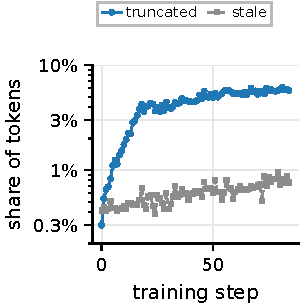
\includegraphics[width=\linewidth]{figures/trigger_a.pdf}\\[-2pt]{\small (a)}
\end{minipage}\hfill
\begin{minipage}[t]{0.325\linewidth}\centering
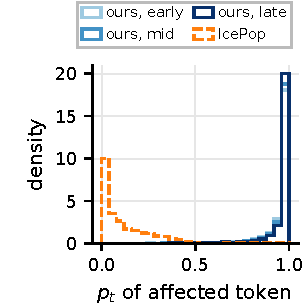
\includegraphics[width=\linewidth]{figures/trigger_b.pdf}\\[-2pt]{\small (b)}
\end{minipage}\hfill
\begin{minipage}[t]{0.325\linewidth}\centering
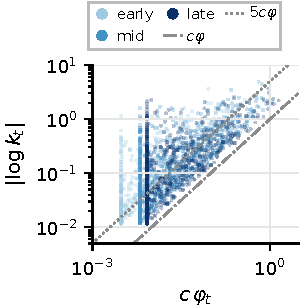
\includegraphics[width=\linewidth]{figures/trigger_c.pdf}\\[-2pt]{\small (c)}
\end{minipage}
\caption{What the band acts on during training (deployed operator, seed one; tokens logged every ten optimizer calls). (a) Fraction of truncated tokens per step (blue) and share of tokens whose rollout version is behind the current one (grey): the trigger rate rises from $0.3\%$ to about $5.5\%$ over the first forty steps and then stays flat, one order of magnitude above the stale share. (b) Training-side confidence $p_t$ of the affected tokens: the truncated tokens of our operator in the early, middle, and late third of training (blue, light to dark) concentrate at $p_t\to1$, whereas the tokens masked by IcePop in its own run (orange, dashed) concentrate at $p_t\to0$; the two operators act on complementary populations. (c) Magnitude $|\log k_t|$ of truncated tokens against the scale-channel width $c\varphi_t$ of their training phase, with $c$ fitted per phase; the dash-dotted and dotted lines mark $c\varphi_t$ and $5c\varphi_t$. Truncated tokens sit at $4$ to $7$ times the local width (median), and the vertical columns at the left are tokens on the floor $\varphi_t=\kappa$.}
\label{fig:trigger}
\end{figure}

Figure~\ref{fig:trigger} shows what the band does over the course of training. The trigger rate rises from $0.3\%$ to about $5.5\%$ during the first forty steps and then plateaus, one order of magnitude above the share of version-stale tokens, which stays between $0.4\%$ and $0.9\%$. Between $87\%$ and $90\%$ of the truncated tokens have $1-p_t<0.1$, and their median $|\log k_t|$ is $0.09$ to $0.10$ in every phase, which is $4$ to $7$ times the scale-channel width of that phase. In standardized training-time units, $49\%$ of the truncated tokens exceed $\zeta=5$ at $\lambda_+=2.3$ and $93\%$ do at $\lambda_+=6.7$, and among the truncated tokens the share of version-stale tokens is $3.0\%$, five times its base rate. Panel (b) is the clearest statement of the difference between the two operators: IcePop removes low-confidence tokens whose ratio leaves a fixed interval, and the band truncates high-confidence tokens whose displacement is large relative to their local width; the acceptance regions of all four operators are drawn in Figure~\ref{fig:regions} of the appendix. Panels (a) and (c) also record a fact about the training run itself: the scale constant grows from $0.61$ to $1.67$ between the first and last third of training while the width at high confidence stays small, so a slope calibrated on the base model becomes tighter in standardized units as training proceeds. This is the mechanism behind the FP8 result and the reason that the compilation $\lambda_+=c\tau^\star$ should be applied to the serving configuration at hand.

\subsection{Additional Tables and Figures}
\label{app:experimental-results}

\begin{table}[h]
\centering
\caption{Per-seed held-out GSM8K accuracy (\%, legacy last-number exact match) and training statistics behind Table~\ref{tab:main}. Reward is the mean training reward over the third epoch (mean$\pm$std over seeds); Intervened is the fraction of loss tokens that the operator truncated or masked (seed one); s/step is seconds per optimizer step on one node of eight A100 GPUs. No operator adds a forward or backward pass.}
\label{tab:main_seeds}
\footnotesize\setlength{\tabcolsep}{3pt}
\begin{tabular}{lccccccc}
\toprule
Method & Seed 1 & Seed 2 & Seed 3 & Mean$_{\pm\mathrm{std}}$ & Reward & Intervened (\%) & s/step \\
\midrule
No correction ($M\equiv1$) & 56.10 & 54.44 & 56.10 & $55.55_{\pm0.96}$ & $0.732_{\pm0.004}$ & 0 & 33 \\
Exact ratio ($M=k$) & 64.59 & 55.50 & 59.06 & $59.72_{\pm4.58}$ & $0.829_{\pm0.012}$ & 0 & 32 \\
KPop (binary-KL mask, $2$) & 59.44 & 59.29 & 57.85 & $58.86_{\pm0.88}$ & $0.848_{\pm0.010}$ & 21.9 & 31 \\
KPop$^\dagger$ (corrected) & 58.45 & 62.40 & 62.24 & $61.03_{\pm2.24}$ & $0.846_{\pm0.016}$ & 0.5 & 31 \\
IcePop (mask $[0.5,5]$) & \textbf{64.82} & 62.70 & 63.46 & $63.66_{\pm1.07}$ & $0.859_{\pm0.004}$ & 4.1 & 33 \\
TIS (cap $2$) & 62.40 & 63.91 & \textbf{65.43} & $63.91_{\pm1.52}$ & $0.861_{\pm0.014}$ & 0.8 & 32 \\
CIS (ours, \Cref{alg:cis}) & 64.67 & \textbf{64.97} & 63.23 & $\mathbf{64.29_{\pm0.93}}$ & $\mathbf{0.867_{\pm0.009}}$ & 4.2 & 34 \\
\bottomrule
\end{tabular}
\end{table}

\begin{table}[h]
\centering
\caption{Per-seed results for the as-shipped KPop mask and the baselines from outside the token-level operator class (five-benchmark protocol of Table~\ref{tab:main}): GSM8K accuracy and macro average over the five benchmarks per seed, mean training reward over the third epoch, and the fraction of responses on which the operator acts (Seq-TIS: capped; Seq-MIS: rejected). GSPO's reward peaks near $0.80$ in the second epoch on every seed and then collapses; FP16 has no operator.}
\label{tab:extra_seeds}
\footnotesize\setlength{\tabcolsep}{4pt}
\begin{tabular}{lcccccc}
\toprule
 & \multicolumn{3}{c}{GSM8K (seed 1 / 2 / 3)} & \multicolumn{3}{c}{Avg (seed 1 / 2 / 3)} \\
Method & & & & & & \\
\midrule
KPop (as shipped, binary-KL mask $2$) & 63.00 & 2.05 & 57.32 & 31.10 & 2.43 & 29.73 \\
Seq-TIS (cap $2$, product ratio) & 65.96 & 65.73 & 66.11 & 32.39 & 31.36 & 33.08 \\
Seq-MIS (mask $[0.5,2]$, product ratio) & 60.27 & 62.70 & 59.97 & 30.47 & 31.81 & 31.18 \\
GSPO (clip $3\times10^{-4}/4\times10^{-4}$) & 52.54 & 0.00 & 40.11 & 27.44 & 0.50 & 22.61 \\
FP16 (no operator) & 60.27 & 58.76 & 61.03 & 30.68 & 30.93 & 31.44 \\
\midrule
 & \multicolumn{3}{c}{Reward, epoch 3 (seed 1 / 2 / 3)} & \multicolumn{3}{c}{Responses acted on (\%)} \\
\midrule
Seq-TIS & 0.799 & 0.802 & 0.807 & 16.8 & 12.0 & 11.9 \\
Seq-MIS & 0.759 & 0.758 & 0.762 & 94.0 & 95.1 & 94.6 \\
GSPO & 0.340 & 0.032 & 0.541 & --- & --- & --- \\
FP16 & 0.741 & 0.738 & 0.739 & 0 & 0 & 0 \\
\bottomrule
\end{tabular}
\end{table}

\begin{figure}[h]
\centering
\begin{minipage}[t]{0.325\linewidth}\centering
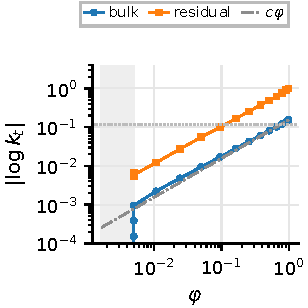
\includegraphics[width=\linewidth]{figures/dualscale_a.pdf}\\[-2pt]{\small (a)}
\end{minipage}\hfill
\begin{minipage}[t]{0.325\linewidth}\centering
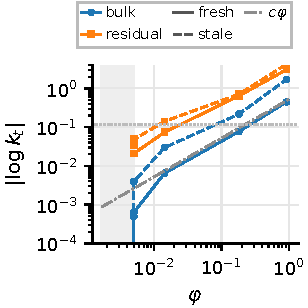
\includegraphics[width=\linewidth]{figures/dualscale_b.pdf}\\[-2pt]{\small (b)}
\end{minipage}\hfill
\begin{minipage}[t]{0.325\linewidth}\centering
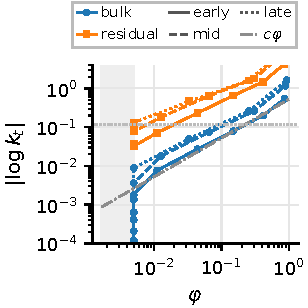
\includegraphics[width=\linewidth]{figures/dualscale_c.pdf}\\[-2pt]{\small (c)}
\end{minipage}
\caption{Bulk width and residual magnitude of $\log k_t$ against $\varphi$ in three regimes. Blue circles: median absolute deviation of $\log k_t$ per equal-mass bin (bulk). Orange squares: median $|\log k_t|$ of residual tokens ($|Z_t|>5$). Dashed line: $c\varphi$ with the fresh-engine constant of that panel; dotted line: $0.12$; shaded band: the quantization floor $\varphi<\kappa$; lighter to darker shades in (b) and (c) mark fresh versus stale and early versus late. (a) Base model with both engines at the same parameters: both curves scale with $\varphi$ and no additive layer is present. (b) The same trained-policy tokens scored with a fresh engine and with an engine 29 steps stale. (c) Tokens logged during the deployed-operator run, per training third, with the scale constant of that third. In (b) and (c) the residual magnitude at $\varphi<0.02$ lies between $0.04$ and $0.11$, one to two orders of magnitude above $c\varphi$, while at low confidence it remains a fixed multiple of the bulk.}
\label{fig:dualscale}
\end{figure}

\begin{figure}[h]
\centering
\begin{minipage}[t]{0.325\linewidth}\centering
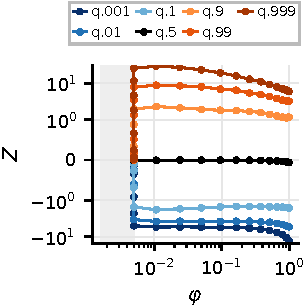
\includegraphics[width=\linewidth]{figures/pivot_a.pdf}\\[-2pt]{\small (a)}
\end{minipage}\hfill
\begin{minipage}[t]{0.325\linewidth}\centering
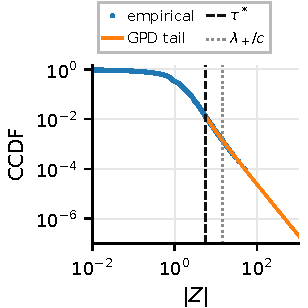
\includegraphics[width=\linewidth]{figures/pivot_b.pdf}\\[-2pt]{\small (b)}
\end{minipage}\hfill
\begin{minipage}[t]{0.325\linewidth}\centering
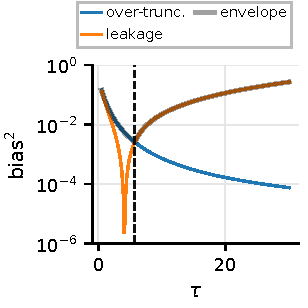
\includegraphics[width=\linewidth]{figures/pivot_c.pdf}\\[-2pt]{\small (c)}
\end{minipage}
\caption{Standardized view on the MoE model. (a) Quantiles $0.001$ to $0.999$ of $Z_t=\log k_t/(c\varphi_t)$ per equal-mass bin (blue to orange from lower to upper, black is the median): the central quantiles collapse across two decades of $\varphi$, the extreme quantiles drift and are asymmetric. (b) Complementary distribution of $|Z_t|$ off the floor (blue) with the generalized-Pareto fit above the 99th percentile (orange, $\xi_+=0.49$); the dashed line is the equalizer root $\tau^\star=5.7$, which sits at the transition from bulk to tail, and the dotted line is the deployed slope in the same units, $\lambda_+/c=14.8$. (c) The two branches of the worst-case bias of \Cref{thm:cis_informal} evaluated with the empirical $F_Z$ and $\hat\epsilon=0.0176$: the over-truncation branch $H(\tau)^2$ (blue) decreases in $\tau$, the leakage branch $[\epsilon\tau-(1-\epsilon)H(\tau)]^2$ (orange) increases, and their envelope (grey) is minimized at $\tau^\star$ (dashed).}
\label{fig:pivot}
\end{figure}


\begin{figure}[h]
\centering
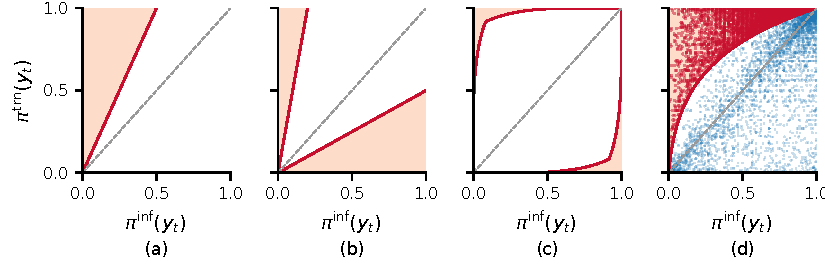
\includegraphics[width=\linewidth]{figures/regions.pdf}
\caption{Intervention regions of the four operators in the plane of the two engine probabilities of the sampled token, $\pi^{\mathrm{inf}}(y_t)$ (horizontal) and $\pi^{\mathrm{trn}}(y_t)$ (vertical); the shaded region is truncated or masked, the dashed line is $\pi^{\mathrm{trn}}=\pi^{\mathrm{inf}}$. (a) TIS caps the ratio at $2$. (b) IcePop masks outside $[0.5,5]$. (c) The Bernoulli-KL mask with threshold $2$ excludes only extreme corners of the plane by definition; the additional tokens it removes in practice are those with a probability of exactly one on either engine, which the metric maps to an undefined value (Section~\ref{sec:experiments-results}). (d) The deployed band truncates above a curve which approaches the diagonal as $\pi^{\mathrm{trn}}\to1$; blue points are a sample of kept tokens and red points the truncated tokens from the deployed-operator run, which sit at the top edge of the plane.}
\label{fig:regions}
\end{figure}

\begin{table}[h]
\centering
\caption{Intervention rate and cost per method (seed one). The intervened fraction is reported by the training framework as the fraction of loss tokens that were truncated or masked, averaged over the run; wall-clock time is the median time between consecutive optimizer steps on the same node type. Every operator is an elementwise map of two log-probability tensors that are already computed for the decoupled loss, so no method adds a forward or backward pass.}
\label{tab:overhead}
\small\setlength{\tabcolsep}{4pt}
\begin{tabular}{lcccc}
\toprule
Method & Intervened tokens (\%) & Seconds per step & Extra passes & Held-out (\%) \\
\midrule
No correction & 0 & 33 & none & 56.10 \\
Exact ratio & 0 & 32 & none & 64.59 \\
TIS & 0.8 & 32 & none & 62.40 \\
IcePop & 4.1 & 33 & none & 64.82 \\
KPop (as implemented) & 21.9 & 31 & none & 59.44 \\
KPop (numerically corrected) & 0.5 & 31 & none & 58.45 \\
Ours & 4.2 & 34 & none & 64.67 \\
\bottomrule
\end{tabular}
\end{table}

\noindent\textbf{The KL mask and probability saturation.}
The binary-KL metric of the KPop baseline is $\mathrm{KL}(\mathrm{Bern}(p)\,\|\,\mathrm{Bern}(q))=p\log(p/q)+(1-p)\log((1-p)/(1-q))$ evaluated in both directions, with $p$ and $q$ clamped to $[10^{-8},1-10^{-8}]$. In single precision the upper clamp is the identity, so a token whose probability is exactly one on both engines yields $0\cdot\log(0/0)$, and a token whose probability is exactly one on one engine yields $+\infty$; the bounds check treats both as out of bounds. On the tokens logged in the KPop run, $16.5\%$ have probability exactly one on both engines and $2.8\%$ on one engine, which together with the $0.45\%$ of tokens whose finite metric exceeds the threshold reproduces the $22\%$ intervention rate that the framework reports. Recomputing the metric in double precision with a representable clamp and mapping the undefined case to zero gives a mask rate of $0.45\%$. We report the framework's implementation as run in the main text because it is the implementation practitioners obtain. A numerically corrected variant, run under the same recipe with three seeds, scores $58.45$, $62.40$, and $62.24$ ($61.03\pm2.24$), which lifts the KL mask by about two points but leaves it below the cap, the gate, and the band; the residual gap is consistent with the mask acting on a fixed KL threshold that does not follow the confidence-dependent width of the mismatch.

\begin{table}[h]
\centering
\caption{Trigger statistics of the band on the tokens logged during the deployed-operator run, for several slopes applied to the same tokens. Residual precision is the share of truncated tokens with $|Z_t|>5$ in training-time units; stale precision is the share with rollout version behind the current one; enrichment is stale precision divided by the base staleness rate of $0.58\%$.}
\label{tab:trigger}
\small
\begin{tabular}{cccccc}
\toprule
$\lambda_+$ & Truncated (\%) & Share at $1-p_t<0.1$ & Residual precision & Stale precision & Enrichment \\
\midrule
1.0 & 7.14 & 0.82 & 0.26 & 0.022 & 3.8 \\
1.6 & 5.16 & 0.86 & 0.37 & 0.026 & 4.5 \\
2.3 & 3.89 & 0.89 & 0.49 & 0.030 & 5.1 \\
3.1 & 3.05 & 0.91 & 0.62 & 0.033 & 5.8 \\
4.0 & 2.45 & 0.93 & 0.70 & 0.037 & 6.5 \\
6.7 & 1.57 & 0.96 & 0.93 & 0.045 & 7.8 \\
\bottomrule
\end{tabular}
\end{table}

\begin{table}[h]
\centering
\caption{Dose--response of lower-side lifting (seed one). The training reward is the mean over the third epoch; the held-out accuracy of the intermediate checkpoint after one epoch is given where it was evaluated.}
\label{tab:dose}
\small
\begin{tabular}{lcccc}
\toprule
Lower side & Held-out (\%) & Held-out after epoch 1 & Train reward & Peak reward \\
\midrule
none ($\lambda_-=\infty$) & 64.67 & --- & 0.867 & 0.897 \\
lift to $w\ge0.001$ & 63.15 & --- & 0.851 & 0.898 \\
lift to $w\ge0.1$ & 56.10 & 62.62 & 0.878 & 0.910 \\
symmetric band, $\lambda_-=1.0$ & 48.98 & --- & 0.827 & 0.869 \\
\bottomrule
\end{tabular}
\end{table}

\section{Additional Results and Scope}
\label{app:discussion}

\paragraph{Uniform bias rather than finite-sample MSE.}
\Cref{thm:band-capping,thm:localized-gating,prop:posterior-gate} optimize a uniform bias constant or its integrated analogue. Sampling variance is not part of the population criterion except for the calibration bound in \Cref{thm:band-capping}. Adding finite-sample MSE generally creates an interior bias--variance tradeoff and requires second moments, sample size, and a covariance model.

\paragraph{Localization is a theorem condition.}
The statistical separation between capping and zeroing comes from restricting the corrupted ratio support to $\Lset$. Payload-validity diagnostics must test whether corrupted tokens are concentrated in the declared region. If localization fails, \Cref{eq:nonidentifiability-gap} is the safe comparison and zeroing has no class-wide advantage over the cap at the same upper level.

\paragraph{The escape set is estimated in practice.}
\Cref{thm:localized-gating} conditions on a fixed $\Lset$. Replacing it by $\widehat\Lset$ adds clean fidelity error bounded by
\begin{equation}
B\E_{P_0}[K\1\{K\in\Lset\triangle\widehat\Lset\}],
\end{equation}
while the true reachable-set supremum may change discontinuously unless physical reachability near the estimated boundary is controlled. The calibration rule should therefore be frozen and its boundary sensitivity reported separately.

\paragraph{True supremum versus essential supremum.}
The localized class permits a corrupted law to concentrate on a physically reachable ratio that has zero clean probability. This is why \Cref{eq:localized-risk} uses a true supremum over $\Lset$, not a $P_0$-essential supremum. The fixed-density model in \Cref{eq:density-risk} instead integrates with respect to $g$ and is insensitive to $g$-null points.

\paragraph{Channel separability.}
The matching constructions in \Cref{lem:joint-risk} independently choose clean and corrupted conditional payload means and align them along a common vector. This is appropriate for the latent-channel class in \Cref{eq:localized-class}. If a physical constraint forces both channels to share the same payload map at every overlapping ratio, \Cref{eq:localized-risk} remains an upper bound, but exact equality may fail.

\paragraph{Unknown side allocation.}
\Cref{cor:two-sided} assumes fixed masses $\eps_-$ and $\eps_+$. If only total mass $\eps$ is fixed and its side allocation is unspecified, the exposure term becomes
\begin{equation}
\eps B\max\left\{\sup_{k\in\Lset_-}\abs{M(k)},\sup_{k\in\Lset_+}\abs{M(k)}\right\}.
\end{equation}
The side problems no longer separate. The fixed-mass formulation should therefore be used only when side-specific route-disagreement rates are stable enough to support it.
\end{document}

